% Arquivo LaTeX de exemplo de dissertação/tese a ser apresentada à CPG do IME-USP
%
% Criação: Jesús P. Mena-Chalco
% Revisão: Fabio Kon e Paulo Feofiloff
% Adaptação para UTF8, biblatex e outras melhorias: Nelson Lago
%
% Except where otherwise indicated, these files are distributed under
% the MIT Licence. The example text, which includes the tutorial and
% examples as well as the explanatory comments in the source, are
% available under the Creative Commons Attribution International
% Licence, v4.0 (CC-BY 4.0) - https://creativecommons.org/licenses/by/4.0/


%%%%%%%%%%%%%%%%%%%%%%%%%%%%%%%%%%%%%%%%%%%%%%%%%%%%%%%%%%%%%%%%%%%%%%%%%%%%%%%%
%%%%%%%%%%%%%%%%%%%%%%%%%%%%%%% PREÂMBULO LaTeX %%%%%%%%%%%%%%%%%%%%%%%%%%%%%%%%
%%%%%%%%%%%%%%%%%%%%%%%%%%%%%%%%%%%%%%%%%%%%%%%%%%%%%%%%%%%%%%%%%%%%%%%%%%%%%%%%
\documentclass[12pt,twoside,brazil,english]{book}
\usepackage[a4paper]{geometry}

\geometry{
  %top=32mm,
  %bottom=28mm,
  %left=24mm,
  %right=34mm,
  textwidth=152mm, % 210-24-34
  textheight=237mm, % 297-32-28
  vmarginratio=8:7, % 32:28
  hmarginratio=12:17, % 24:34
  % Com geometry, esta medida não é tão relevante; basta garantir que ela
  % seja menor que "top" e que o texto do cabeçalho caiba nela.
  headheight=25.4mm,
  % distância entre o início do texto principal e a base do cabeçalho;
  % ou seja, o cabeçalho "invade" a margem superior nessa medida. Essa
  % é a medida que determina a posição do cabeçalho
  headsep=11mm,
  footskip=10mm,
  marginpar=20mm,
  marginparsep=5mm,
}

% Vários pacotes e opções de configuração genéricos; para personalizar o
% resultado, modifique estes arquivos.
%%%%%%%%%%%%%%%%%%%%%%%%%%%%%%%%%%%%%%%%%%%%%%%%%%%%%%%%%%%%%%%%%%%%%%%%%%%%%%%%
%%%%%%%%%%%%%%%%%%%%%%% CONFIGURAÇÕES E PACOTES BÁSICOS %%%%%%%%%%%%%%%%%%%%%%%%
%%%%%%%%%%%%%%%%%%%%%%%%%%%%%%%%%%%%%%%%%%%%%%%%%%%%%%%%%%%%%%%%%%%%%%%%%%%%%%%%

% Vários comandos auxiliares para o desenvolvimento de packages e classes;
% aqui, usamos em alguns comandos de formatação e condicionais.
\usepackage{etoolbox}
\usepackage{xstring}
\usepackage{xparse}
\usepackage{regexpatch}
% Algumas packages dependem de xpatch e tentam carregá-la, causando conflitos
% com regexpatch. Como regexpatch oferece todos os recursos de xpatch (ela
% é uma versão estendida de xpatch, mas ainda considerada experimental), vamos
% fazê-las acreditar que xpatch já foi carregada.
\expandafter\xdef\csname ver@xpatch.sty\endcsname{2012/10/02}

\usepackage{calc}
% Sempre que possível, é melhor usar os recursos de etoolbox ao invés de
% ifthen; no entanto, várias packages dependem dela.
%\usepackage{ifthen}
% Estas não estão em uso mas podem ser úteis.
%\usepackage{ltxcmds}
%\usepackage{letltxmacro}

% Esta package permite detectar XeTeX, LuaTeX e pdfTeX, mas pode não estar
% disponível em todas as instalações de TeX.
%\usepackage{iftex}
% Por conta disso, usaremos estas (que não detectam pdfTeX):
\usepackage{ifxetex}
\usepackage{ifluatex}

\newbool{unicodeengine}
\ifboolexpr{bool{xetex} or bool{luatex}}
  {\booltrue{unicodeengine}}
  {\boolfalse{unicodeengine}}

% Detecta se estamos produzindo um arquivo PDF ou DVI (lembrando que tanto
% pdfTeX quanto LuaTeX podem gerar ambos)
\usepackage{ifpdf}

% Algumas packages "padrão" da AMS, que são praticamente  obrigatórias.
% Algumas delas devem ser carregadas antes de unicode-math ou das
% definições das fontes do documento.
\usepackage{amssymb}
\usepackage{amsthm}
\usepackage{amsmath}
\usepackage{mathtools}

% "fontenc" é um parâmetro do NFSS (sistema de gestão de fontes do
% LaTeX; consulte "texdoc fntguide" e "texdoc fontenc"). O default
% é OT1, mas ele tem algumas limitações; a mais importante é que,
% com ele, palavras acentuadas não podem ser hifenizadas. Por
% conta disso, quase todos os documentos LaTeX utilizam o fontenc
% T1. A escolha do fontenc tem consequências para as fontes que
% podem ser usadas com NFSS; hoje em dia T1 tem mais opções de
% qualidade, então não se perde nada em usá-lo. A package fontspec
% (para gestão de fontes usando outro mecanismo, compatível apenas
% com lualatex e xelatex) carrega fontenc automaticamente, mas
% usando outra codificação ("TU" e não "T1"). Ainda assim, é útil
% carregar o fontenc T1 (antes de carregar fontspec!) para o caso
% de alguma fonte "antiga" ser utilizada no documento (embora isso
% não seja recomendado: lualatex e xelatex só são capazes de
% hifenizar palavras acentuadas com o fontenc TU).
\usepackage[T1]{fontenc}

\ifunicodeengine
  % Não é preciso carregar inputenc com LuaTeX e XeTeX, pois
  % com eles utf8 é obrigatório.
  \usepackage{fontspec}

  % Ao invés de usar o sistema tradicional de LaTeX para gerir
  % as fontes matemáticas, utiliza as extensões matemáticas do
  % formato otf definidas pela microsoft. Ao ativar esta package
  % o mecanismo tradicional não funciona mais! Há poucas fontes
  % com suporte a unicode-math.
  \usepackage{unicode-math}
\else
  % O texto está escrito em utf8.
  \usepackage[utf8]{inputenc}

  % Permitem utilizar small caps + itálico (e outras pequenas
  % melhorias). Em geral, desnecessário com fontenc, a menos
  % que alguma package utilize especificamente. Algumas raras
  % packages de fontes podem causar conflitos com fontaxes, em
  % geral por utilizarem a package "concorrente" nfssext-cfr.
  \usepackage{fontaxes}
  \usepackage{mweights}
\fi

% Acesso a símbolos adicionais, como \textrightarrow, \texteuro etc.,
% disponíveis na maioria das fontes através do fontenc TS1 ou mudando
% momentaneamente para computer modern/latin modern. Raramente útil
% com lualatex/xelatex, mas não causa problemas. Várias packages de
% fontes carregam textcomp, às vezes com opções específicas; assim,
% para evitar problemas, vamos carregá-la no final do preâmbulo para
% o caso de ela não ter sido carregada antes.
\AtBeginDocument{\usepackage{textcomp}}

% Internacionalização dos nomes das seções ("chapter" X "capítulo" etc.),
% hifenização e outras convenções tipográficas. babel deve ser um dos
% primeiros pacotes carregados. É possível passar a língua do documento
% como parâmetro aqui, mas já fizemos isso ao carregar a classe, no início
% do documento.
\usepackage{babel}

% É possível personalizar as palavras-chave que babel utiliza, por exemplo:
%\addto\extrasbrazil{\renewcommand{\chaptername}{Chap.}}
% Com BibTeX, isso vale também para a bibliografia; com BibLaTeX, é melhor
% usar o comando "DefineBibliographyStrings".

% Para línguas baseadas no alfabeto latino, como o inglês e o português,
% o pacote babel funciona muito bem, mas com outros alfabetos ele às vezes
% falha. Por conta disso, o pacote polyglossia foi criado para substituí-lo.
% polyglossia só funciona com LuaTeX e XeTeX; como babel também funciona com
% esses sistemas, provavelmente não há razão para usar polyglossia, mas é
% possível que no futuro esse pacote se torne o padrão.
%\usepackage{polyglossia}
%\setdefaultlanguage{brazil}
%\setotherlanguage{english}

% Alguns pacotes (espeficicamente, tikz) usam, além de babel, este pacote
% como auxiliar para a tradução de palavras-chave, como os meses do ano.
\usepackage{translator}

% microajustes no tamanho das letras, espaçamento etc. para melhorar
% a qualidade visual do resultado. LaTeX tradicional não dá suporte a
% nenhum tipo de microajuste; pdfLaTeX dá suporte a todos. LuaLaTeX
% e XeLaTeX dão suporte a alguns:
%
% * expansion não funciona com XeLaTeX
% * tracking não funciona com XeLaTeX; é possível obter o mesmo resultado
%   com a opção "LetterSpace" do pacote fontspec, mas a configuração é
%   totalmente manual. Por padrão, aumenta o afastamento entre caracteres
%   nas fontes "small caps"; o resultado não se presta ao uso na
%   bibliografia ou citações, então melhor desabilitar.
% * kerning e spacing só funcionam com pdfLaTex; ambas são funções
%   consideradas experimentais e nem sempre produzem resultados vantajosos.

\newcommand\microtypeopts{
  protrusion=true,
  tracking=false,
  kerning=false,
  spacing=false
}

% TeXLive 2018 inclui a versão 2.7a da package microtype e a versão
% 1.07 de luatex. Essa combinação faz aparecer um bug:
% https://tex.stackexchange.com/questions/476740/microtype-error-with-lualatex-attempt-to-call-field-warning-a-nil-value
% Aqui, aplicamos a solução sugerida, que não tem "contra-indicações".
\ifluatex
  \usepackage{luatexbase}
\fi

\ifxetex
  \usepackage[expansion=false,\microtypeopts]{microtype}
\else
  \usepackage[expansion=true,\microtypeopts]{microtype}
\fi

% Alguns "truques" (sujos?) para minimizar over/underfull boxes.
%
% Para fazer um texto justificado, é preciso modificar o tamanho dos espaços
% em cada linha para mais ou para menos em relação ao seu tamanho ideal. Para
% escolher as quebras de linha, TeX vai percorrendo o texto procurando lugares
% possíveis para quebrar as linhas considerando essa flexibilidade mas dentro
% de um certo limite mínimo/máximo. Nesse processo, ele associa a cada possível
% linha o valor *badness*, que é o nível de distorção do tamanho dos espaços
% daquela linha em relação ao ideal, e ignora opções que tenham badness muito
% grande (esse limite é dado por \tolerance). Depois de encontradas todas
% as possíveis quebras de linha e a badness de cada uma, TeX calcula as
% *penalties* das quebras encontradas, que são uma medida de quebras "ruins".
% Por exemplo, na configuração padrão, quebrar uma linha hifenizando uma
% palavra gera uma penalty de 50; já uma quebra que faça a última linha
% do parágrafo ficar sozinha na página seguinte gera uma penalty de 150.
% Finalmente, TeX calcula a "feiúra" de cada possível linha (demerits)
% com base na badness e nas penalties e escolhe a solução que minimiza os
% demerits totais do parágrafo. Os comandos \linebreak e \pagebreak funcionam
% simplesmente acrescentando uma penalty negativa ao lugar desejado para a
% quebra.
%
% Para cada fonte, o espaço em TeX tem um tamanho ideal, um tamanho mínimo e um
% tamanho máximo. TeX nunca reduz um espaço para menos que o mínimo da fonte,
% mas pode aumentá-lo para mais que o máximo. Se os espaços de uma linha ficam
% com o tamanho ideal, a badness da linha é 0; se o tamanho é
% reduzido/aumentado 50% do mínimo/máximo, a badness da linha é 12; se o
% tamanho é reduzido/aumentado para o mínimo/máximo, a badness é 100. Se esse
% aumento for de 30% além do máximo, a badness da linha é 200; se for de 45%
% além do máximo, a badness é 300; se for de 60% além do máximo, a badness é
% 400; se for de 100% além do máximo, a badness é 800. O valor máximo possível
% para badness é 10.000, que significa "badness infinita".
%
% \tolerance indica a badness máxima que TeX aceita para uma linha; seu valor
% default é 200. Assim, aumentar para, digamos, 300 ou 400, permite que
% TeX escolha parágrafos com maior variação no espaçamento entre as linhas.
% No entanto, no cálculo de demerits, a badness e as penalties de cada linha
% são elevadas ao quadrado, então TeX geralmente prefere escolher outras
% opções no lugar de uma linha ruim. Por exemplo, órfãs/viúvas têm demerit
% de 22.500 e dois hífens seguidos têm demerit de 10.000; já uma linha com
% badness 400 tem demerit 160.000. Portanto, não é surpreendente que a maioria
% dos parágrafos tenha demerits abaixo de 40.000, quase todos abaixo de 100.000
% e praticamente nenhum acima de 1.000.000. Isso significa que, para a grande
% maioria dos parágrafos, aumentar \tolerance não faz diferença: uma linha com
% badness 400 nunca será efetivamente escolhida se houver qualquer outra opção
% com badness menor. Também fica claro que não há muita diferença real entre
% definir \tolerance como 800 ou 9.999.
%
% O problema muda de figura se TeX não consegue encontrar uma solução. Isso
% pode acontecer em dois casos: (1) o parágrafo tem ao menos uma linha que não
% pode ser quebrada com badness < 10.000 ou (2) o parágrafo tem ao menos uma
% linha que não pode ser quebrada com badness < tolerance (mas essa badness é
% menor que 10.000).
%
% No primeiro caso, se houver várias possibilidades de linhas que não podem ser
% quebradas, TeX não vai ser capaz de compará-las e escolher a melhor: todas
% têm a badness máxima (10.000) e, portanto, a que gerar menos deméritos no
% restante do parágrafo será a escolhida. Na realidade, no entanto, essas
% linhas *não* são igualmente ruins entre si, o que pode levar TeX a fazer uma
% má escolha. Para evitar isso, TeX tenta novamente aplicando
% \emergencystretch, que "faz de conta" que o tamanho máximo ideal dos espaços
% da linha é maior que o definido na fonte. Isso reduz a badness de todas as
% linhas, o que soa parecido com aumentar \tolerance. Há três diferenças, no
% entanto: (1) essa mudança só afeta os parágrafos que falharam; (2) soluções
% que originalmente teriam badness = 10.000 (e, portanto, seriam vistas como
% equivalentes) podem ser avaliadas e comparadas entre si; e (3) como a badness
% de todas as linhas diminui, a possibilidade de outras linhas que
% originalmente tinham badness alta serem escolhidas aumenta. Esse último ponto
% significa que \emergencystretch pode fazer TeX escolher linhas mais
% espaçadas, fazendo o espaçamento do parágrafo inteiro aumentar e, portanto,
% tornando o resultado mais homogêneo mesmo com uma linha particularmente ruim.
%
% É esse último ponto que justifica o uso de \emergencystretch no segundo caso
% também: apenas aumentar a tolerância, nesse caso, poderia levar TeX a
% diagramar uma linha ruim em meio a um parágrafo bom, enquanto
% \emergencystretch pode fazer TeX aumentar o espaçamento de maneira geral no
% parágrafo, minimizando o contraste da linha problemática com as demais.
% Colocando a questão de outra maneira, aumentar \tolerance para lidar com
% esses parágrafos problemáticos pode fazê-los ter uma linha especialmente
% ruim, enquanto \emergencystretch pode dividir o erro entre várias linhas.
% Assim, definir \tolerance em torno de 800 parece razoável: no caso geral,
% não há diferença e, se um desses casos difíceis não pode ser resolvido com
% uma linha de badness até 800, \emergencystretch deve ser capaz de gerar um
% resultado igual ou melhor.
%
% Penalties & demerits: https://tex.stackexchange.com/a/51264
% Definições (fussy, sloppy etc.): https://tex.stackexchange.com/a/241355
% Mais definições (hfuzz, hbadness etc.): https://tex.stackexchange.com/a/50850
% Donald Arseneau defendendo o uso de \sloppy: https://groups.google.com/d/msg/comp.text.tex/Dhf0xxuQ66E/QTZ7aLYrdQUJ
% Artigo detalhado sobre \emergencystretch: https://www.tug.org/TUGboat/tb38-1/tb118wermuth.pdf
% Esse artigo me leva a crer que algo em torno de 1.5em é suficiente

\tolerance=800
\hyphenpenalty=100 % Default 50; se o texto é em 2 colunas, 50 é melhor
\setlength{\emergencystretch}{1.5em}

% Não gera warnings para Overfull menor que 0.5pt
\hfuzz=.5pt
\vfuzz\hfuzz

% Não gera warnings para Underfull com badness < 1000
\hbadness=1000
\vbadness=1000

% Por padrão, o algoritmo LaTeX para textos não-justificados é (muito) ruim;
% este pacote implementa um algoritmo bem melhor
\usepackage[newcommands]{ragged2e}

% ragged2e funciona porque permite que LaTeX hifenize palavras em textos
% não-justificados quando necessário. No caso de textos centralizados,
% no entanto, isso em geral não é desejável. Assim, newcommands não é
% interessante para \centering e \begin{center}. newcommands também
% causa problemas com legendas se o float correspondente usa \centering
% (o que é muito comum). Assim, vamos voltar \centering e \begin{center}
% à definição padrão.
\let\centering\LaTeXcentering
\let\center\LaTeXcenter

% Com ragged2e e a opção "newcommands", textos curtos não-justificados
% podem gerar warnings sobre "underfull \hbox". Não há razão para pensar
% muito nesses warnings, então melhor desabilitá-los.
% https://tex.stackexchange.com/questions/17659/ragged2e-newcommands-option-produces-underfull-hbox-warnings
\makeatletter
\g@addto@macro{\raggedright}{\hbadness=\@M}
\g@addto@macro{\RaggedRight}{\hbadness=\@M}
\g@addto@macro{\raggedleft}{\hbadness=\@M}
\g@addto@macro{\RaggedLeft}{\hbadness=\@M}
\g@addto@macro{\flushleft}{\hbadness=\@M}
\g@addto@macro{\FlushLeft}{\hbadness=\@M}
\g@addto@macro{\flushright}{\hbadness=\@M}
\g@addto@macro{\FlushRight}{\hbadness=\@M}
\makeatother

% Espaçamento entre linhas configurável (\singlespacing, \onehalfspacing etc.)
\usepackage{setspace}

% LaTeX às vezes coloca notas de rodapé logo após o final do texto da
% página ao invés de no final da página; este pacote evita isso e faz
% notas de rodapé funcionarem corretamente em títulos de seções.
% Esta package deve ser carregada depois de setspace.
\usepackage[stable,bottom]{footmisc}

% Se uma página está vazia, não imprime número de página ou cabeçalho
\usepackage{emptypage}

% Carrega nomes de cores disponíveis (podem ser usados com hyperref e listings)
\usepackage[hyperref,svgnames,x11names,table]{xcolor}

% LaTeX define os comandos "MakeUppercase" e "MakeLowercase", mas eles têm
% algumas limitações; esta package define os comandos MakeTextUppercase e
% MakeTextLowercase que resolvem isso.
\usepackage{textcase}

% Em documentos frente-e-verso, LaTeX faz o final da página terminar sempre
% no mesmo lugar (exceto no final dos capítulos). Esse comportamento pode ser
% ativado explicitamente com o comando "\flushbottom". Mas se, por alguma
% razão, o volume de texto na página é "pequeno", essa página vai ter espaços
% verticais artificialmente grandes. Uma solução para esse problema é utilizar
% "\raggedbottom" (padrão em documentos que não são frente-e-verso): com essa
% opção, as páginas podem terminar em alturas ligeiramente diferentes. Outra
% opção é corrigir manualmente cada página problemática, por exemplo com o
% comando "\enlargethispage".
%\raggedbottom
\flushbottom

% Por padrão, LaTeX coloca uma espaço aumentado após sinais de pontuação;
% Isso não é tão bom quanto alguns TeX-eiros defendem :) .
% Esta opção desabilita isso e, consequentemente, evita problemas com
% "id est" (i.e.) e "exempli gratia" (e.g.)
\frenchspacing

% Trechos de texto "puro" (tabs, quebras de linha etc. não são modificados)
\usepackage{verbatim}

% LaTeX procura por arquivos adicionais no diretório atual e nos diretórios
% padrão do sistema. Assim, é preciso usar caminhos relativos para incluir
% arquivos de subdiretórios: "\input{diretorio/arquivo}". No entanto, há
% duas limitações:
%
% 1. É necessário dizer "\input{diretorio/arquivo} mesmo quando o arquivo
%    que contém esse comando já está dentro do subdiretório.
%
% 2. Isso não deve ser usado para packages ("\usepackage{diretorio/package}"),
%    embora na prática funcione.
%
% O modo recomendado de resolver esses problemas é modificando o arquivo
% texmf.cnf ou a variável de ambiente TEXINPUTS ou colocando os arquivos
% compartilhados na árvore TEXMF (geralmente, no diretório texmf dentro do
% diretório do usuário), o que é um tanto complicado para usuários menos
% experientes.
%
% O primeiro problema pode ser solucionado também com a package import,
% mas não há muita vantagem pois é preciso usar outro comando no lugar de
% "\input". O segundo problema é mais importante, pois torna muito difícil
% colocar packages adicionais em um diretório separado. Para contorná-lo,
% vamos usar um truque que é suficiente para nossa necessidade, embora
% *não* seja normalmente recomendado.
%\usepackage{import}

\newcommand\dowithsubdir[2]{
    \csletcs{@oldinput@path}{input@path}
    \csappto{input@path}{{#1}}
    #2
    \csletcs{input@path}{@oldinput@path}
}

%%%%%%%%%%%%%%%%%%%%%%%%%%%%%%%%%%%%%%%%%%%%%%%%%%%%%%%%%%%%%%%%%%%%%%%%%%%%%%%%
%%%%%%%%%%%%%%%%%%%%%%%%%%%%%%%%%%% FONTE %%%%%%%%%%%%%%%%%%%%%%%%%%%%%%%%%%%%%%
%%%%%%%%%%%%%%%%%%%%%%%%%%%%%%%%%%%%%%%%%%%%%%%%%%%%%%%%%%%%%%%%%%%%%%%%%%%%%%%%

% LaTeX normalmente usa quatro tipos de fonte:
%
% * uma fonte serifada, para o corpo do texto;
% * uma fonte com design similar à anterior, para modo matemático;
% * uma fonte sem serifa, para títulos ou "entidades". Por exemplo, "a classe
%   \textsf{TimeManager} é responsável..." ou "chamamos \textsf{primos} os
%   números que...". Observe que em quase todos os casos desse tipo é mais
%   adequado usar negrito ou itálico;
% * uma fonte "teletype", para trechos de programas.
%
% A escolha de uma família de fontes para o documento normalmente é feita
% carregando uma package específica que, em geral, seleciona as quatro fontes
% de uma vez.
%
% LaTeX usa por default a família de fontes "Computer Modern". Essas fontes
% precisaram ser re-criadas diversas vezes em formatos diferentes, então há
% diversas variantes dela. Com o fontenc OT1 (default "ruim" do LaTeX), a
% versão usada é a BlueSky Computer Modern, que é de boa qualidade, mas com
% os problemas do OT1. Com fontenc T1 (padrão deste modelo e recomendado), o
% LaTeX usa o conjunto "cm-super". Com fontspec (ou seja, com LuaLaTeX e
% XeLaTeX), LaTeX utiliza a versão "Latin Modern". Ao longo do tempo, versões
% diferentes dessas fontes foram recomendadas como "a melhor"; atualmente, a
% melhor opção para usar a família Computer Modern é a versão "Latin Modern".
%
% Você normalmente não precisa lidar com isso, mas pode ser útil saber: O
% mecanismo tradicionalmente usado por LaTeX para gerir fontes é o NFSS
% (veja "texdoc fntguide"). Ele funciona com todas as versões de LaTeX,
% mas só com fontes que foram adaptadas para funcionar com LaTeX. LuaLaTeX
% e XeLaTeX podem usar NFSS mas também são capazes de utilizar um outro
% mecanismo (através da package fontspec), que permite utilizar quaisquer
% fontes instaladas no computador.

\ifunicodeengine
    % Com LuaLaTex e XeLaTeX, Latin Modern é a fonte padrão. Existem
    % diversas packages e "truques" para melhorar alguns aspectos de
    % Latin Modern, mas eles foram feitos para pdflatex (veja o "else"
    % logo abaixo). Assim, se você pretende usar Latin Modern como a
    % fonte padrão do documento, é melhor usar pdfLaTeX. Deve ser
    % possível implementar essas melhorias com fontspec também, mas
    % este modelo não faz isso, apenas ativamos Small Caps aqui.

    \ifluatex
      % Com LuaTeX, basta indicar o nome de cada fonte; para descobrir
      % o nome "certo", use o comando "otfinfo -i" e veja os itens
      % "preferred family" e "full name"
      \setmainfont{Latin Modern Roman}[
        SmallCapsFont = {LMRomanCaps10-Regular},
        ItalicFeatures = {
          SmallCapsFont = {LMRomanCaps10-Oblique},
        },
        SlantedFont = {LMRomanSlant10-Regular},
        SlantedFeatures = {
          SmallCapsFont = {LMRomanCaps10-Oblique},
          BoldFont = {LMRomanSlant10-Bold}
        },
      ]
    \fi

    \ifxetex
      % Com XeTeX, é preciso informar o nome do arquivo de cada fonte.
      \setmainfont{lmroman10-regular.otf}[
        SmallCapsFont = {lmromancaps10-regular.otf},
        ItalicFeatures = {
          SmallCapsFont = {lmromancaps10-oblique.otf},
        },
        SlantedFont = {lmromanslant10-regular.otf},
        SlantedFeatures = {
          SmallCapsFont = {lmromancaps10-oblique.otf},
          BoldFont = {lmromanslant10-bold.otf}
        },
      ]
    \fi

\else
    % Usando pdfLaTeX

    % Ativa Latin Modern como a fonte padrão.
    \usepackage{lmodern}
    % Alguns truques para melhorar a aparência das fontes Latin Modern;
    % eles não funcionam com LuaLaTeX e XeLaTeX.

    % Latin Modern não tem fontes bold + Small Caps, mas cm-super sim;
    % assim, vamos ativar o suporte às fontes cm-super (sem ativá-las
    % como a fonte padrão do documento) e configurar substituições
    % automáticas para que a fonte Latin Modern seja substituída por
    % cm-super quando o texto for bold + Small Caps.
    \usepackage{fix-cm}

    % Com Latin Modern, é preciso incluir substituições para o encoding TS1
    % também por conta dos números oldstyle, porque para inclui-los nas fontes
    % computer modern foi feita uma hack: os dígitos são declarados como sendo
    % os números itálicos da fonte matemática e, portanto, estão no encoding TS1.
    %
    % Primeiro forçamos o LaTeX a carregar a fonte Latin Modern (ou seja, ler
    % o arquivo que inclui "DeclareFontFamily") e, a seguir, definimos a
    % substituição
    \fontencoding{TS1}\fontfamily{lmr}\selectfont
    \DeclareFontShape{TS1}{lmr}{b}{sc}{<->ssub * cmr/bx/n}{}
    \DeclareFontShape{TS1}{lmr}{bx}{sc}{<->ssub * cmr/bx/n}{}

    \fontencoding{T1}\fontfamily{lmr}\selectfont
    \DeclareFontShape{T1}{lmr}{b}{sc}{<->ssub * cmr/bx/sc}{}
    \DeclareFontShape{T1}{lmr}{bx}{sc}{<->ssub * cmr/bx/sc}{}

    % Latin Modern não tem "small caps + itálico", mas tem "small caps + slanted";
    % vamos definir mais uma substituição aqui.
    \fontencoding{T1}\fontfamily{lmr}\selectfont % já feito acima, mas tudo bem
    \DeclareFontShape{T1}{lmr}{m}{scit}{<->ssub * lmr/m/scsl}{}
    \DeclareFontShape{T1}{lmr}{bx}{scit}{<->ssub * lmr/bx/scsl}{}

    % Se fizermos mudanças manuais na fonte Latin Modern, estes comandos podem
    % vir a ser úteis
    %\newcommand\lmodern{%
    %  \renewcommand{\oldstylenums}[1]{{\fontencoding{TS1}\selectfont ##1}}%
    %  \fontfamily{lmr}\selectfont%
    %}
    %
    %\DeclareRobustCommand\textlmodern[1]{%
    %  {\lmodern #1}%
    %}
\fi

% Algumas packages mais novas que tratam de fontes funcionam corretamente
% tanto com fontspec (LuaLaTeX/XeLaTeX) quanto com NFSS (qualquer versão
% de LaTeX, mas menos poderoso que fontspec). No entanto, muitas funcionam
% apenas com NFSS. Nesse caso, em LuaLaTeX/XeLaTeX é melhor usar os
% comandos de fontspec, como exemplificado mais abaixo.

% É possível mudar apenas uma das fontes. Em particular, a fonte
% teletype da família Computer Modern foi criada para simular
% as impressoras dos anos 1970/1980. Sendo assim, ela é uma fonte (1)
% com serifas e (2) de espaçamento fixo. Hoje em dia, é mais comum usar
% fontes sem serifa para representar código-fonte. Além disso, ao imprimir,
% é comum adotar fontes que não são de espaçamento fixo para fazer caber
% mais caracteres em uma linha de texto. Algumas opções de fontes para
% esse fim:
%\usepackage{newtxtt} % Não funciona com fontspec (lualatex / xelatex)
%\usepackage{DejaVuSansMono}
% inconsolata é uma boa fonte, mas não tem variante itálico
%\ifunicodeengine
%  \setmonofont{inconsolatan}
%\else
%  \usepackage[narrow]{inconsolata}
%\fi
\usepackage[scale=.85]{sourcecodepro}

% Ao invés da família Computer Modern, é possível usar outras como padrão.
% Uma ótima opção é a libertine, similar (mas não igual) à Times mas com
% suporte a Small Caps e outras qualidades. A fonte teletype da família
% é serifada, então é melhor definir outra; a opção "mono=false" faz
% o pacote não carregar sua própria fonte, mantendo a escolha anterior.
% Versões mais novas de LaTeX oferecem um fork desta fonte, libertinus.
% As packages libertine/libertinus funcionam corretamente com pdfLaTeX,
% LuaLaTeX e XeLaTeX.
\makeatletter
\IfFileExists{libertinus.sty}
    {
      \usepackage[mono=false]{libertinus}
      % Com LuaLaTeX/XeLaTeX, Libertinus configura também
      % a fonte matemática; aqui só precisamos corrigir \mathit
      \ifunicodeengine
        \ifluatex
          \setmathfontface\mathit{Libertinus Serif Italic}
        \fi
        \ifxetex
          % O nome de arquivo da fonte mudou na versão 2019-04-04
          \@ifpackagelater{libertinus-otf}{2019/04/03}
              {\setmathfontface\mathit{LibertinusSerif-Italic.otf}}
              {\setmathfontface\mathit{libertinusserif-italic.otf}}
        \fi
      \fi
    }
    {
      % Libertinus não está disponível; vamos usar libertine
      \usepackage[mono=false]{libertine}

      % Com Libertine, é preciso modificar também a fonte
      % matemática, além de \mathit
      \ifunicodeengine
        \ifluatex
	  \setmathfont{Libertinus Math}
          \setmathfontface\mathit{Linux Libertine O Italic}
        \fi

        \ifxetex
          \setmathfont{libertinusmath-regular.otf}
          \setmathfontface\mathit{LinLibertine_RI.otf}
        \fi
      \fi
    }
\makeatother

\ifunicodeengine
  \relax
\else
  % A família libertine por padrão não define uma fonte matemática
  % específica para pdfLaTeX; uma opção que funciona bem com ela:
  %\usepackage[libertine]{newtxmath}
  % Outra, provavelmente melhor:
  \usepackage{libertinust1math}
\fi

% Ativa apenas a fonte biolinum, que é a fonte sem serifa da família.
%\IfFileExists{libertinus.sty}
%  \usepackage[sans]{libertinus}
%\else
%  \usepackage{biolinum}
%\fi

% Também é possível usar a Times como padrão; nesse caso, a fonte
% sem serifa usualmente é a Helvetica. Mas provavelmente libertine
% é uma opção melhor.
%\ifunicodeengine
%  % Clone da fonte Times como fonte principal
%  \setmainfont{TeX Gyre Termes}
%  \setmathfont[Scale=MatchLowercase]{TeX Gyre Termes Math}
%  % TeX Gyre Termes Math tem um bug e não define o caracter
%  % \setminus; Vamos contornar esse problema usando apenas
%  % esse caracter da fonte STIX Two Math
%  \setmathfont[range=\setminus]{STIX Two Math}
%  % Clone da fonte Helvetica como fonte sem serifa
%  \setsansfont{TeX Gyre Heros}
%  % Clone da Courier como fonte teletype, mas provavelmente
%  % é melhor utilizar sourcecodepro
%  %\setmonofont{TeX Gyre Cursor}
%\else
%  \usepackage[helvratio=0.95,largesc]{newtxtext}
%  \usepackage{newtxtt} % Fonte teletype
%  \usepackage{newtxmath}
%\fi

% Cochineal é outra opção de qualidade; ela define apenas a fonte
% com serifa.
%
% Com NFSS (recomendado no caso de cochineal):
%\usepackage{cochineal}
%\usepackage[cochineal,vvarbb]{newtxmath}
%\usepackage[cal=boondoxo]{mathalfa}
%
% Com fontspec (até a linha "setmathfontface..."):
%
%\setmainfont{Cochineal}[
%  Extension=.otf,
%  UprightFont=*-Roman,
%  ItalicFont=*-Italic,
%  BoldFont=*-Bold,
%  BoldItalicFont=*-BoldItalic,
%  %Numbers={Proportional,OldStyle},
%]
%
%\DeclareRobustCommand{\lfstyle}{\addfontfeatures{Numbers=Lining}}
%\DeclareTextFontCommand{\textlf}{\lfstyle}
%\DeclareRobustCommand{\tlfstyle}{\addfontfeatures{Numbers={Tabular,Lining}}}
%\DeclareTextFontCommand{\texttlf}{\tlfstyle}
%
%% Cochineal não tem uma fonte matemática; com fontspec, provavelmente
%% o melhor a fazer é usar libertinus.
%\setmathfont{Libertinus Math}
%\setmathfontface\mathit{Cochineal-Italic.otf}

% gentium inclui apenas uma fonte serifada, similar a Garamond, que busca
% cobrir todos os caracteres unicode
%\usepackage{gentium}

% LaTeX normalmente funciona com fontes que foram adaptadas para ele, ou
% seja, ele não usa as fontes padrão instaladas no sistema: para usar
% uma fonte é preciso ativar o pacote correspondente, como visto acima.
% É possível escapar dessa limitação e acessar as fontes padrão do sistema
% com XeTeX ou LuaTeX. Com eles, além dos pacotes de fontes "tradicionais",
% pode-se usar o pacote fontspec para usar fontes do sistema.
%\usepackage{fontspec}
%\setmainfont{DejaVu Serif}
%\setmainfont{Charis SIL}
%\setsansfont{DejaVu Sans}
%\setsansfont{Libertinus Sans}[Scale=1.1]
%\setmonofont{DejaVu Sans Mono}

% fontspec oferece vários recursos interessantes para manipular fontes.
% Por exemplo, Garamond é uma fonte clássica; a versão EBGaramond é muito
% boa, mas não possui versões bold e bold-italic; aqui, usamos
% CormorantGaramond ou Gentium para simular a versão bold.
%\setmainfont{EBGaramond12}[
%  Numbers        = {Lining,} ,
%  Scale          = MatchLowercase ,
%  UprightFont    = *-Regular ,
%  ItalicFont     = *-Italic ,
%  BoldFont       = gentiumbasic-bold ,
%  BoldItalicFont = gentiumbasic-bolditalic ,
%%  BoldFont       = CormorantGaramond Bold ,
%%  BoldItalicFont = CormorantGaramond Bold Italic ,
%]
%
%\newfontfamily\garamond{EBGaramond12}[
%  Numbers        = {Lining,} ,
%  Scale          = MatchLowercase ,
%  UprightFont    = *-Regular ,
%  ItalicFont     = *-Italic ,
%  BoldFont       = gentiumbasic-bold ,
%  BoldItalicFont = gentiumbasic-bolditalic ,
%%  BoldFont       = CormorantGaramond Bold ,
%%  BoldItalicFont = CormorantGaramond Bold Italic ,
%]

% Crimson tem Small Caps, mas o recurso é considerado "em construção".
% Vamos utilizar Gentium para Small Caps
%\setmainfont{Crimson}[
%  Numbers           = {Lining,} ,
%  Scale             = MatchLowercase ,
%  UprightFont       = *-Roman ,
%  ItalicFont        = *-Italic ,
%  BoldFont          = *-Bold ,
%  BoldItalicFont    = *-Bold Italic ,
%  SmallCapsFont     = Gentium Plus ,
%  SmallCapsFeatures = {Letters=SmallCaps} ,
%]
%
%\newfontfamily\crimson{Crimson}[
%  Numbers           = {Lining,} ,
%  Scale             = MatchLowercase ,
%  UprightFont       = *-Roman ,
%  ItalicFont        = *-Italic ,
%  BoldFont          = *-Bold ,
%  BoldItalicFont    = *-Bold Italic ,
%  SmallCapsFont     = Gentium Plus ,
%  SmallCapsFeatures = {Letters=SmallCaps} ,
%]

% Com o pacote fontspec, também é possível usar o comando "\fontspec" para
% selecionar uma fonte temporariamente, sem alterar as fontes-padrão do
% documento.

%%%%%%%%%%%%%%%%%%%%%%%%%%%%%%%%%%%%%%%%%%%%%%%%%%%%%%%%%%%%%%%%%%%%%%%%%%%%%%%%
%%%%%%%%%%%%%%%%%%%%%%%%%%%%% FIGURAS / FLOATS %%%%%%%%%%%%%%%%%%%%%%%%%%%%%%%%%
%%%%%%%%%%%%%%%%%%%%%%%%%%%%%%%%%%%%%%%%%%%%%%%%%%%%%%%%%%%%%%%%%%%%%%%%%%%%%%%%

% Permite importar figuras. LaTeX "tradicional" só é capaz de trabalhar com
% figuras EPS. Hoje em dia não há nenhuma boa razão para usar essa versão;
% pdfTeX, XeTeX, e LuaTeX podem usar figuras nos formatos PDF, JPG e PNG; EPS
% também pode funcionar em algumas instalações mas não é garantido, então é
% melhor evitar.
\usepackage{graphicx}

% A package float é amplamente utilizada; ela permite definir novos tipos
% de float e também acrescenta a possibilidade de definir "H" como opção de
% posicionamento do float, que significa "aqui, incondicionalmente". No
% entanto, ela tem algumas fragilidades e não é atualizada desde 2001.
% floatrow é uma versão aprimorada e com mais recursos da package "float",
% mas também não é atualizada desde 2009. Aqui utilizamos alguns recursos
% disponibilizados por ambas e é possível escolher qual delas utilizar.
% Um dos principais recursos dessas packages é permitir a criação de novos
% tipos de float; veja o arquivo source-code.tex para um exemplo.
%\usepackage{float}
\usepackage{floatrow}

% Em documentos com duas colunas, floats normalmente são colocados como
% parte de uma das colunas. No entanto, é possível usar "\begin{figure*}"
% ou "\begin{table*}" para criar floats que ocupam as duas colunas. Floats
% "duplos" desse tipo têm algumas limitações:
%
% 1. Mesmo que haja espaço disponível na página atual, eles são sempre
%    inseridos na página seguinte ao lugar em que foram definidos (então
%    é comum defini-los antes do lugar "certo" para compensar isso)
%
% 2. Eles só podem aparecer no topo da página ou em uma página de floats,
%    ou seja, nunca "here" nem no pé da página.
%
% 3. Em alguns casos, eles podem aparecer fora da ordem em relação aos
%    demais floats do mesmo tipo (o que não acontece com floats "normais")
%
% Esta package:
%
% 1. Soluciona parcialmente o primeiro problema: floats "duplos" podem
%    aparecer na página em que são definidos se sua definição está contida
%    no texto da coluna da esquerda;
%
% 2. Soluciona o segundo problema: floats "duplos" podem aparecer tanto no
%    topo quanto no pé da página. Observe que eles *não* podem aparecer
%    "here" porque isso não faz sentido: a figura interromperia o fluxo
%    do texto da "outra" coluna.
%
% 3. Soluciona o terceiro problema.
%
\usepackage{stfloats}

% Às vezes é interessante utilizar uma imagem mais larga que o texto.
% Por padrão, \centering *não* vai centralizar a imagem corretamente
% nesse caso. Com esta package, podemos acrescentar a opção "center"
% ao comando \includegraphics para resolver esse problema
% (ou seja, \includegraphics[width=1.2\textwidth,center]{imagem}.
% A package tem muitos outros recursos também
\usepackage[export]{adjustbox}

% Por padrão, LaTeX prefere colocar floats no topo da página que
% onde eles foram definidos; vamos mudar isso. Este comando depende
% do pacote "floatrow", carregado logo acima.
\floatplacement{table}{htbp}
\floatplacement{figure}{htbp}

% Garante que floats (tabelas e figuras) só apareçam após as seções a que
% pertencem. Por padrão, se a seção começa no meio da página, LaTeX pode
% colocar a figura no topo dessa página
\usepackage{flafter}
% Às vezes um float pode ser adiado por muitas páginas; é possível forçar
% LaTeX a imprimir todos os floats pendentes com o comando \clearpage.
% Esta package acrescenta o comando \FloatBarrier, que garante que floats
% definidos anteriormente sejam impressos e garante que floats subsequentes
% não apareçam antes desse ponto. A opção "section" faz o comando ser
% aplicado automaticamente a cada nova seção. "above" e "below" desabilitam
% a barreira quando os floats estão na mesma página.
\usepackage[section,above,below]{placeins}

% LaTeX escolhe automaticamente o "melhor" lugar para colocar cada float.
% Por padrão, ele tenta colocá-los no topo da página e depois no pé da
% página; se não tiver sucesso, vai para a página seguinte e recomeça.
% Se esse algoritmo não tiver sucesso "logo", LaTeX cria uma página só
% com floats. É possível modificar esse comportamento com as opções de
% posicionamento: "tp", por exemplo, instrui LaTeX a não colocar floats
% no pé da página, e "htbp" o instrui para tentar "aqui" como a primeira
% opção. O pacote "floatrow" acrescenta a opção "H", que significa "aqui,
% incondicionalmente".
%
% A escolha do "melhor" lugar leva em conta os parâmetros abaixo, mas é
% possível ignorá-los com a opção de posicionamento "!". Dado que os
% valores default não são muito bons para floats "grandes" ou documentos
% com muitos floats, é muito comum usar "!" ou "H". No entanto, modificando
% esses parâmetros o algoritmo automático tende a funcionar melhor. Ainda
% assim, vale ler a discussão a respeito na seção "Limitações do LaTeX"
% deste modelo.

% Fração da página que pode ser ocupada por floats no topo. Default: 0.7
\renewcommand{\topfraction}{.85}
% Idem para documentos em colunas e floats que tomam as 2 colunas. Default: 0.7
\renewcommand{\dbltopfraction}{.66}
% Fração da página que pode ser ocupada por floats no pé. Default: 0.3
\renewcommand{\bottomfraction}{.7}
% Fração mínima da página que deve conter texto. Default: 0.2
\renewcommand{\textfraction}{.15}
% Numa página só de floats, fração mínima que deve ser ocupada. Default: 0.5
% floatpagefraction *deve* ser menor que topfraction.
\renewcommand{\floatpagefraction}{.66}
% Idem para documentos em colunas e floats que tomam as 2 colunas. Default: 0.5
\renewcommand{\dblfloatpagefraction}{.66}
% Máximo de floats no topo da página. Default: 2
\setcounter{topnumber}{9}
% Idem para documentos em colunas e floats que tomam as 2 colunas. Default: 2
\setcounter{dbltopnumber}{9}
% Máximo de floats no pé da página. Default: 1
\setcounter{bottomnumber}{9}
% Máximo de floats por página. Default: 3
\setcounter{totalnumber}{20}

% Define o ambiente "\begin{landscape} -- \end{landscape}"; o texto entre
% esses comandos é impresso em modo paisagem, podendo se estender por várias
% páginas. A rotação não inclui os cabeçalhos e rodapés das páginas.
% O principal uso desta package é em conjunto com a package longtable: se
% você precisa mostrar uma tabela muito larga (que precisa ser impressa em
% modo paisagem) e longa (que se estende por várias páginas), use
% "\begin{landscape}" e "\begin{longtable}" em conjunto. Note que o modo
% landscape entra em ação imediatamente, ou seja, "\begin{landscape}" gera
% uma quebra de página no local em que é chamado. Na maioria dos casos, o
% que se quer não é isso, mas sim um "float paisagem"; isso é o que a
% package rotating oferece (veja abaixo).
\usepackage{pdflscape}

% Define dois novos tipos de float: sidewaystable e sidewaysfigure, que
% imprimem a figura ou tabela sozinha em uma página em modo paisagem. Além
% disso, permite girar elementos na página de diversas outras maneiras.
\usepackage[figuresright,clockwise]{rotating}

% Captions com fonte menor, indentação normal, corpo do texto
% negrito e nome do caption itálico
\usepackage[
  font=small,
  format=plain,
  labelfont=bf,up,
  textfont=it,up]{caption}

% Em geral, a package caption é capaz de "adivinhar" se o caption
% está acima ou abaixo da figura/tabela, mas isso não funciona
% corretamente com longtable. Aqui, forçamos a package a considerar
% que os captions ficam abaixo das tabelas.
\captionsetup[longtable]{position=bottom}

% Sub-figuras (e seus captions) - observe que existe uma package chamada
% "subfigure", mas ela é obsoleta; use esta no seu lugar.
\usepackage{subcaption}

% Permite criar imagens com texto ao redor
\usepackage{wrapfig}

% Permite incorporar um arquivo PDF como uma página adicional. Útil se
% for necessário importar uma imagem ou tabela muito grande ou ainda
% para definir uma capa personalizada.
\usepackage{pdfpages}

% Caixas de texto coloridas
%\usepackage{tcolorbox}


%%%%%%%%%%%%%%%%%%%%%%%%%%%%%%%%%%%%%%%%%%%%%%%%%%%%%%%%%%%%%%%%%%%%%%%%%%%%%%%%
%%%%%%%%%%%%%%%%%%%%%%%%%%%%%%%%%% TABELAS %%%%%%%%%%%%%%%%%%%%%%%%%%%%%%%%%%%%%
%%%%%%%%%%%%%%%%%%%%%%%%%%%%%%%%%%%%%%%%%%%%%%%%%%%%%%%%%%%%%%%%%%%%%%%%%%%%%%%%

% Tabelas simples são fáceis de fazer em LaTeX; tabelas com alguma sofisticação
% são trabalhosas, pois é difícil controlar alinhamento, largura das colunas,
% distância entre células etc. Ou seja, é muito comum que a tabela final fique
% "torta". Por isso, em muitos casos, vale mais a pena gerar a tabela em uma
% planilha, como LibreOffice calc ou excel, transformar em PDF e importar como
% figura, especialmente se você quer controlar largura/altura das células
% manualmente etc. No entanto, se você quiser fazer as tabelas em LaTeX para
% garantir a consistência com o tipo e o tamanho das fontes, é possível e o
% resultado é muito bom. Aqui há alguns pacotes que incrementam os recursos de
% tabelas do LaTeX e alguns comandos pré-prontos que podem facilitar um pouco
% seu uso.

% LaTeX por padrão não permite notas de rodapé dentro de tabelas. De maneira
% geral, notas de rodapé em tabelas são consideradas "ruins" em termos de
% tipografia, mas às vezes são necessárias. Se esse é o caso, o recomendado
% é que as notas de rodapé apareçam no "rodapé" da tabela, com numeração
% própria, e não no rodapé da página. Você pode fazer isso com esta package:
\usepackage{threeparttable}
% Formatação personalizada das notas de threeparttable:
\appto{\TPTnoteSettings}{\footnotesize\itshape}
\def\TPTtagStyle{\textit}

% Se você realmente quer notas de rodapé em tabelas que aparecem como as
% demais notas de rodapé (no final da página e mantendo a sequência numérica),
% você pode usar a package abaixo. No entanto, ela não funciona com floats
% duplos (floats que ocupam toda a largura da página em um documento de duas
% colunas) e, em alguns casos, a nota pode desaparecer ou aparecer em uma
% página diferente da tabela (mova o lugar do texto em que ela é definida
% para resolver esse problema).
\usepackage{tablefootnote}

% Por padrão, cada coluna de uma tabela tem a largura do maior texto contido
% nela, ou seja, se uma coluna contém uma célula muito larga, LaTeX não
% força nenhuma quebra de linha e a tabela "estoura" a largura do papel. A
% solução simples, nesses casos, é inserir uma ou mais quebras de linha
% manualmente, o que além de deselegante não é totalmente trivial (é preciso
% usar \makecell).
% Esta package estende o ambiente tabular para permitir definir um tamanho
% fixo para uma ou mais colunas; nesse caso, LaTeX quebra as linhas se uma
% célula é larga demais para a largura definida. Encontrar valores "bons"
% para as larguras das colunas, no entanto, também é um trabalho manual
% um tanto penoso. As packages tabularx e tabulary permitem configurar
% algumas colunas como "largura automática", evitando a necessidade da
% definição manual. Finalmente, ltxtable permite utilizar tabularx e
% longtable juntas. Neste modelo, não usamos tabularx/tabulary, mas você
% pode carregá-las se quiser.
\usepackage{array}

% Se você quer ter um pouco mais de controle sobre o tamanho de cada coluna da
% tabela, utilize estes tipos de coluna (criados com base nos recursos do pacote
% array). É só usar algo como M{número}, onde "número" (por exemplo, 0.4) é a
% fração de \textwidth que aquela coluna deve ocupar. "M" significa que o
% conteúdo da célula é centralizado; "L", alinhado à esquerda; "J", justificado;
% "R", alinhado à direita. Obviamente, a soma de todas as frações não pode ser
% maior que 1, senão a tabela vai ultrapassar a linha da margem.
\newcolumntype{M}[1]{>{\centering}m{#1\textwidth}}
\newcolumntype{L}[1]{>{\RaggedRight}m{#1\textwidth}}
\newcolumntype{R}[1]{>{\RaggedLeft}m{#1\textwidth}}
\newcolumntype{J}[1]{m{#1\textwidth}}

% Permite alinhar os elementos de uma coluna pelo ponto decimal; dê
% preferência à package siunitx (carregada em utils.tex), que também
% oferece esse recurso e muitos outros.
\usepackage{dcolumn}

% Define tabelas do tipo "longtable", similares a "tabular" mas que podem ser
% divididas em várias páginas. "longtable" também funciona corretamente com
% notas de rodapé. Note que, como uma longtable pode se estender por várias
% páginas, não faz sentido colocá-las em um float "table". Por conta disso,
% longtable define o comando "\caption" internamente.
\usepackage{longtable}

% Permite agregar linhas de tabelas, fazendo colunas "compridas"
\usepackage{multirow}

% Cria comando adicional para possibilitar a inserção de quebras de linha
% em uma célula de tabela, entre outros
\usepackage{makecell}

% Às vezes a tabela é muito larga e não cabe na página. Se os cabeçalhos da
% tabela é que são demasiadamente largos, uma solução é inclinar o texto das
% células do cabeçalho. Para fazer isso, use o comando "\rothead".
\renewcommand{\rothead}[2][60]{\makebox[11mm][l]{\rotatebox{#1}{\makecell[c]{#2}}}}

% Se quiser criar uma linha mais grossa no meio de uma tabela, use
% o comando "\thickhline".
\newlength\savedwidth
\newcommand\thickhline{
  \noalign{
    \global\savedwidth\arrayrulewidth
    \global\arrayrulewidth 1.5pt
  }
  \hline
  \noalign{\global\arrayrulewidth\savedwidth}
}

% Modifica (melhora) o layout default das tabelas e acrescenta os comandos
% \toprule, \bottomrule, \midrule e \cmidrule
\usepackage{booktabs}

% Permite colorir linhas, colunas ou células
\usepackage{colortbl}

% Ao invés de digitar os dados de uma tabela dentro do seu documento,
% você pode fazer LaTeX ler os dados de um arquivo CSV e criar uma
% tabela automaticamente com uma destas duas packages:
%\usepackage{csvsimple}     % mais simples
%\usepackage{pgfplotstable} % mais complexa

% Você também pode se interessar pelo ambiente "tabbing", que permite
% criar tabelas simples com algumas vantagens em relação a "tabular",
% ou por esta package, que permite criar tabulações.
%\usepackage{tabto-ltx}

%%%%%%%%%%%%%%%%%%%%%%%%%%%%%%%%%%%%%%%%%%%%%%%%%%%%%%%%%%%%%%%%%%%%%%%%%%%%%%%%
%%%%%%%%%%%%%%%%%%%%%%% SUMÁRIO, CABEÇALHOS, SEÇÕES %%%%%%%%%%%%%%%%%%%%%%%%%%%%
%%%%%%%%%%%%%%%%%%%%%%%%%%%%%%%%%%%%%%%%%%%%%%%%%%%%%%%%%%%%%%%%%%%%%%%%%%%%%%%%

% Formatação personalizada do sumário, lista de tabelas/figuras etc.
%\usepackage{titletoc}

% Coloca as linhas "Apêndices" e "Anexos" no sumário. Com a opção "inline",
% cada apêndice/anexo aparece como "Apêndice X" ao invés de apenas "X".
\dowithsubdir{extras/}{\usepackage{appendixlabel}}

% titlesec permite definir formatação personalizada de títulos, seções etc.
% Observe que titlesec é incompatível com os comandos refsection
% e refsegment do pacote biblatex!
\makeatletter
\ltx@IfUndefined{chapter}
    {
        % A classe atual não define "chapter" e, portanto, não faz sentido
        % carregar imagechapter. Ao invés disso, vamos usar titlesec apenas
        % para fazer títulos, seções etc. não serem justificados.
        \usepackage[raggedright]{titlesec}
    }
    {
        % Esta package utiliza titlesec e implementa a possibilidade de incluir
        % uma imagem no título dos capítulos com o comando \imgchapter (leia
        % os comentários no arquivo da package).
        \dowithsubdir{extras/}{\usepackage{imagechapter}}
    }
\makeatother

% Permite saber o número total de páginas; útil para colocar no
% rodapé algo como "página 3 de 10" com "\thepage de \pageref{LastPage}"
%\usepackage{lastpage}

% Permite definir cabeçalhos e rodapés
%\usepackage{fancyhdr}

% Personalização de cabeçalhos e rodapés com o estilo deste modelo
\dowithsubdir{extras/}{\usepackage{imeusp-headers}}

% biblatex pode ser configurado para inserir a bibliografia no sumário;
% bibtex não oferece essa possibilidade. Com esta package, resolvemos
% esse problema.
\usepackage[nottoc,notlot,notlof]{tocbibind}

% Só olha até o nível 2 (subseções) para gerar o sumário e os
% cabeçalhos, ou seja, não coloca nomes de subsubseções (nível 3)
% no sumário nem nos cabeçalhos.
\setcounter{tocdepth}{2}

% Só numera até o nível 2 (subseções, como 2.3.1), ou seja, não numera
% sub-subseções (como 2.3.1.1). Veja que isso afeta referências
% cruzadas: se você fizer \ref{uma-sub-subsecao} sem que ela seja
% numerada, a referência vai apontar para a seção um nível acima.
\setcounter{secnumdepth}{2}

% Normalmente, o capítulo de introdução não deve ser numerado, mas
% deve aparecer no sumário. Por padrão, LaTeX não oferece uma solução
% para isso, então criamos aqui os comandos \unnumberedchapter,
% \unnumberedsection e \unnumberedsubsection.
\newcommand{\unnumberedchapter}[2][]{
  \ifblank{#1}
    {
      \chapter*{#2}
      \phantomsection
      \addcontentsline{toc}{chapter}{#2}
      \chaptermark{#2}
    }
    {
      \chapter*{#2}
      \phantomsection
      \addcontentsline{toc}{chapter}{#1}
      \chaptermark{#1}
    }
}

\newcommand{\unnumberedsection}[2][]{
  \ifblank{#1}
    {
      \section*{#2}
      \phantomsection
      \addcontentsline{toc}{section}{#2}
      \sectionmark{#2}
    }
    {
      \section*{#2}
      \phantomsection
      \addcontentsline{toc}{section}{#1}
      \sectionmark{#1}
    }
}

\newcommand{\unnumberedsubsection}[2][]{
  \ifblank{#1}
    {
      \subsection*{#2}
      \phantomsection
      \addcontentsline{toc}{subsection}{#2}
    }
    {
      \subsection*{#2}
      \phantomsection
      \addcontentsline{toc}{subsection}{#1}
    }
}


%%%%%%%%%%%%%%%%%%%%%%%%%%%%%%%%%%%%%%%%%%%%%%%%%%%%%%%%%%%%%%%%%%%%%%%%%%%%%%%%
%%%%%%%%%%%%%%%%%%%%%%%%%% ESPAÇAMENTO E ALINHAMENTO %%%%%%%%%%%%%%%%%%%%%%%%%%%
%%%%%%%%%%%%%%%%%%%%%%%%%%%%%%%%%%%%%%%%%%%%%%%%%%%%%%%%%%%%%%%%%%%%%%%%%%%%%%%%

% LaTeX por default segue o estilo americano e não faz a indentação da
% primeira linha do primeiro parágrafo de uma seção; este pacote ativa essa
% indentação, como é o estilo brasileiro
\usepackage{indentfirst}

% A primeira linha de cada parágrafo costuma ter um pequeno recuo para
% tornar mais fácil visualizar onde cada parágrafo começa. Além disso, é
% possível colocar um espaço em branco entre um parágrafo e outro. Esta
% package coloca o espaço em branco e desabilita o recuo; como queremos
% o espaço *e* o recuo, é preciso guardar o valor padrão do recuo e
% redefini-lo depois de carregar a package.
\newlength\oldparindent
\setlength\oldparindent\parindent
\usepackage[parfill]{parskip}
\setlength\parindent\oldparindent


%%%%%%%%%%%%%%%%%%%%%%%%%%%%%%%%%%%%%%%%%%%%%%%%%%%%%%%%%%%%%%%%%%%%%%%%%%%%%%%%
%%%%%%%%%%%%%%%%%%%%%%%%%%%% DEDICATÓRIA E EPÍGRAFE %%%%%%%%%%%%%%%%%%%%%%%%%%%%
%%%%%%%%%%%%%%%%%%%%%%%%%%%%%%%%%%%%%%%%%%%%%%%%%%%%%%%%%%%%%%%%%%%%%%%%%%%%%%%%

% A dedicatória vai em uma página separada, sem numeração,
% com o texto alinhado à direita e margens esquerda e
% superior muito grandes. Vamos fazer isso com uma minipage.
\makeatletter
\newenvironment{dedicatoria} {
  \if@openright\cleardoublepage\else\clearpage\fi

  \thispagestyle{empty}
  \vspace*{140mm plus 0mm minus 100mm}
  \noindent
  \begin{FlushRight}
     \begin{minipage}[b][100mm][b]{100mm}
       \begin{FlushRight}
         \itshape
} {
       \end{FlushRight}
     \end{minipage}\hspace*{3em}
  \end{FlushRight}
  \vspace*{50mm plus 0mm minus 10mm}
  \if@openright\cleardoublepage\else\clearpage\fi
}
\makeatother

% O formato padrão do pacote epigraph é bem feinho...
% Outra opção para epígrafes é o pacote quotchap
\usepackage{epigraph}

\setlength\epigraphwidth{.85\textwidth}

% Sem linha entre o texto e o autor
\setlength{\epigraphrule}{0pt}

% Ambiente auxiliar para colocar margem à direita da epígrafe
% (como sempre, o modo mais simples de mudar as margens de um
% pagrágrafo é fazer de conta que é uma lista)
\newenvironment{epShiftLeft}
  {
    \par\begin{list}{}
      {
        \leftmargin 0pt
        \labelwidth 0pt
        \labelsep 0pt
        \itemsep 0pt
        \topsep 0pt
	\partopsep 0pt
        \rightmargin 2em
      }
    \item\FlushRight
  }
  {
    \end{list}
    % O espaço padrão que epigraph coloca entre a citação
    % e o autor é muito pequeno; vamos aumentar um pouco
    \vspace*{.3\baselineskip}
  }

\renewcommand\textflush{epShiftLeft}
\renewcommand\sourceflush{epShiftLeft}

\newcommand{\epigrafe}[2] {%
  \ifthenelse{\equal{}{#2}}{
    \epigraph{\itshape #1}{}
  }{
    \epigraph{\itshape #1}{--- #2}
  }
}

%%%%%%%%%%%%%%%%%%%%%%%%%%%%%%%%%%%%%%%%%%%%%%%%%%%%%%%%%%%%%%%%%%%%%%%%%%%%%%%%
%%%%%%%%%%%%%%%%%%%%%%%%%%%%%% ÍNDICE REMISSIVO %%%%%%%%%%%%%%%%%%%%%%%%%%%%%%%%
%%%%%%%%%%%%%%%%%%%%%%%%%%%%%%%%%%%%%%%%%%%%%%%%%%%%%%%%%%%%%%%%%%%%%%%%%%%%%%%%

% Cria índice remissivo. Este pacote precisa ser carregado antes de hyperref.
% A criação do índice remissivo depende de um programa auxiliar, que pode ser
% o "makeindex" (default) ou o xindy. xindy é mais poderoso e lida melhor com
% línguas diferentes e caracteres acentuados, mas o programa não está mais
% sendo mantido e índices criados com xindy não funcionam em conjunto com
% hyperref. Se quiser utilizar xindy mesmo assim, é possível contornar esse
% segundo problema configurando hyperref para *não* gerar hyperlinks no
% índice (mais abaixo) e configurando xindy para que ele gere esses hyperlinks
% por conta própria. Para isso, modifique a chamada ao pacote imakeidx (aqui)
% e altere as opções do pacote hyperref.
\providecommand\theindex{} % evita erros de compilação se a classe não tem index
%\usepackage[xindy]{imakeidx} % usando xindy
\usepackage{imakeidx} % usando makeindex

% Cria o arquivo de configuração para xindy lidar corretamente com hyperlinks.
\begin{filecontents*}{hyperxindy.xdy}
(define-attributes ("emph"))
(markup-locref :open "\hyperpage{" :close "}" :attr "default")
(markup-locref :open "\textbf{\hyperpage{" :close "}}" :attr "textbf")
(markup-locref :open "\textit{\hyperpage{" :close "}}" :attr "textit")
(markup-locref :open "\emph{\hyperpage{" :close "}}" :attr "emph")
\end{filecontents*}

% Cria o arquivo de configuração para makeindex colocar um cabeçalho
% para cada letra do índice.
\begin{filecontents*}{mkidxhead.ist}
headings_flag 1
heading_prefix "{\\bfseries "
heading_suffix "}\\nopagebreak\n"
\end{filecontents*}

% Por padrão, o cabeçalho das páginas do índice é feito em maiúsculas;
% vamos mudar isso e deixar fancyhdr definir a formatação
\indexsetup{
  othercode={\chaptermark{\indexname}},
}

\makeindex[
  noautomatic,
  intoc,
  % Estas opções são usadas por xindy
  % "-C utf8" ou "-M lang/latin/utf8.xdy" são truques para contornar este
  % bug, que existe em outras distribuições tambem:
  % https://bugs.launchpad.net/ubuntu/+source/xindy/+bug/1735439
  % Se "-C utf8" não funcionar, tente "-M lang/latin/utf8.xdy"
  %options=-C utf8 -M hyperxindy.xdy,
  %options=-M lang/latin/utf8.xdy -M hyperxindy.xdy,
  % Estas opções são usadas por makeindex
  options=-s mkidxhead.ist -l -c,
]

%%%%%%%%%%%%%%%%%%%%%%%%%%%%%%%%%%%%%%%%%%%%%%%%%%%%%%%%%%%%%%%%%%%%%%%%%%%%%%%%
%%%%%%%%%%%%%%%%%%%%%%%%%% HIPERLINKS E REFERÊNCIAS %%%%%%%%%%%%%%%%%%%%%%%%%%%%
%%%%%%%%%%%%%%%%%%%%%%%%%%%%%%%%%%%%%%%%%%%%%%%%%%%%%%%%%%%%%%%%%%%%%%%%%%%%%%%%

% O comando \ref por padrão mostra apenas o número do elemento a que se
% refere; assim, é preciso escrever "veja a Figura~\ref{grafico}" ou
% "como visto na Seção~\ref{sec:introducao}". Usando o pacote hyperref
% (carregado mais abaixo), esse número é transformado em um hiperlink.
%
% Se você quiser mudar esse comportamento, ative as packages varioref
% e cleveref e também as linhas "labelformat" e "crefname" mais abaixo.
% Nesse caso, você deve escrever apenas "veja a \ref{grafico}" ou
% "como visto na \ref{sec:introducao}" etc. e o nome do elemento será
% gerado automaticamente como hiperlink.
%
% Se, além dessa mudança, você quiser usar os recursos de varioref ou
% cleveref, mantenha as linhas labelformat comentadas e use os comandos
% \vref ou \cref, conforme sua preferência, também sem indicar o nome do
% elemento, que é inserido automaticamente. Vale lembrar que o comando
% \vref de varioref pode causar problemas com hyperref, impedindo a
% geração do PDF final.
%
% ATENÇÃO: varioref, hyperref e cleveref devem ser carregadas nessa ordem!
\usepackage{varioref}

%\labelformat{figure}{Figura~#1}
%\labelformat{table}{Tabela~#1}
%\labelformat{equation}{Equação~#1}
%% Isto não funciona corretamente com os apêndices; o comando seguinte
%% contorna esse problema
%%\labelformat{chapter}{Capítulo~#1}
%\makeatletter
%\labelformat{chapter}{\@chapapp~#1}
%\makeatother
%\labelformat{section}{Seção~#1}
%\labelformat{subsection}{Seção~#1}
%\labelformat{subsubsection}{Seção~#1}

% XMP (eXtensible Metadata Platform) is a mechanism proposed by Adobe for
% embedding document metadata within the document itself. The package
% integrates seamlessly with hyperref and requires virtually no modifications
% to documents that already exploit hyperref's mechanisms for specifying PDF
% metadata. It should be loaded before hyperref.
\usepackage{hyperxmp}

% HACK ALERT! hyperxmp usa atenddvi, que tem este bug:
% https://github.com/ho-tex/atenddvi/issues/1 . Aparentemente, ele não
% afeta xelatex (cf https://github.com/latex3/latex2e/issues/94 ), então
% só precisamos nos preocupar com pdflatex e lualatex. Com pdflatex,
% hyperxmp não deveria utilizar atenddvi, mas às vezes usa. Com lualatex,
% me parece que atenddvi também não é necessária, pois hyperxmp não usa
% \special ou \write com lualatex. Então, vamos deixar hyperxmp carregar
% atenddvi mas (1) vamos impedi-la de funcionar e (2) vamos garantir que
% hyperxmp sempre use AtEndDocument com pdflatex e lualatex. Há ainda um
% outro truque para contornar esse problema na configuração da bibliografia,
% mas não podemos ter certeza que apenas a bibliografia pode ser afetada
% por este bug.

% TODO: remover isto quando o bug for corrigido
% \makeatletter
% \ifpdf
%   \ifxetex
%     \relax
%   \else
%     \let\AtEndDvi@AtBeginShipout\relax
%     \let\AtEndDvi@CheckImpl\relax
%     \let\hyxmp@at@end\AtEndDocument
%   \fi
% \fi
% \makeatother

% Usamos "PassOptions" aqui porque outras packages definem opções para
% hyperref também e chamar a package com opções diretamente gera conflitos.
\PassOptionsToPackage{
  unicode=true,
  plainpages=false,
  pdfpagelabels,
  colorlinks=true,
  %citecolor=black,
  %linkcolor=black,
  %urlcolor=black,
  %filecolor=black,
  citecolor=DarkGreen,
  linkcolor=NavyBlue,
  urlcolor=DarkRed,
  filecolor=green,
  bookmarksopen=true,
  % hyperref não gera hyperlinks corretos em índices remissivos criados com
  % xindy; assim, é possível desabilitar essa função aqui e gerar os
  % hyperlinks através da configuração de xindy definida anteriormente. Com
  % makeindex (o default), quem precisa criar os hyperlinks é hyperref.
  %hyperindex=false,
}{hyperref}

% Cria hiperlinks para capítulos, seções, \ref's, URLs etc.
\usepackage{hyperref}

\usepackage[nameinlink,noabbrev,capitalise]{cleveref}
%% cleveref não tem tradução para o português
%\crefname{figure}{Figura}{Figuras}
%\crefname{table}{Tabela}{Tabelas}
\crefname{chapter}{Chapter}{Chapters}
%\crefname{section}{Seção}{Seções}
%\crefname{subsection}{Seção}{Seções}
%\crefname{subsubsection}{Seção}{Seções}
%\crefname{appendix}{Apêndice}{Apêndices}
%\crefname{subappendix}{Apêndice}{Apêndices}
%\crefname{subsubappendix}{Apêndice}{Apêndices}
%\crefname{line}{Linha}{Linhas}
%\crefname{subfigure}{Figura}{Figuras}
%\crefname{equation}{Equação}{Equações}
%\crefname{listing}{Código-fonte}{Códigos-fonte}
%\crefname{lstlisting}{Código-fonte}{Códigos-fonte}
%\crefname{lstnumber}{Linha}{Linhas}
%\crefrangelabelformat{chapter}{#3#1#4~a~#5#2#6}
%\crefrangelabelformat{section}{#3#1#4~a~#5#2#6}
%\newcommand{\crefrangeconjunction}{ e }
%\newcommand{\crefpairconjunction}{ e }
%\newcommand{\crefmiddleconjunction}{, }
%\newcommand{\creflastconjunction}{ e }
%\crefmultiformat{type}{first}{second}{middle}{last}
%\crefrangemultiformat{type}{first}{second}{middle}{last}

% ao criar uma referência hyperref para um float, a referência aponta
% para o final do caption do float, o que não é muito bom. Este pacote
% faz a referência apontar para o início do float (é possível personalizar
% também). Esta package é incompatível com a classe beamer (usada para
% criar posters e apresentações), então testamos a compatibilidade antes
% de carregá-la.
\ifboolexpr{
  test {\ifcsdef{figure}} and
  test {\ifcsdef{figure*}} and
  test {\ifcsdef{table}} and
  test {\ifcsdef{table*}}
}{\usepackage[all]{hypcap}}{}

% hyperref detecta url's definidas com \url que começam com "http" e
% "www" e cria links adequados. No entanto, quando a url não começa
% com essas strings (por exemplo, "usp.br"), hyperref considera que
% se trata de um link para um arquivo local. Isto força todas as
% \url's que não tem esquema definido a serem do tipo http.
\hyperbaseurl{http://}

% Para formatar código-fonte (ex. em Java). listings funciona bem mas
% tem algumas limitações (https://tex.stackexchange.com/a/153915 ).
% Se isso for um problema, a package minted pode oferecer resultados
% melhores; a desvantagem é que ela depende de um programa externo,
% o pygments (escrito em python).
%
% listings também não tem suporte específico a pseudo-código, mas
% incluímos uma configuração para isso que deve ser suficiente.
% Caso contrário, há diversas packages específicas para a criação
% de pseudocódigo:
%
%  * a mais comum é algorithmicx ("\usepackage{algpseudocode}");
%  * algorithm2e é bastante flexível, mas um tanto complexa;
%  * clrscode3e foi usada no livro "Introduction to Algorithms"
%    de Cormen, Leiserson, Rivert e Stein.
%  * pseudocode foi usada no livro "Combinatorial Algorithms"
%    de Kreher e Stinson.

\usepackage{listings}
\usepackage{lstautogobble}
% Carrega a "linguagem" pseudocode para listings
\appto{\lstaspectfiles}{,lstpseudocode.sty}
\appto{\lstlanguagefiles}{,lstpseudocode.sty}
\dowithsubdir{extras/}{\lstloadaspects{simulatex,invisibledelims,pseudocode}}
\dowithsubdir{extras/}{\lstloadlanguages{[base]pseudocode,[english]pseudocode,[brazil]pseudocode}}

% O pacote listings não lida bem com acentos! No caso dos caracteres acentuados
% usados em português é possível contornar o problema com a tabela abaixo.
% From https://en.wikibooks.org/wiki/LaTeX/Source_Code_Listings#Encoding_issue
\lstset{literate=
  {á}{{\'a}}1 {é}{{\'e}}1 {í}{{\'i}}1 {ó}{{\'o}}1 {ú}{{\'u}}1
  {Á}{{\'A}}1 {É}{{\'E}}1 {Í}{{\'I}}1 {Ó}{{\'O}}1 {Ú}{{\'U}}1
  {à}{{\`a}}1 {è}{{\`e}}1 {ì}{{\`i}}1 {ò}{{\`o}}1 {ù}{{\`u}}1
  {À}{{\`A}}1 {È}{{\'E}}1 {Ì}{{\`I}}1 {Ò}{{\`O}}1 {Ù}{{\`U}}1
  {ä}{{\"a}}1 {ë}{{\"e}}1 {ï}{{\"i}}1 {ö}{{\"o}}1 {ü}{{\"u}}1
  {Ä}{{\"A}}1 {Ë}{{\"E}}1 {Ï}{{\"I}}1 {Ö}{{\"O}}1 {Ü}{{\"U}}1
  {â}{{\^a}}1 {ê}{{\^e}}1 {î}{{\^i}}1 {ô}{{\^o}}1 {û}{{\^u}}1
  {Â}{{\^A}}1 {Ê}{{\^E}}1 {Î}{{\^I}}1 {Ô}{{\^O}}1 {Û}{{\^U}}1
  {Ã}{{\~A}}1 {ã}{{\~a}}1 {Õ}{{\~O}}1 {õ}{{\~o}}1
  {œ}{{\oe}}1 {Œ}{{\OE}}1 {æ}{{\ae}}1 {Æ}{{\AE}}1 {ß}{{\ss}}1
  {ű}{{\H{u}}}1 {Ű}{{\H{U}}}1 {ő}{{\H{o}}}1 {Ő}{{\H{O}}}1
  {ç}{{\c c}}1 {Ç}{{\c C}}1 {ø}{{\o}}1 {å}{{\r a}}1 {Å}{{\r A}}1
  {€}{{\euro}}1 {£}{{\pounds}}1 {«}{{\guillemotleft}}1
  {»}{{\guillemotright}}1 {ñ}{{\~n}}1 {Ñ}{{\~N}}1 {¿}{{?`}}1
}

% Opções default para o pacote listings
% Ref: http://en.wikibooks.org/wiki/LaTeX/Packages/Listings
\lstset{
  columns=[l]fullflexible,            % do not try to align text with proportional fonts
  basicstyle=\footnotesize\ttfamily,  % the font that is used for the code
  numbers=left,                       % where to put the line-numbers
  numberstyle=\footnotesize\ttfamily, % the font that is used for the line-numbers
  stepnumber=1,                       % the step between two line-numbers. If it's 1 each line will be numbered
  numbersep=20pt,                     % how far the line-numbers are from the code
  autogobble,                         % ignore irrelevant indentation
  commentstyle=\color{Brown}\upshape,
  stringstyle=\color{black},
  identifierstyle=\color{DarkBlue},
  keywordstyle=\color{cyan},
  showspaces=false,                   % show spaces adding particular underscores
  showstringspaces=false,             % underline spaces within strings
  showtabs=false,                     % show tabs within strings adding particular underscores
  %frame=single,                       % adds a frame around the code
  framerule=0.6pt,
  tabsize=2,                          % sets default tabsize to 2 spaces
  captionpos=b,                       % sets the caption-position to bottom
  breaklines=true,                    % sets automatic line breaking
  breakatwhitespace=false,            % sets if automatic breaks should only happen at whitespace
  escapeinside={\%*}{*)},             % if you want to add a comment within your code
  backgroundcolor=\color[rgb]{1.0,1.0,1.0}, % choose the background color.
  rulecolor=\color{darkgray},
  extendedchars=true,
  inputencoding=utf8,
  xleftmargin=30pt,
  xrightmargin=10pt,
  framexleftmargin=25pt,
  framexrightmargin=5pt,
  framesep=5pt,
}

% Um exemplo de estilo personalizado para listings (tabulações maiores)
\lstdefinestyle{wider} {
  tabsize = 4,
  numbersep=15pt,
  xleftmargin=25pt,
  framexleftmargin=20pt,
}

% Outro exemplo de estilo personalizado para listings (sem cores)
\lstdefinestyle{nocolor} {
  commentstyle=\color{darkgray}\upshape,
  stringstyle=\color{black},
  identifierstyle=\color{black},
  keywordstyle=\color{black}\bfseries,
}

% Um exemplo de definição de linguagem para listings (XML)
\lstdefinelanguage{XML}{
  morecomment=[s]{<!--}{-->},
  morecomment=[s]{<!-- }{ -->},
  morecomment=[n]{<!--}{-->},
  morecomment=[n]{<!-- }{ -->},
  morestring=[b]",
  morestring=[s]{>}{<},
  morecomment=[s]{<?}{?>},
  morekeywords={xmlns,version,type}% list your attributes here
}

% Estilo padrão para a "linguagem" pseudocode
\lstdefinestyle{pseudocode}{
  basicstyle=\rmfamily\small,
  commentstyle=\itshape,
  keywordstyle=\bfseries,
  identifierstyle=\itshape,
  % as palavras "function" e "procedure"
  procnamekeystyle=\bfseries\scshape,
  % funções precedidas por function/procedure ou com \func{}
  procnamestyle=\ttfamily,
  specialidentifierstyle=\ttfamily\bfseries,
}
\lstset{defaultdialect=[english]{pseudocode}}

% A package listings tem seu próprio mecanismo para a criação de
% captions, lista de programas etc. Neste modelo não usamos esses
% recursos (veja mais abaixo), mas utilizamos estes nomes:
\addto\extrasbrazil{%
  \gdef\lstlistlistingname{Lista de Programas}%
  \gdef\lstlistingname{Programa}%
}
\addto\extrasenglish{%
  \gdef\lstlistlistingname{List of Programs}%
  \gdef\lstlistingname{Program}%
}

% Novo tipo de float para programas, possível graças à package float
% ou floatrow.
% Observe que a lista de floats de cada tipo é criada automaticamente
% pela package float/floatrow, mas precisamos:
%  1. Definir o nome do comando ("\begin{program}")
%  2. Definir o nome do float em cada língua ("Figura X", "Programa X")
%  3. Definir a extensão do arquivo temporário a ser usada. Pode ser
%     qualquer coisa, desde que não haja repetições. Aqui, usamos "lop";
%     lembre-se que LaTeX já usa várias outras, como "lof", "lot" etc.,
%     então seja cuidadoso na escolha!
%  4. Acrescentar os comandos correspondentes em folhas-de-rosto.tex

\makeatletter
\@ifpackageloaded{floatrow}
  {
    \ltx@IfUndefined{chapter}
        % O novo ambiente se chama "program" ("\begin{program}") e a extensão
        % temporária é "lop"
        {\DeclareNewFloatType{program}{placement=htbp,fileext=lop}}
        {\DeclareNewFloatType{program}{placement=htbp,fileext=lop,within=chapter}}

    % Ajusta ligeiramente o espaçamento do estilo "ruled".
    \DeclareFloatVCode{customrule}{{\kern 0pt\hrule\kern 2.5pt\relax}}
    \floatsetup[program]{style=ruled,precode=customrule}
  }
  {
    % Não temos a package floatrow; vamos assumir que temos a package float.

    % O estilo padrão do novo float a ser criado (veja mais sobre isso na
    % documentação da package float). Para "program" usamos "ruled", mas
    % para outros floats provavelmente é melhor usar o mesmo formato de
    % Figuras e Tables (plain).
    \floatstyle{ruled}

    \ltx@IfUndefined{chapter}
        % O novo ambiente se chama "program" ("\begin{program}") e a extensão
        % temporária é "lop"
        {\newfloat{program}{htbp}{lop}}
        {\newfloat{program}{htbp}{lop}[chapter]}

    % Retorna o estilo dos floats para o padrão
    \floatstyle{plain}
  }
\makeatother

\captionsetup[program]{style=ruled,position=top}

% "Program X / Programa X" e "Lista de Programas / List of Programs"
\floatname{program}{\lstlistingname}
\gdef\programlistname{\lstlistlistingname}

% Se um programa é maior que uma página, ele não pode ser inserido em
% um float. Nesse caso, vamos criar o ambiente "programruledcaption",
% que cria a mesma estrutura visual e os mesmos captions que os floats
% do tipo "program", mas sem ser um float. Para isso, vamos usar recursos
% da package framed (a package tcolorbox poderia ter sido usada também).
%
% Observe que "programruledcaption" funciona *apenas* para os floats do
% tipo "program". Se quiser criar algo similar para outro tipo de float,
% você vai precisar criar um novo comando ("myfloatruledcaption")
% copiando os comandos abaixo e modificando-os conforme necessário.
\newsavebox{\programCaptionTextBox}
\usepackage{framed}
\newenvironment{programruledcaption}[2][]{
  % All spacing measurements were adjusted to visually reproduce
  % the float captions
  \setlength\fboxsep{0pt}

  % topsep means space before AND after
  \setlength\topsep{.28\baselineskip plus .3\baselineskip minus 0pt}

  \vspace{.3\baselineskip} % Some extra top space

  % For whatever reason, the framed package actually calls "\captionof"
  % multiple times, messing up the counter. We need to prevent this,
  % so we put the caption in a box once and reuse the box.

  \savebox{\programCaptionTextBox}{%
    \parbox[b]{\textwidth}{%
      \ifstrempty{#1}
        {\captionof{program}[#2]{#2}}%
        {\captionof{program}[#1]{#2}}%
    }
  }

  \def\fullcaption{
    \vspace*{-.325\baselineskip}
    \noindent\usebox{\programCaptionTextBox}%
    \vspace*{-.56\baselineskip}%
    \kern 2pt\hrule\kern 2pt\relax
  }

  \def\FrameCommand{
    \hspace{-.007\textwidth}%
    \CustomFBox
      {\fullcaption}
      {\vspace{.13\baselineskip}}
      {.8pt}{.4pt}{0pt}{0pt}
  }

  \def\FirstFrameCommand{
    \hspace{-.007\textwidth}%
    \CustomFBox
      {\fullcaption}
      {\hfill\textit{cont}\enspace$\longrightarrow$}
      {.8pt}{0pt}{0pt}{0pt}
  }

  \def\MidFrameCommand{
    \hspace{-.007\textwidth}%
    \CustomFBox
      {$\longrightarrow$\enspace\textit{cont}\par\vspace*{.3\baselineskip}}
      {\hfill\textit{cont}\enspace$\longrightarrow$}
      {0pt}{0pt}{0pt}{0pt}
  }

  \def\LastFrameCommand{
    \hspace{-.007\textwidth}%
    \CustomFBox
      {$\longrightarrow$\enspace\textit{cont}\par\vspace*{.3\baselineskip}}
      {\vspace{.13\baselineskip}}
      {0pt}{.4pt}{0pt}{0pt}
  }

  \MakeFramed{\FrameRestore}

}{
  \endMakeFramed
}

%%%%%%%%%%%%%%%%%%%%%%%%%%%%%%%%%%%%%%%%%%%%%%%%%%%%%%%%%%%%%%%%%%%%%%%%%%%%%%%%
%%%%%%%%%%%%%%%%%%%%%%%%%%%% OUTROS PACOTES ÚTEIS %%%%%%%%%%%%%%%%%%%%%%%%%%%%%%
%%%%%%%%%%%%%%%%%%%%%%%%%%%%%%%%%%%%%%%%%%%%%%%%%%%%%%%%%%%%%%%%%%%%%%%%%%%%%%%%

% Você provavelmente vai querer ler a documentação de alguns destes pacotes
% para personalizar algum aspecto do trabalho ou usar algum recurso específico.

% A classe Book inclui o comando \appendix, que (obviamente) permite inserir
% apêndices no documento. No entanto, não há suporte similar para anexos. Esta
% package (que não é padrão do LaTeX, foi criada para este modelo) define o
% comando \annex. Ela deve ser carregada depois de hyperref.
\dowithsubdir{extras/}{\usepackage{annex}}

% Para inserir separações no texto que não correspondem a seções com um nome
% definido, é comum usar um ornamento ou florão (em inglês e francês: fleuron).
% Esta package define o comando \frufru que insere um florão desse tipo.
\dowithsubdir{extras/}{\usepackage{frufru}}

% Formatação personalizada das listas "itemize", "enumerate" e
% "description", além de permitir criar novos tipos de listas.
% Com a opção "inline", a package define os novos ambientes "itemize*",
% "description*" e "enumerate*", que fazem os itens da lista como
% parte de um único parágrafo. Como ela causa problemas com
% beamer, apenas a carregamos se não estivermos usando beamer.
\makeatletter
\@ifclassloaded{beamer}
  {}
  {\usepackage[inline]{enumitem}}
\makeatother

% Sublinhado e outras formas de realce de texto
\usepackage{soul}
\usepackage{soulutf8}

% Melhorias e personalização do sublinhado com soul (comando \ul)

% Distância e largura do sublinhado
\setul{1.4pt}{.5pt}

% btul -> "Better Underline" (https://alexwlchan.net/2017/10/latex-underlines/ )
% Sublinhado sem cruzar as linhas descendentes dos caracteres
\usepackage[outline]{contour}
\contourlength{1.1pt}
\let\ORIGul\ul
\newcommand{\btul}[2][white]{%
  \contourlength{1.1pt}%
  \setul{1.4pt}{.5pt}%
  \ORIGul{{\phantom{#2}}}% Faz o sublinhado; precisa das chaves adicionais!
  \llap{\contour{#1}{#2}}% Escreve o texto com fundo branco/colorido
}

% Notação bra-ket
%\usepackage{braket}

% Vários recursos para apresentação de números e grandezas (unidades, notação
% científica, melhor apresentação de números longos etc.), além de permitir
% alinhar números em tabelas pelo ponto decimal (como a package dcolumn)
% através do tipo de coluna "S". Por exemplo, \SI{10}{\hertz} ou
% \num[round-mode=places,round-precision=2]{3.1415926}.
\usepackage[binary-units]{siunitx}
\sisetup{
  mode=text,
  round-mode=places,
}

\providetranslation[to=Portuguese]{to (numerical range)}{a}
\providetranslation[to=Portuguese]{and}{e}
\addto\extrasbrazil{\sisetup{output-decimal-marker = {,}}}

% Citações melhores; se você pretende fazer citações de textos
% relativamente extensos, vale a pena ler a documentação. biblatex
% utiliza recursos deste pacote.
\usepackage{csquotes}

\usepackage{url}
% URL com fonte sem serifa ao invés de teletype
\urlstyle{sf}

% Permite inserir comentários, muito bom durante a escrita do texto;
% você também pode se interessar pela package pdfcomment.
\usepackage[textsize=scriptsize,colorinlistoftodos,textwidth=2.5cm]{todonotes}
\presetkeys{todonotes}{color=orange!40!white}{}

% Comando para fazer notas com highlight no texto correspondente:
% \hltodo[texto][opções]{comentário}
\makeatletter
\if@todonotes@disabled
  \NewDocumentCommand{\hltodo}{O{} O{} +m}{#1}
\else
  \NewDocumentCommand{\hltodo}{O{} O{} +m}{
    \ifstrempty{#1}{}{\texthl{#1}}%
    \todo[#2]{#3}{}%
  }
\fi
\makeatother

% Vamos reduzir o espaçamento entre linhas nas notas/comentários
\makeatletter
\xpatchcmd{\@todo}
  {\renewcommand{\@todonotes@text}{#2}}
  {\renewcommand{\@todonotes@text}{\begin{spacing}{0.5}#2\end{spacing}}}
  {}
  {}
\makeatother

% Símbolos adicionais, como \celsius, \ohm, \perthousand etc.
%\usepackage{gensymb}

% Permite criar listas como glossários, listas de abreviaturas etc.
% https://en.wikibooks.org/wiki/LaTeX/Glossary
%\usepackage{glossaries}

% Permite formatar texto em colunas
\usepackage{multicol}

% Gantt charts; útil para fazer o cronograma para o exame de
% qualificação, por exemplo.
\usepackage{pgfgantt}

% Na versão 5 do pacote pgfgantt, a opção "compress calendar"
% deixou de existir, sendo substituída por "time slot unit=month".
% Aqui, um truque para funcionar com ambas as versões.
\makeatletter
\@ifpackagelater{pgfgantt}{2018/01/01}
  {\ganttset{time slot unit=month}}
  {\ganttset{compress calendar}}
\makeatother

% Estes parâmetros definem a aparência das gantt charts e variam
% em função da fonte do documento.
\ganttset{
    time slot format=isodate-yearmonth,
    vgrid,
    x unit=1.7em,
    y unit title=3ex,
    y unit chart=4ex,
    % O "strut" é necessário para alinhar o baseline dos nomes dos meses
    title label font=\strut\footnotesize,
    group label font=\footnotesize\bfseries,
    bar label font=\footnotesize,
    milestone label font=\footnotesize\itshape,
    % "align=right" é necessário para \ganttalignnewline funcionar
    group label node/.append style={align=right},
    bar label node/.append style={align=right},
    milestone label node/.append style={align=right},
    group incomplete/.append style={fill=black!50},
    bar/.append style={fill=black!25,draw=black},
    bar incomplete/.append style={fill=white,draw=black},
    % Não é preciso imprimir "0%"
    progress label text=\ifnumequal{#1}{0}{}{(#1\%)},
    % Formato e tamanho dos elementos
    title height=.9,
    group top shift=.4,
    group left shift=0,
    group right shift=0,
    group peaks tip position=0,
    group peaks width=.2,
    group peaks height=.3,
    milestone height=.4,
    milestone top shift=.4,
    milestone left shift=.8,
    milestone right shift=.2,
}

% Em inglês, tanto o nome completo quanto a abreviação do mês de maio
% são "May"; por conta disso, na tradução em português LaTeX erra a
% abreviação. Como talvez usemos o nome inteiro do mês em outro lugar,
% ao invés de forçar a tradução para "Mai" globalmente, fazemos isso
% apenas em ganttchart.
\AtBeginEnvironment{ganttchart}{\deftranslation[to=Portuguese]{May}{Mai}}

% Ilustrações, diagramas, gráficos etc. criados diretamente em LaTeX.
% Também é útil se você quiser importar gráficos gerados com GnuPlot.
\usepackage{tikz}

% Gráficos gerados diretamente em LaTeX; é possível usar tikz para
% isso também.
\usepackage{pgfplots}
% sobre níveis de compatibilidade do pgfplots, veja
% https://tex.stackexchange.com/a/81912/183146
%\pgfplotsset{compat=1.14} % TeXLive 2016
%\pgfplotsset{compat=1.15} % TeXLive 2017
%\pgfplotsset{compat=1.16} % TeXLive 2019
\pgfplotsset{compat=newest}

% Importação direta de arquivos gerados por gnuplot com o
% driver/terminal "lua tikz"; esta package não faz parte da
% instalação padrão do LaTeX, mas sim do gnuplot.
%\usepackage{gnuplot-lua-tikz}

% O formato pdf permite anexar arquivos ao documento, que aparecem
% na página como ícones "clicáveis"; esta package implementa esse
% recurso em LaTeX.
%\usepackage{attachfile}


% EL
\newcommand{\el}{\mathcal{EL}} 
% EL++
\newcommand{\elpp}{\mathcal{EL}^{++}}
% GEL
\newcommand{\gel}{\mathcal{GEL}}
% GEL++
\newcommand{\gelpp}{\mathcal{GEL}^{++}}
% PGEL
\newcommand{\pgel}{\text{P}\gelpp}
% PGEL-SAT
\newcommand{\pgelsat}{\text{PGEL-SAT}}
% concrete domain D
\newcommand{\D}{\mathcal{D}}
% concept names
\newcommand{\Nc}{\mathsf{N_C}}
% role names
\newcommand{\Nr}{\mathsf{N_R}}
% individual names
\newcommand{\Ni}{\mathsf{N_I}}
% Nw
\newcommand{\Nw}{\mathsf{N}_w}
% Ew
\newcommand{\Ew}{\mathsf{E}_w}
% interpretation
\newcommand{\I}{\mathcal{I}}
% CBox C
\newcommand{\CC}{\mathcal{C}}
% Soft CBox Z
\newcommand{\Z}{\mathcal{Z}}
% basic concepts
\newcommand{\bc}{\mathsf{BC}_\mathcal{C}}
% P
\newcommand{\PP}{\mathcal{P}}
% Knowledge base
\newcommand{\CP}{\langle \C, \PP \rangle}
% is a
\newcommand{\isa}{\sqsubseteq}
% C is a D
\newcommand{\CisaD}{C \sqsubseteq D}
% knowledge base
\newcommand{\K}{\mathcal{K}}

% knowledge base
\newcommand{\cbox}{\mathcal{C}}
% knowledge base
\newcommand{\abox}{\mathcal{A}}

% todo package
\usepackage{todonotes}

% for tables
\usepackage{booktabs}
\renewcommand{\arraystretch}{1.3} 

% inline enumerate
\usepackage[inline]{enumitem}

% example environment
\usepackage{aliascnt}
\usepackage[framemethod=tikz]{mdframed}
\newcounter{example}
\newenvironment{example}
  {%
  \refstepcounter{example}
  \par\noindent\normalfont\textbf{Example~\theexample}\par\nopagebreak%
  \begin{mdframed}[
     linewidth=1pt,
     linecolor=gray,
     bottomline=false, 
     topline=false,
     rightline=false,
     innerrightmargin=0pt,
     innertopmargin=0pt,
     innerbottommargin=0pt,
     innerleftmargin=1em,% Distance between vertical rule & proof content
     skipabove=.5\baselineskip
   ]}
  {\end{mdframed}}
\numberwithin{example}{chapter}
\providecommand*{\exampleautorefname}{Example}

\usepackage{mathtools}

% tuple
\DeclarePairedDelimiter{\tuple}{\langle}{\rangle}

% sets
\newcommand{\Reals}{\mathbb{R}}
\newcommand{\Ratios}{\mathbb{Q}}
\newcommand{\Ints}{\mathbb{Z}}
\newcommand{\Nats}{\mathbb{N}}

\usepackage{xargs}                      % Use more than one optional parameter in a new commands
\newcommandx{\unsure}[2][1=]{\todo[linecolor=red,backgroundcolor=red!25,bordercolor=red,#1]{#2}}
\newcommandx{\change}[2][1=]{\todo[linecolor=blue,backgroundcolor=blue!25,bordercolor=blue,#1]{#2}}
\newcommandx{\info}[2][1=]{\todo[linecolor=OliveGreen,backgroundcolor=OliveGreen!25,bordercolor=OliveGreen,#1]{#2}}
\newcommandx{\improvement}[2][1=]{\todo[linecolor=Plum,backgroundcolor=Plum!25,bordercolor=Plum,#1]{#2}}
\newcommandx{\thiswillnotshow}[2][1=]{\todo[disable,#1]{#2}}

\newcommand{\nto}{\nrightarrow}

% Diretórios onde estão as figuras; com isso, não é preciso colocar o caminho
% completo em \includegraphics (e nem a extensão).
\graphicspath{{img/}}

% Comandos rápidos para mudar de língua:
% \en -> muda para o inglês
% \br -> muda para o português
% \texten{blah} -> o texto "blah" é em inglês
% \textbr{blah} -> o texto "blah" é em português
\babeltags{br = brazil, en = english}

% Espaçamento simples
\singlespacing


%%%%%%%%%%%%%%%%%%%%%%%%%%%%%%% BIBLIOGRAFIA %%%%%%%%%%%%%%%%%%%%%%%%%%%%%%%%%%%

\usepackage[
  % \citet, \citep
  natbib=true,
  % similar a plainnat (autor-data)
  style=extras/plainnat-ime,
]{biblatex}

\addbibresource{bibliography.bib}
%%%%%%%%%%%%%%%%%%%%%%%%%%%%%%%%%%%%%%%%%%%%%%%%%%%%%%%%%%%%%%%%%%%%%%%%%%%%%%%%
%%%%%%%%%%%%%%%%%%%%%%%%%%%%%%% BIBLIOGRAFIA %%%%%%%%%%%%%%%%%%%%%%%%%%%%%%%%%%%
%%%%%%%%%%%%%%%%%%%%%%%%%%%%%%%%%%%%%%%%%%%%%%%%%%%%%%%%%%%%%%%%%%%%%%%%%%%%%%%%

% Tradicionalmente, bibliografias no LaTeX são geradas com uma combinação entre
% LaTeX (muitas vezes usando o pacote natbib) e um programa auxiliar chamado
% bibtex. Nesse esquema, LaTeX e natbib são responsáveis por formatar as
% referências ao longo do texto e a formatação da bibliografia fica por conta
% do programa bibtex. A configuração dessa formatação é feita através de um
% arquivo auxiliar de "estilo", com extensão ".bst". Vários journals etc.
% fornecem o arquivo .bst que corresponde ao formato esperado da bibliografia.
%
% bibtex e natbib funcionam bem e, se você tiver alguma boa razão para usá-los,
% obterá bons resultados. No entanto, bibtex tem dois problemas: não lida
% corretamente com caracteres acentuados (embora, na prática, funcione com
% os caracteres usados em português) e o formato .bst, que define a formatação
% da bibliografia, é complexo e pouco flexível.
%
% Por conta disso, a comunidade está migrando para um novo sistema chamado
% biblatex. No biblatex, as formatações da bibliografia e das citações são
% feitas pelo próprio pacote biblatex, dentro do LaTeX. Assim, é bem mais fácil
% modificar e personalizar o estilo da bibliografia. biblatex usa o mesmo
% formato de arquivo de dados do bibtex (".bib") e, portanto, não é difícil
% migrar de um para o outro. biblatex também usa um programa auxiliar (biber),
% mas não para realizar a formatação da bibliografia. A maior desvantagem de
% biblatex é que ele é significativamente mais lento que bibtex.
%
% Observe que biblatex pode criar bibliografias independentes por capítulo
% ou outras divisões do texto. Normalmente é preciso indicar essas seções
% manualmente, mas as opções "refsection" e "refsegment" fazem biblatex
% identificar cada capítulo/seção/etc como uma nova divisão desse tipo.
% No entanto, refsection e refsegment são incompatíveis com o pacote
% titlesec, mencionado em thesis-formatting.tex. Se você pretende criar
% bibliografias independentes por seções, há duas soluções: (1) desabilitar
% o pacote titlesec; (2) indicar as seções manualmente.

\makeatletter
\@ifpackageloaded{biblatex}
{
  %%%%%%%%%%% Usando biblatex: %%%%%%%%%%%
  % https://tex.stackexchange.com/questions/12806/guidelines-for-customizing-biblatex-styles
  % https://github.com/PaulStanley/biblatex-tutorial/releases

  \ExecuteBibliographyOptions{
    % Ativa o suporte ao pacote hyperref
    hyperref=true,
    % Se um item da bibliografia tem língua definida (com langid), permite
    % hifenizar com base na língua selecionada.
    autolang=hyphen,
    % Inclui, em cada item da bibliografia, links para as páginas onde o
    % item foi citado
    backref=true,
    % Com mais de 5 nomes, usa "et. al." na bibliografia
    maxbibnames=5,
    % Com mais de 2 nomes, usa "et. al." nas citações (só faz
    % diferença nos estilos autor-data, como plainnat-ime)
    maxcitenames=2,
  }

  % Sobrenomes nas citações e na bibliografia em Small Caps
  \renewcommand{\mkbibnamefamily}[1]{\textsc{#1}}

  % Autores no formato "nome sobrenome"
  \DeclareNameAlias{sortname}{given-family}
  \DeclareNameAlias{default}{given-family}

  % Autores no formato "sobrenome, nome"
  %\DeclareNameAlias{sortname}{family-given}
  %\DeclareNameAlias{default}{family-given}

  % Vamos deixar um pequeno espaço entre cada item da bibliografia
  \setlength{\bibitemsep}{1em}

  % A primeira linha de cada item da bibliografia pode ter margem menor
  % que as demais; aqui definimos essa diferença:
  \setlength{\bibhang}{2em}

  % Para mudar o tamanho da fonte na bibliografia:
  %\renewcommand*{\bibfont}{\footnotesize}

  \DefineBibliographyStrings{brazilian}{
    % Na bibliografia, criamos links para as páginas onde uma
    % determinada obra foi citada. O texto padrão para indicar
    % isso é "ver...", vamos trocar.
    backrefpage  = {citado na pg\adddot},
    backrefpages = {citado nas pgs\adddot},
    page         = {pg\adddot},
    pages        = {pgs\adddot},
  }

  % biblatex redefine os cabeçalhos das páginas na bibliografia;
  % vamos deixar essa tarefa para fancyhdr.
  % Sem incluir a bibliografia no sumário:
  \defbibheading{bibliography}[\bibname]{%
    % Testamos chaptermark e não chapter porque titlesec
    % define chapter, mesmo na classe article. Este teste
    % depende da package fancyhdr; no entanto, a razão de
    % ser desta configuração é configurar fancyhdr, então
    % isso não é um problema.
    \ifcsdef{chaptermark}
      {\chapter*{#1}\chaptermark{#1}}
      {\section*{#1}\sectionmark{#1}}
  }

  % Incluindo a bibliografia no sumário:
  \defbibheading{bibintoc}[\bibname]{%
    \ifcsdef{chaptermark}
      {\chapter*{#1}\addcontentsline{toc}{chapter}{#1}\chaptermark{#1}}
      {\section*{#1}\sectionmark{#1}}
  }

  % Por padrão, biblatex mantém a caixa alta/baixa dos títulos como
  % digitados no arquivo bib, mas fornece a possibilidade de modificar
  % esse comportamento em função da língua. Se a opção abaixo for
  % ativada, plainnat-ime mantém maiúsculas/minúsculas como no arquivo
  % .bib, exceto para artigos ou capítulos de livro (essa é uma convenção
  % comum). Para mais opções, leia os comentários em plainnat-ime.bbx.
  %
  % Aqui, ativamos esse mecanismo para a língua portuguesa:
  \DeclareCaseLangs{brazilian,brazil,portuges}

  % Impede que um item da bibliografia seja dividido em duas páginas.
  % À parte a estética, isso contorna este bug, que afeta links na
  % úlima página do trabalho, ou seja, pode afetar a bibliografia
  % (atenddvi pode ser carregada por hyperxmp):
  % https://github.com/ho-tex/atenddvi/issues/1
  \AtBeginBibliography{\interlinepenalty=10000\raggedbottom}
}
{
  %%%%%%%%%%% Usando bibtex: %%%%%%%%%%%%
  \usepackage[hyperpageref]{backref}
  \renewcommand*{\backref}[1]{}
  \renewcommand*{\backrefalt}[4]{%
    \scriptsize%
    \ifcase #1\relax%
    \or(Citado na pg. #2)%
    \else(Citado nas pgs. #2)%
    \fi%
  }
}
\makeatother


%%%%%%%%%%%%%%%%%%%%%%% METADADOS (TÍTULO, AUTOR ETC.) %%%%%%%%%%%%%%%%%%%%%%%%%

\title{Tractable Probabilistic Description Logic}
\author{Andrew Ijano Lopes}

% TODO: update keywords
\hypersetup{
  pdfkeywords={LaTeX, tese, dissertação, IME/USP},
}

% Este pacote define o formato sugerido da capa, páginas de rosto,
% dedicatória e resumo. Se você pretende criar essas páginas manualmente,
% não precisa carregar este pacote nem carregar o arquivo folhas-de-rosto.
\dowithsubdir{extras/}{\usepackage{imeusp-capa}}

%%%%%%%%%%%%%%%%%%%%%%%%%%%%%%%%%%%%%%%%%%%%%%%%%%%%%%%%%%%%%%%%%%%%%%%%%%%%%%%%
%%%%%%%%%%%%%%%%%%%%%%% AQUI COMEÇA O CONTEÚDO DE FATO %%%%%%%%%%%%%%%%%%%%%%%%%
%%%%%%%%%%%%%%%%%%%%%%%%%%%%%%%%%%%%%%%%%%%%%%%%%%%%%%%%%%%%%%%%%%%%%%%%%%%%%%%%

\begin{document}

  % Aqui vai o conteúdo inicial que aparece antes do capítulo 1, ou seja,
  % página de rosto, resumo, sumário etc. O comando frontmatter faz números
  % de página aparecem em algarismos romanos ao invés de arábicos e
  % desabilita a contagem de capítulos.
  \frontmatter

  % Este formato está (re)definido na package imeusp-headers
  \pagestyle{plain}


  %%%%%%%%%%%%%%%%%%%%%%%%%%% CAPA E FOLHAS DE ROSTO %%%%%%%%%%%%%%%%%%%%%%%%%%%%%

  % Para gerar o título sem seguir o formato deste modelo, você pode usar o
  % comando padrão do LaTeX "\maketitle".
  %\maketitle

  % Capa e folhas de rosto no formato sugerido para teses/dissertações do IME/USP.
  % Se for gerar a capa etc. manualmente, remova.
  \onehalfspacing % Espaçamento 1,5 nas páginas iniciais
  %\input{conteudo-exemplo/folhas-de-rosto}
  %!TeX root=../tese.tex

%%%%%%%%%%%%%%%%%%%%%%%%%%%%%%%%%%%%%%%%%%%%%%%%%%%%%%%%%%%%%%%%%%%%%%%%%%%%%%%%
%%%%%%%%%%%%%%%%%%%%%%%%%%%%% METADADOS DA TESE %%%%%%%%%%%%%%%%%%%%%%%%%%%%%%%%
%%%%%%%%%%%%%%%%%%%%%%%%%%%%%%%%%%%%%%%%%%%%%%%%%%%%%%%%%%%%%%%%%%%%%%%%%%%%%%%%

% O título (\title) e o autor (\author) do trabalho são definidos no arquivo
% tese.tex, porque têm significado "especial" para o LaTeX; em particular,
% eles são gravados nos metadados do arquivo pdf final.
\tituloport{Lógica de Descrição Probabilística Tratável}
\subtitulo{Algorithms and Implementation}

\orientador[masc]{Prof. Dr. Marcelo Finger}
\orientadoreng{Prof. Dr. Marcelo Finger}

\programa{Ciência da Computação}
\programaeng{Computer Science}

\localdefesa{São Paulo}

\datadefesa{21 de Janeiro de 2021}
\datadefesaeng{January 20th, 2021}

\ano{2020}

\banca{
  \begin{itemize}
    \item Profª. Drª. Nome Completo (orientadora) -- IME-USP [sem ponto final]
    \item Prof. Dr. Nome Completo -- IME-USP [sem ponto final]
    \item Prof. Dr. Nome Completo -- IMPA [sem ponto final]
  \end{itemize}
}

% Se isto não for definido, "\banca" é utilizado no lugar
\bancaeng{
  \begin{itemize}
    \item Prof. Dr. Nome Completo (advisor) -- IME-USP [sem ponto final]
    \item Prof. Dr. Nome Completo -- IME-USP [sem ponto final]
    \item Prof. Dr. Nome Completo -- IMPA [sem ponto final]
  \end{itemize}
}

% Palavras-chave separadas por ponto e finalizadas também com ponto.
\palavraschave{Lógicas de descrição. Palavra-chave2. Palavra-chave3.}

\keywords{Description logics. Keyword2. Keyword3.}

\tcc[masc]

% Se quiser estabelecer regras diferentes, converse com seu
% orientador
\direitos{Autorizo a reprodução e divulgação total ou parcial
  deste trabalho, por qualquer meio convencional ou
  eletrônico, para fins de estudo e pesquisa, desde que
  citada a fonte.}

% Isto deve ser preparado em conjunto com o bibliotecário
%\fichacatalografica{
% nome do autor, título, etc.
%}

%%%%%%%%%%%%%%%%%%%%%%%%%%% CAPA E FOLHAS DE ROSTO %%%%%%%%%%%%%%%%%%%%%%%%%%%%%

% Embora as páginas iniciais *pareçam* não ter numeração, a numeração existe,
% só não é impressa. O comando \mainmatter (mais abaixo) reinicia a contagem
% de páginas e elas passam a ser impressas. Isso significa que existem duas
% páginas com o número "1": a capa e a página do primeiro capítulo. O pacote
% hyperref não lida bem com essa situação. Assim, vamos desabilitar hyperlinks
% para números de páginas no início do documento e reabilitar mais adiante.
\hypersetup{pageanchor=false}

% A capa; o parâmetro pode ser "port" ou "eng" para definir a língua
% \capaime[port]
\capaime[eng]

% Se você não quiser usar a capa padrão, você pode criar uma outra
% capa manualmente ou em um programa diferente. No segundo caso, é só
% importar a capa como uma página adicional usando o pacote pdfpages.
%\includepdf{./arquivo_da_capa.pdf}

% A página de rosto da versão para depósito (ou seja, a versão final
% antes da defesa) deve ser diferente da página de rosto da versão
% definitiva (ou seja, a versão final após a incorporação das sugestões
% da banca). Os parâmetros podem ser "port/eng" para a língua e
% "provisoria/definitiva" para o tipo de página de rosto.
% Observe que TCCs não têm página de rosto; nesse caso, desabilite
% todas as opções.
%\pagrostoime[port]{definitiva}
% \pagrostoime[port]{provisoria}
%\pagrostoime[eng]{definitiva}
\pagrostoime[eng]{provisoria}

%%%%%%%%%%%%%%%%%%%% DEDICATÓRIA, RESUMO, AGRADECIMENTOS %%%%%%%%%%%%%%%%%%%%%%%

% A definição deste ambiente está no pacote imeusp-capa.sty; se você não
% carregar esse pacote, precisa cuidar desta página manualmente.
\begin{dedicatoria}
  Esta seção é opcional e fica numa página separada; ela pode ser usada para
  uma dedicatória ou epígrafe.
\end{dedicatoria}

% Após a capa e as páginas de rosto, começamos a numerar as páginas; com isso,
% podemos também reabilitar links para números de páginas no pacote hyperref.
% Isso porque, embora contagem de páginas aqui começe em 1 e no primeiro
% capítulo também, o fato de uma numeração usar algarismos romanos e a outra
% algarismos arábicos é suficiente para evitar problemas.
\pagenumbering{roman}
\hypersetup{pageanchor=true}

% Agradecimentos:
% Se o candidato não quer fazer agradecimentos, deve simplesmente eliminar
% esta página. A epígrafe, obviamente, é opcional; é possível colocar
% epígrafes em todos os capítulos. O comando "\chapter*" faz esta seção
% não ser incluída no sumário.
\chapter*{Agradecimentos}
\epigrafe{Do. Or do not. There is no try.}{Mestre Yoda}

Texto texto texto texto texto texto texto texto texto texto texto texto texto
texto texto texto texto texto texto texto texto texto texto texto texto texto
texto texto texto texto texto texto texto texto texto texto texto texto texto
texto texto texto texto. Texto opcional.

%!TeX root=../tese.tex

\begin{resumo}{port}
  Elemento obrigatório, constituído de uma sequência de frases concisas e
  objetivas, em forma de texto.  Deve apresentar os objetivos, métodos empregados,
  resultados e conclusões.  O resumo deve ser redigido em parágrafo único, conter
  no máximo 500 palavras e ser seguido dos termos representativos do conteúdo do
  trabalho (palavras-chave). Deve ser precedido da referência do documento.
  \end{resumo}
  
  \begin{resumo}{eng}
  Elemento obrigatório, elaborado com as mesmas características do resumo em
  língua portuguesa. De acordo com o Regimento da Pós-Graduação da USP (Artigo
  99), deve ser redigido em inglês para fins de divulgação. É uma boa ideia usar
  o sítio \url{www.grammarly.com} na preparação de textos em inglês.
  \end{resumo}
  


%%%%%%%%%%%%%%%%%%%%%%%%%%% LISTAS DE FIGURAS ETC. %%%%%%%%%%%%%%%%%%%%%%%%%%%%%

% Como as listas que se seguem podem não incluir uma quebra de página
% obrigatória, inserimos uma quebra manualmente aqui.
\makeatletter
\if@openright\cleardoublepage\else\clearpage\fi
\makeatother

% Todas as listas são opcionais; Usando "\chapter*" elas não são incluídas
% no sumário. As listas geradas automaticamente também não são incluídas
% por conta das opções "notlot" e "notlof" que usamos mais acima.

% Normalmente, "\chapter*" faz o novo capítulo iniciar em uma nova página, e as
% listas geradas automaticamente também por padrão ficam em páginas separadas.
% Como cada uma destas listas é muito curta, não faz muito sentido fazer isso
% aqui, então usamos este comando para desabilitar essas quebras de página.
% Se você preferir, comente as linhas com esse comando e des-comente as linhas
% sem ele para criar as listas em páginas separadas. Observe que você também
% pode inserir quebras de página manualmente (com \clearpage, veja o exemplo
% mais abaixo).
\newcommand\disablenewpage[1]{{\let\clearpage\par\let\cleardoublepage\par #1}}

% Nestas listas, é melhor usar "raggedbottom" (veja basics.tex). Colocamos
% a opção correspondente e as listas dentro de um par de chaves para ativar
% raggedbottom apenas temporariamente.
{
  \raggedbottom

  %%%%% Listas criadas manualmente

  %\chapter*{Lista de Abreviaturas}
  \disablenewpage{\chapter*{Lista de Abreviaturas}}

  \begin{tabular}{rl}
    CFT  & Transformada contínua de Fourier (\emph{Continuous Fourier Transform})          \\
    DFT  & Transformada discreta de Fourier (\emph{Discrete Fourier Transform})            \\
    EIIP & Potencial de interação elétron-íon (\emph{Electron-Ion Interaction Potentials}) \\
    STFT & Transformada de Fourier de tempo reduzido (\emph{Short-Time Fourier Transform}) \\
    ABNT & Associação Brasileira de Normas Técnicas                                        \\
    URL  & Localizador Uniforme de Recursos (\emph{Uniform Resource Locator})              \\
    IME  & Instituto de Matemática e Estatística                                           \\
    USP  & Universidade de São Paulo
  \end{tabular}

  %\chapter*{Lista de Símbolos}
  \disablenewpage{\chapter*{Lista de Símbolos}}

  \begin{tabular}{rl}
    $\omega$ & Frequência angular                \\
    $\psi$   & Função de análise \emph{wavelet}  \\
    $\Psi$   & Transformada de Fourier de $\psi$ \\
  \end{tabular}

  % Quebra de página manual
  \clearpage

  %%%%% Listas criadas automaticamente

  % Você pode escolher se quer ou não permitir a quebra de página
  %\listoffigures
  \disablenewpage{\listoffigures}

  % Você pode escolher se quer ou não permitir a quebra de página
  %\listoftables
  \disablenewpage{\listoftables}

  % Esta lista é criada "automaticamente" pela package float quando
  % definimos o novo tipo de float "program" (em utils.tex)
  % Você pode escolher se quer ou não permitir a quebra de página
  %\listof{program}{\programlistname}
  \disablenewpage{\listof{program}{\programlistname}}

  % Sumário (obrigatório)
  \tableofcontents

} % Final de "raggedbottom"

% Referências indiretas ("x", veja "y") para o índice remissivo (opcionais,
% pois o índice é opcional). É comum colocar esses itens no final do documento,
% junto com o comando \printindex, mas em alguns casos isso torna necessário
% executar texindy (ou makeindex) mais de uma vez, então colocar aqui é melhor.
\index{Inglês|see{Língua estrangeira}}
\index{Figuras|see{Floats}}
\index{Tabelas|see{Floats}}
\index{Código-fonte|see{Floats}}
\index{Subcaptions|see{Subfiguras}}
\index{Sublegendas|see{Subfiguras}}
\index{Equações|see{Modo Matemático}}
\index{Fórmulas|see{Modo Matemático}}
\index{Rodapé, notas|see{Notas de rodapé}}
\index{Captions|see{Legendas}}
\index{Versão original|see{Tese/Dissertação, versões}}
\index{Versão corrigida|see{Tese/Dissertação, versões}}
\index{Palavras estrangeiras|see{Língua estrangeira}}
\index{Floats!Algoritmo|see{Floats, Ordem}}

  
  \par

  %%%%%%%%%%%%%%%%%%%%%%%%%%%%%%%% CAPÍTULOS %%%%%%%%%%%%%%%%%%%%%%%%%%%%%%%%%%%%%

  % Aqui vai o conteúdo principal do trabalho, ou seja, os capítulos que compõem
  % a dissertação/tese. O comando mainmatter reinicia a contagem de páginas,
  % modifica a numeração para números arábicos e ativa a contagem de capítulos.
  \mainmatter

  % Este formato está definido na package imeusp-headers e só funciona com
  % book/report, pois usa o nome dos capítulos nos cabeçalhos.
  \pagestyle{mainmatter}

  % Espaçamento simples
  \singlespacing

  %!TeX root=../tese.tex

\chapter{Introduction}
\label{cap:introduction}
\improvement[inline]{Need to rewrite, but the example is OK}
\todo[inline,color=green]{mfinger: meus comentários em verde}

Description logics are a family of formal knowledge representation languages, being of particular importance in providing a logical formalism for ontologies and the Semantic Web. Also, they are notable in biomedical informatics for assisting the codification of biomedical knowledge. Due to these uses, there is a great demand to find tractable (i.e., polynomial-time decidable) description logics.

One of them, the logic $\elpp$, is one of the most expressive description logics in which the complexity of inferential reasoning is tractable \citep{Baader2005a}. Even though it is expressive enough to deal with several practical applications, there was also a need to model situations in which a General Concept Inclusion Axiom is not always true, which has already been proposed in the literature \citep{boole1854investigation}.

\begin{example}
  \label{exmp:real-example}
Consider a medical situation in which a patient may have non-specific symptoms, such as high fever, cough, and headache. Also, COVID-19, a severe acute respiratory syndrome caused by the  SARS-CoV-2 virus, is a disease that can account for those symptoms, but not all patients present all symptoms. Such an uncertain situation is suitable for probabilistic modeling.

In a certain hospital, a patient with a high fever has some probability of having COVID-19, but that probability is 20\% larger if the patient has a cough too. On the other hand, COVID-19 is not very prevalent and is not observed in the hospital 90\% of the time. If those probabilistic constraints are satisfiable, one can also ask the minimum and maximum probability that a hospital patient Mary, with fever and cough, is a suspect of suffering from COVID-19.
\end{example}

For classical propositional formulas, this problem, called \emph{probabilistic satisfiability} (PSAT), has already been presented with tractable fragments \citep{andersen2001easy}. On the other hand, in description logics, most studies result in intractable reasoning; moreover, by adding probabilistic reasoning capabilities to $\elpp$, in order to model such situation, the complexity reaches NP-completeness \citep{Fin2019b}. 
    
To solve this problem, probabilistic constrains can be applied to axioms and its probabilistic satisfaction can be seen in a linear algebraic view. Furthermore, it can be reduced to an optimization problem, which can be solved by an adaptation of the simplex method with column generation. \citep{Fin2019b} Thus, it is possible to reduce the column generation problem to the \emph{weighted partial maximum satisfatibility}.

Then, recent studies show that it is necessary to focus on a fragment of $\elpp$ for obtaining a tractable probabilistic reasoning. This fragment is called \emph{Graphic} $\el$ ($\gel$) and it is defined as an $\elpp$-fragment in which its set of axioms and \emph{role inclusions} contains formulas in \emph{normal form} and does not allow explicit conjunction axioms. Therefore, axioms can be seen as edges in a graph, as opposed to hyperedges in a hypergraph, which is the case of $\elpp$. This allows the use of graph-based machinery to develop tractable algorithm for the \emph{weighted partial Maximum SATisfatibility} for $\gel$ (Max $\gel$-SAT) and, as a result, a tractable probabilistic description logic.

\section{Objectives}
\begin{itemize}
  \item Investigate a potentially tractable fragment of $\elpp$;
  \item Study and implement tractable algorithms for the problem of \emph{weighted partial} Max $\gel$-SAT;
  \item Study and implement algorithms for the problem of \emph{probabilistic satisfatibility for $\gel$} ($\pgelsat$), using the Max $\gel$-SAT solver as a subroutine. Thus, it is excepted to achieve a tractable algorithm for a probabilistic description logic.
\end{itemize}

\section{Structure of this work}
In this paper, we describe the implementation of these algorithms \footnote{Available at https://github.com/AndrewIjano/pgel-sat} and is organized as follows: Section \ref{sec:relatedWork} highlights related results in the literature. The basic definition of $\gel$ with its algorithms for MaxSAT and PSAT are described in Section \ref{sec:methods} and followed by Section \ref{sec:results}, which presents details about the implementation and its experimental evaluation.

  %!TeX root=../tese.tex

\chapter{Background}
\label{cap:background}

In this chapter, we present the theoretical background of description logics and the fragment of logic focused in this work. The main satisfatibility problems are defined and detailed.  

\section{Description logics}
Description logics (DLs) are used to represent knowledge, such as the semantic of words,  people and their relations, and medical terms. These scenarios require precise specification and meaning so that different systems behave the same way. The first DL modeling languages appeared in the mid-1980s and have an important role in the context of the Semantic Web, an initiative to represent web content in a form that is more machine friendly \citep{krotzsch2012description}.

As their name suggests, DLs are logics; indeed, most of them are fragments of first-order logic. This relation with logics is what provides their precise specification, called \emph{formal semantics}. Also, it equips their languages with a formal deduction to \emph{infer} additional information, and the computation of these inferences is called \emph{reasoning}. The performance of algorithms for reasoning strongly relies on the expressiveness of the DL: fast algorithms usually exist for lightweight logics. Then, there is not just a single DL because the balance between expressiveness and performance depends on the application. \citep{krotzsch2012description}

\subsection{Building blocks of description logic ontologies}
A DL is composed of concepts, roles, and individual names. Concepts are sets of individuals, roles are binary relations between individuals, and individual names are single individuals in the domain.

For example, an ontology\todo{Maybe explain what is an ontology} modeling the situation in \autoref{exmp:real-example} can use the concepts \textsf{Patient}, to represent the set of all patients in the hospital, and \textsf{Symptom}, to represent the set of all symptoms; roles such \textsf{hasSymptom}, to represent the binary relation between patients and symptoms; and individual names such as \textsf{mary} and \textsf{s1}, to represent the individuals Mary and Mary's symptoms.

Additionally, DLs allows us to describe more complex situations, creating new concepts and roles from the previously defined ones.

Some concept constructors provide boolean operations similar to that found in set theory and logic expressions. For example, if we want to describe the set of individuals that are both fever and cough, we could use the \emph{conjunction} operator, as follows
\[
	\textsf{Fever} \sqcap \textsf{Cough}.
\]

We can link concepts and roles using role restrictions. For example, to describe all individuals that are suspect of some disease that is COVID-19, we use the \emph{existential restriction}
\[
	\exists \textsf{suspectOf}.\textsf{COVID-19}.
\]

Also, to define concepts with only one individual we use \emph{nominals} like $\{\textsf{mary}\}$.

More expressive logics can have other operations such as \emph{disjunction} ($C \sqcup D$), \emph{negation} ($\lnot C$), \emph{universal restriction} ($\forall r.C$) and \emph{number restrictions} ($\leq\!\! n\, r.C$).

To capture knowledge about the world, DL ontologies also allow us to describe relations between concepts, roles, and individual names. For example, the fact that all fevers are symptoms is represented by the \emph{concept inclusion}
\[
	\textsf{Fever} \isa \textsf{Symptom};
\]
the knowledge that someone that has a symptom which is caused by some disease is suspect of that disease can be expressed by the \emph{role inclusion} with a \emph{role composition}
\[
	\textsf{hasSymptom} \, \circ \, \textsf{hasCause} \isa \textsf{suspectOf};
\]
and the fact that Mary is a patient of the hospital and has symptoms is represented by the \emph{assertions} $\textsf{Patient}(\textsf{mary})$ and $\textsf{hasSymptom(mary, s1)}$.

After that, if we have a set of these relations, one could ask if there is a set of individuals, or instances, that satisfies these relations, which is called an \emph{interpretation}. Interpretations can be understood as the assignment of meaning to logical terms in an ontology. Because a DL usually considers all the possibles situations, property that is sometimes referred to as \emph{open world assumption}, an ontology can have multiple satisfiable interpretations. The fewer restrictions it has, the more interpretations satisfy this ontology. The computational complexity to find the existence of these interpretations is one of the key aspects to choose different DL fragments.

These terms will be formally defined in the \autoref{sec:el}, in the case of the DL $\elpp$.

\subsection{Description logic fragments and OWL}

There are many DL fragments. Each subset of features, like those described previously, can lead to different fragments of first-order logic. For example, the logic $\mathcal{ALC}$ does not allow role inclusions and admits only $\sqcap, \sqcup, \lnot, \exists$ and $\forall$ as concept constructors; their best reasoning algorithms, however, are worst-case exponential time. On the other hand, the $\el$ logic allows only $\sqcap$ and $\exists$ as concept constructors, and its reasoning algorithms are polynomial time.

To express DL ontologies, the World Wide Web Consortium (W3C) designed the OWL~2 Web Ontology Language (OWL 2) \citep{owl2}. This declarative language is part of the W3C's Semantic Web technology stack and comes with various syntaxes, such as RDF/XML. Because of this use on the web, names in OWL are \emph{international resource identifiers} (IRIs).

\section{The description logic \texorpdfstring{$\elpp$}{GEL++}}
\label{sec:el}

$\elpp$ is an extension of the DL $\el$ \citep{Baader2005a}. It was created with large bio-health ontologies in mind, such as SNOMED-CT, the NCI thesaurus, and Galen, and became an official OWL 2 profile \citep{owl2}. We concentrate on presenting $\elpp$ without concrete domains.

\subsection{Syntax}
In $\elpp$, \emph{concept descriptions} are defined inductively from a set $\Nc$ of \emph{concept names}, a set $\Nr$ of \emph{role names} and set $\Ni$ of \emph{individual names} as follows:
\begin{itemize}
	\item $\top$, $\bot$ and concept names in $\Nc$ are concept descriptions;
	\item if $C$ and $D$ are concept descriptions, $C \sqcap D$ is a concept description;
	\item if $C$ is a concept description and $r \in \Nr$, $\exists r.C$ is a concept description;
	\item if $a \in \Ni$, $\{a\}$ is a concept description.
\end{itemize}

To represent knowledge using concept descriptions, we need to define facts (axioms and role inclusions) and assertions.

An \emph{axiom}, or a \emph{general concept inclusion} (GCI), is an expression of the form $C \isa D$, where $C$ and $D$ are concept inclusions. Also, we write $C \equiv D$ to represent the axioms $C \isa D$ and $D \isa C$. A \emph{role inclusion} (RI) is an expression of the form $r_1 \circ \cdots \circ r_k \isa r$, where $r_1, \dots r_k, r \in \Nr$.  The symbol ``$\circ$'' denotes composition of binary relations. A \emph{constraint box} (CBox) is a finite set of GCIs and a finite set of RIs.

Similarly, a \emph{concept assertion} is an expression of the form $C(a)$ and a \emph{role assertion}, $r(a, b)$, where $C$ is a concept description, $a, b \in \Ni$ and $r \in \Nr$. A finite set of concept assertions and role assertions is an \emph{assertional box} (ABox).

Then, an $\elpp$ \emph{knowledge base} $\K$ (KB) is a pair ($\mathcal{C}, \mathcal{A}$), where $\mathcal{C}$ is a CBox and $\mathcal{A}$ is an~ABox.

\subsection{Semantics}
The semantics of $\elpp$ are given by \emph{interpretations} $\I = (\Delta^\I, \cdot^\I)$. The \emph{domain} $\Delta^\I$ is a non-empty set of individuals, and the \emph{interpretation function} $\cdot^\I$ maps each concept name $A \in \Nc$ to a subset $A^\I$ of $\Delta^\I$, each role name $r$ to a binary relation $r^\I \subseteq \Delta^\I \times \Delta^\I$, and each individual name $a$ to an element $a^\I \in \Delta^\I$. The extension of $\cdot^\I$ for an arbitrary concept description is inductively defined by the third column of \autoref{table:elpp-syntax-semant}.

\begin{table}
	\centering
	\begin{tabular}{@{}rcc@{}}
		\toprule
		Name                    & Syntax                              & Semantics                                                                                        \\
		\midrule
		top                     & $\top$                              & $\Delta^\I$                                                                                      \\
		bottom                  & $\bot$                              & $\emptyset$                                                                                      \\
		nominal                 & $\{a\}$                             & $\{a^\I\}$                                                                                       \\
		conjunction             & $C \sqcap D$                        & $C^\I \cap D^\I$                                                                                 \\
		existential restriction & $\exists r.C$                       & $\{ x \in \Delta^\I \, | \, \exists y \in \Delta^\I \, : \, (x, y) \in r^\I \land y \in C^\I \}$ \\
		GCI                     & $C \isa D$                          & $C^\I \subseteq D^\I$                                                                            \\
		RI                      & $r_1 \circ \cdots \circ r_k \isa r$ & $r_1^\I \circ \cdots \circ r_k^\I \subseteq r^\I$                                                \\
		concept assertion       & $C(a)$                              & $a^\I \in C^\I$                                                                                  \\
		role assertion          & $r(a, b)$                           & $(a^\I, b^\I) \in r^\I$                                                                          \\
		\bottomrule
	\end{tabular}
	\caption{Syntax and semantics of $\elpp$ without concrete domains}
	\label{table:elpp-syntax-semant}
\end{table}

The interpretation $\I$ \emph{satisfies}:
\begin{itemize}
	\item an axiom $C \isa D$ if $C^\I \subseteq D^\I$ (represented as $I \models C \isa D$);

	\item a RI $r_1 \circ \cdots \circ r_k \isa r$ if $r_1^\I \circ \cdots \circ r_k^\I \subseteq r^\I$ (represented as $I \models r_1 \circ \cdots \circ r_k \isa r$);

	\item an assertion $C(a)$ if $a^\I \in C^\I$ (represented as $I \models C(a)$);

	\item an assertion $r(a, b)$ if $(a^\I, b^\I) \in r^\I$ (represented as $I \models r(a, b)$).
\end{itemize}

Also, we say that $\I$ is a \emph{model} of:
\begin{itemize}
	\item a CBox $\cbox$ if it satisfies every axiom and RI in $\cbox$ (represented as $\I \models \cbox$);
	\item an ABox $\abox$ if it satisfies every assertion in $\abox$ (represented as $\I \models \abox$);
\end{itemize}

Then, an important problem in $\elpp$ is to determine its $consistency$, that is if $\abox$ and $\cbox$ have a common model, which is in PTime \citep{Baader2005a}.

\subsection{Normal form}
We can convert an $\elpp$ knowledge base into a normal form, in polynomial time, by introducing new concept and role names \citep{Baader2005a}.

First, there is no need of explicit ABox, because $\I \models C(a)\iff \I \models \{a\} \isa C$ and $\I \models r(a, b) \iff \{a\} \isa \exists r.\{b\}$. In other words, a knowledge base can be represented by just a CBox, by transforming assertions in axioms.

In addition, given a CBox $\cbox$, consider the set $\bc$ of \emph{basic concept descriptions}, which is the smallest set of concept descriptions that contains the top concept $\top$, all concept names used in $\cbox$ and all concepts of the form $\{a\}$ used in $\cbox$.

Then, every axiom can be represented in the following normal form, where $C_1, C_2 \in \bc$, $D \in \bc \cup \{\bot\}$:
\begin{align*}
	C_1            & \isa D             \tag{simple}           \\
	C_1            & \isa \exists r.C_2 \tag{existential-head} \\
	\exists r.C_1  & \isa D             \tag{existential-body} \\
	C_1 \sqcap C_2 & \isa D  \tag{conjunctive-body}
\end{align*}
And every RI are of the form $r \isa s$ or $r_1 \circ r_2 \isa s$.

\begin{example}
	\label{exmp:el-cbox-def}
	Consider the following CBox $\CC_{exa}$ representing the situation in \autoref{exmp:real-example}. On the left, we have basic knowledge of diseases and, on the right, the specific knowledge about Mary. Note that, for simplicity, it is not in normal form.

		{
			\sffamily
			\begin{center}
				\begin{minipage}{0,4\textwidth}
					\fontsize{10}{14}
					\selectfont
					Fever $\isa$ Symptom\\
					Cough $\isa$ Symptom\\
					COVID-19 $\isa$ Disease\\
					Symptom $\isa \, \exists$hasCause.Disease\\
					Patient $\isa\, \exists$hasSymptom.Symptom\\
					hasSymptom $\circ$ hasCause $\isa$ suspectOf\\
				\end{minipage}
				\hspace{10pt}
				\begin{minipage}{0,4\textwidth}
					\fontsize{10}{14}
					\selectfont
					$\{$mary$\}$ $\isa$ Patient\\
					$\{$s1$\}$ $\isa$ Fever $\sqcap$ Cough\\
					$\{$mary$\}$ $\isa \, \exists$hasSymptom.$\{$s1$\}$\\
				\end{minipage}
			\end{center}
		}

	Because CBoxes can only represent facts, there is no way to describe uncertain knowledge. Even though, in cases when which of them are true, we could define three axioms

	\begin{description}
		\item { \sffamily $Ax_1 := $ Fever $\isa \exists$hasCause.COVID-19}, when fever is actually caused by COVID-19;
		\item { \sffamily $Ax_2 :=$ Fever $\sqcap$ Cough $\isa \exists$hasCause.COVID-19 }, when both fever and cough are caused by COVID-19;
		\item { \sffamily $Ax_3 :=$ COVID-19 $\isa \bot$}, when there are no presence of COVID-19 in the hospital.
	\end{description}

	In the following sections, it will be presented how to add these axioms in a KB with probabilistic properties.
\end{example}

We want to model uncertain information using DLs. However, it has been proved that, by adding probabilistic reasoning capabilities to $\elpp$, the complexity reaches NP-completeness \citep{Fin2019b}. Then, it is necessary to reduce the expressiveness of this language.

\section{Graphic \texorpdfstring{$\el$}{EL} (\texorpdfstring{$\gel$}{GEL})}
\label{sec:gel}

\emph{Graphic} $\el$ ($\gel$) is a fragment of $\elpp$ in which every axiom and RI are in normal form and only simple and existential-head axioms are allowed \citep{Fin2020}. The semantics are the same as that of $\elpp$.

\begin{example}
	\label{exmp:gel-def}
	Since there are conjunctive-body axioms in the CBox in \autoref{exmp:el-cbox-def}, we need to modify this knowledge in order to represent it in $\gel$. First, we substitute every concept description {\sffamily Fever $\sqcap$ Cough} by a new basic concept  {\sffamily FeverAndCough}. After that, we add axioms {\sffamily FeverAndCough $\isa$ Fever} and {\sffamily FeverAndCough $\isa$ Cough} to CBox.
\end{example}

The name of this fragment comes from the fact that each GCI can be represented as arrows in a graph where nodes are basic concepts. This representation is useful for the development of algorithms and it is used to define its SAT decision.

\subsection{Graphical representation}
\label{subsec:graph-repr}

Consider a $\gel$-CBox $\CC$ with $n_R$ roles, its graphical representation is a edge-labeled graph $G(\CC) := (N, E, \ell)$, where $N$ is a set of nodes, $E \subseteq N^2$ is a set of directed edges and $\ell: E \to \{0, 1, \dots, n_R\}$ is a labeling function.

In addition, \citet{Fin2020} defines the following notation. The set $E_i \subseteq E$ is the set of all edges $e$ such that $\ell(e) = i$. We write $X_1 \to_i X_2$ if there is an edge $(X_1, X_2) \in E_i$, and $X_1 \nto_i X_2$ if $(X_1, X_2) \not\in E_i$. The expression $X \to_i^* Y$ represents the reflexive transitive closure of $\to_i$, which is the existence of a path in the graph of size $\geq 0$, starting in $X$, ending in $Y$, and only going through edges in $E_i$, for $0 \leq i \leq n_R$. Finally, $X \rightsquigarrow Y$ represents a path from $X$ to $Y$ using any type of edge. Furthermore, we write $(u \to_i v)$ to refer to an edge $e := (u, v)$ such that $\ell(e) = i$; and we write $(x \cdots u \to_i v \to_j w \cdots y)$ to refer to a path~$(x, \dots, u, (u~\to_i~v), v, (v~\to_j~w), w, \dots, y)$.

Then, the graph $G(\cbox) = (N, E, \ell)$ can be constructed from a CBox $\cbox$ with the following steps:
\begin{enumerate}
	% \item for each concept $\exists r.C$ in a existential-body axiom of the form $\exists r.C \isa D$ create a \emph{virtual concept} ``$\exists r.C$''. The set of all virtual concepts in $\CC$ is called $\textsf{VC}_\CC$;
	\item the set $N$ of nodes is obtained from the basic concepts of $\CC$, an initial-node symbol $Init$ and the bottom concept $\bot$ %and the set of virtual concepts of $\CC$ 
	as follows:
		  \[ N := \{Init, \bot\} \cup \textsf{BC}_\CC 
		%   \cup \textsf{VC}_\CC
		  ; 
		  \]
	\item if $C \isa D \in \CC$ then $C \to_0 D$;
	\item if $C \isa \exists r_i.D$ then $C \to_i D$;
	\item If $\top$ occurs in $\CC$, $Init \to_0 \top$;
	\item for every node of the form $\{a_i\} \in N$, $Init \to_0 \{a_i\}$.
\end{enumerate}

\begin{example}
	Consider the CBox in \autoref{exmp:gel-def} and the uncertain information in \autoref{exmp:el-cbox-def}. Its graphical representation is displayed in the \autoref{fig:gel-graph}. The $\to_0$-edges are represented by continuous black arrows, the $\to_i$-edges, $i \geq 1$, are represented by blue labeled arrows and red dotted arrows indicate that source is uncertain information.
\end{example}

\tikzstyle{block} = [draw, rectangle, rounded corners=.2cm, fill=black!5, draw=white]
\tikzstyle{dashblock} = [draw, rectangle, dashed, rounded corners=.2cm, fill=black!5, draw=black!30, line width=0.8pt]
\tikzstyle{arrow} = [>=latex, line width=0.8pt]

\begin{figure}[ht]
	\centering
	\small
	\begin{tikzpicture}[auto, node distance=1.5cm, ->]
		\tikzset{every node/.style={minimum height=0.75cm}}

		\sffamily
		\node (init) {Init};
		\node [below=of init] (s1) {$\{$s1$\}$};
		\node [below=of s1] (mary) {$\{$mary$\}$};

		\node [block, right=0.5cm of mary] (patient) {Patient};
		\node [block, right=of s1] (fevcough) {FeverAndCough};
		\node [block, below=0.5cm of fevcough] (cough) {Cough};
		\node [block, right=of fevcough] (fever) {Fever};
		\node [block, below=of fever] (symptom) {Symptom};
		\node [block, above=of fever] (covid) {COVID-19};
		\node [block, right=of fever] (disease) {Disease};
		% \node [dashblock, above=of covid] (suspofcov) {``suspectOfCOVID-19''};
		% \node [block, left=0.5cm of suspofcov] (covidpat) {covidPatient};
		\node [above=of fevcough, yshift=-0.15cm] (bot) {$\bot$};

		\path [arrow]
		(init) edge (s1)
		(init) edge[bend right = 70] (mary)
		(s1) edge (fevcough)
		(mary) edge (patient)
		(covid) edge[bend right = -45] (disease)
		(fevcough) edge (fever)
		(fevcough) edge (cough)
		(cough) edge (symptom)
		(fever) edge (symptom)
		% (suspofcov) edge (covidpat)
		;

		\path [arrow, NavyBlue]
		(mary) edge node [midway, fill=white, anchor=center] {hasSymptom} (s1)
		(patient) edge node [midway, fill=white, anchor=center] {hasSymptom} (symptom)
		% (covidpat) edge[bend right = 40] node [near start, fill=white, anchor=center] {suspectOf} (covid.170)
		(symptom) edge[bend right = 45] node [midway, fill=white, anchor=center] {hasCause} (disease)
		% (suspofcov) edge[bend right = 60] node [midway, fill=white, anchor=center] {suspectOf} (covid)
		% (covid) edge[bend right = 60] node [midway, fill=white, anchor=center] {$u_{\text{suspectOf.Covid}}$} (suspofcov)
		;

		\path [arrow, dotted, FireBrick]
		(fevcough) edge node [midway, fill=white, anchor=center] {hasCause} (covid)
		(fever) edge node [midway, fill=white, anchor=center] {hasCause} (covid)
		;

		\path [arrow, dotted, FireBrick]
		(covid.190) edge (bot)
		;

	\end{tikzpicture}
	\caption{Graphical representation of the ontology in \autoref{exmp:gel-def}.}

	\label{fig:gel-graph}
\end{figure}

\subsection{SAT decision}

To calculate the satisfiability of a CBox $\CC$, \citet{Fin2020} defined a completed graph $G^\bullet(\CC)$, obtained by applying the \emph{graph completion rules} in \autoref{fig:rules} until no more rules apply. Also, edges from the original graph $G(\CC)$ are called \emph{basic edges} and the edges inserted from the rules in $G^\bullet(\CC)$ are called \emph{derived edges}. 

\begin{figure}[h]
	\centering
	\begin{minipage}{0.45\textwidth}
		\begin{description}
			\item[GC1] If $C \to_0 C'$, $C' \to_i D$ but $C \nrightarrow_i D$; insert $(C \to_i D)$ into $E_i$;
			\item[GC2] If $C \to_i C'$, $C' \to_0 D$ but $C \nrightarrow_i D$; insert $(C \to_i D)$ into $E_i$;
			\item[GC3] If $D \to_0^* \bot$, $C \to_i D$ but $C \nto^* D$; insert $(C \to_0 D)$ into $E_0$;
		\end{description}  \end{minipage}
	$\quad$
	\begin{minipage}{0.45\textwidth}
		\begin{description}
			\item[GC4] If $C \to_0^* \{a\}, D \to_0^* \{a\}, Init \rightsquigarrow D$, $Init \rightsquigarrow C$ but $C \nto_0^* D$; insert $(C \to_0 D)$ into $E_0$;
			\item[GC5] If $r_i \isa r_j \in \CC$, $C \to_i$ but $C \not\to_j D$; insert $(C \to_j D)$ into $E_j$;
			\item[GC6] If $r_i \circ r_j \isa r_k \in \CC, C \to_i D'$ and $D' \to_j D$ but $C \not\to_k D$; insert $(C \to_k D)$ into $E_k$.
		\end{description}  \end{minipage}
	\caption{Graph completion rules}
	\label{fig:rules}
\end{figure}

From \citet{Fin2020}, we have the following lemma.

\begin{lemma}
\label{lemma-comp-sat}
Given a $\gel$-CBox $\CC$, it is unsatisfiable iff $Init \to_0^* \bot$ in the completed graph $G^\bullet(\CC)$. Furthermore, this decision can be made in polynomial time in $|\CC|$, the number of symbols in $\CC$.
\end{lemma}

\begin{lemma}
\label{lemma-equiv}
Given a $\gel$-CBox $\CC$, the following two statements are equivalent
\begin{enumerate}[label=(\alph*)]
    \item $Init \rightsquigarrow \bot$ in $G(\CC)$;
    \item $Init \to_0^* \bot$ in~$G^\bullet(\CC)$, which is $G(\CC)$ after completion.
\end{enumerate}
\end{lemma}

\begin{proof}
We break the proof in two parts.
\begin{description}
    \item $(a) \implies (b)$. Suppose that we have $Init \rightsquigarrow \bot$ in $G(\CC)$. In particular, consider one path $P := (Init, e_1, \dots, e_m, \bot)$ in $G(\CC)$. Every edge $e_j$, $1 \leq j \leq m$, in this path or has a zero label ($\ell(e_j) = 0$) or a non-zero label ($\ell(e_j) \neq 0$).
    
    Because the graph completion only add edges to the completed graph, there is also a path $P^\bullet := P$ in $G^\bullet(\CC)$.
    
    By induction in the number $k$ of non-zero labeled edges in $P^\bullet$, we are going to prove that for every $k \geq 0$ there is a path $P' := (Init, e'_1, \dots, e'_{m'}, \bot)$ in $G^\bullet(\CC)$ such that $\ell(e_j) = 0$ $\forall j$, $1 \leq j \leq m'$.
    
    \begin{description}
        \item \emph{Base case}: If $k = 0$, every edge in $P^\bullet$ is labeled with 0. Thus, there is nothing to prove.
        
        \item \emph{Inductive case}: Assume the induction hypothesis that the proposition is true for $k = n$. 
        
        Consider a path $P$ with $n + 1$ non-zero labeled edges. So, there are vertices $u, v$ such that $(Init, e_1, \dots, u,  e, v, \dots, \bot)$, $\ell(e) \neq 0$ and $v \to_0^* \bot$. That is, $(u, v)$ is the last non-zero labeled edge in $P$.
        
        By the \emph{graph completion rule 3}, the completed graph $G^\bullet(\CC)$ will also have $u \to_0 v$ by inserting an artificial edge $e'$. Then, we have a path $P' := (Init, \dots, u, e', v, \dots, \bot)$ in $G^\bullet(\CC)$, which has $n$ non-zero labeled edges. 
        
        By the induction hypothesis and $P'$, there is also a path $P''$ in $G^\bullet(\CC)$ such that every edge is labeled with 0, which completes the inductive step.
    \end{description}
    
    Then, we have that there is a path $P' := (Init, e'_1, \dots, e'_{m'}, \bot)$ in $G^\bullet(\CC)$ with every edge labeled with 0. That is, we have $Init \to_0^* \bot$ in~$G^\bullet(\CC)$.
    
    \item $(a) \impliedby (b)$. Suppose that we have $Init \to_0^* \bot$ in~$G^\bullet(\CC)$. In particular, consider one path $P^\bullet := (Init, e_1, \dots, e_m, \bot)$ such that $\ell(e_j) = 0$ $\forall j$, $1 \leq j \leq m$. This path may have derived edges, which are not in $G(\CC)$. 
    
    We can create a path $P'$ in $G^\bullet(\CC)$ without derived edges using the following algorithm: If there is an derived edge $e := (u \to_i v)$ in $P^\bullet$, it was derived by some graph completion rule $N$. Then, modify $P^\bullet$ following the \emph{path recovering rule} $N$ (PR$N$). At the end, we obtain a path $P'$ without derived edges. Because there are a finite number of edges, this algorithm terminates. \todo{Need to improve this because of PR5. I'm not sure if this is a valid argument that the algorithm terminates}
    
    \begin{description}
        \item[PR1] If $e$ was inserted by rule GC1, there is a vertex $u'$ such that $u \to_0 u'$ and $u' \to_i v$, for some $i \neq 0$. 
        
        Then, we substitute $(u \to_i v)$ by $(u \to_0 u' \to_i v)$ in $P^\bullet$.
        
        \item[PR2] If $e$ was inserted by rule GC2, there is a vertex $u'$ such that $u \to_i u'$ and $u' \to_0 v$, for some $i \neq 0$. 
        
        Then, we substitute $(u \to_i v)$ by $(u \to_i u' \to_0 v)$ in $P^\bullet$.
        
        \item[PR3] If $e$ was inserted by rule GC4, we also have $u \to_i v$, for some $i \neq 0$.
        
        Then, we substitute $(u \to_0 v)$ by $(u \to_i v)$ in $P^\bullet$.
        
        \item[PR4] If $e$ was inserted by rule GC5, we have a path $P_v$ from $Init$ to $v$, because $Init \rightsquigarrow v$.
        
        Then, we substitute $(Init, \cdots, u)$ by $P_v$ in $P^\bullet$.
        
        \item[PR5] If $e$ was inserted by rule GC6, $e$ is of the form $(u \to_j v)$, we have $r_i \isa r_j \in \CC$ and $u \to_i v$, for some $i,j \neq 0$.
        
        Then, we substitute $(u \to_j v)$ by $(u \to_i v)$ in $P^\bullet$.
        
        \item[PR6] If $e$ was inserted by rule GC7, $e$ is of the form $(u \to_k v)$, we have $r_i \circ r_j \isa r_k \in \CC$, and a vertex $u'$ such that $u \to_i u'$ and $u' \to_j v$, for some $i,j,k \neq 0$.
        
        Then, we substitute $(u \to_k v)$ by $(u \to_i u' \to_j v)$ in $P^\bullet$.
    \end{description}
    Because $P'$ does not have any derived edge, there is a path $P := P'$ in $G(\CC)$. That is, we have $Init \rightsquigarrow \bot$ in $G(\CC)$.
\end{description}
\end{proof}

\begin{theorem}
	\label{theorem:gel-sat}
Given a $\gel$-CBox $\CC$, it is unsatisfiable iff $Init \rightsquigarrow \bot$ in $G(\CC)$. Furthermore, this decision can be made in polynomial time in $|\CC|$, the number of symbols in $\CC$.
\end{theorem}
\begin{proof}
    By \autoref{lemma-comp-sat} and \autoref{lemma-equiv}, we have that a $\gel$-CBox $\CC$ is unsatisfiable iff $Init \rightsquigarrow \bot$ in $G(\CC)$. Also, by \autoref{lemma-comp-sat}, the graph construction can be made in polynomial time, and finding a path in a graph is also computed in polynomial time, and so is the satisfiability decision. 
\end{proof}

Then, we have that the unsatisfiability decision in $\gel$ can be reduced to finding a path $Init-\bot$ in the graph $G(\CC)$.

\section{MaxSAT for \texorpdfstring{$\gel$}{GEL}}
\label{sec:maxgel}

Before focusing on the probabilistic extension for $\gel$, we need to define its MaxSAT problem, which will compose further the probabilistic reasoner.

The \emph{weighted partial maximum satisfiability problem for} $\gel$ ($\gel$-MaxSAT) can be defined as follows: given a potentially inconsistent weighted CBox $\cbox$, we want to find the maximal satisfiable subset of axioms; since it is partial, some axioms must be present in this subset. Usually, partiality can be modeled assigning infinite weights to the axioms that must not be excluded.

A \emph{weighted} CBox is a pair $\tuple{\cbox, w}$ where $\cbox$ is a CBox and $w: \cbox \to \Ratios \cup \{\infty\}$ is a weight function, which maps axioms in $\cbox$ to weights. The infinite weight is used to represent axioms that must not be excluded in the maximal satisfiable subset. Also, it is defined that RIs of the form $r \isa s$ and $r_1 \circ r_2 \isa s$ always have infinite weight.

Then, given a weighted CBox $\tuple{\cbox, w}$, a solution for the weighted partial $\gel$-MaxSAT problem is a set $\cbox_{max} \subseteq \cbox$ such that:
\begin{itemize}
	\item $\cbox_{max}$ is satisfiable; and
	\item $\cbox_{max} \models C \isa D$ if $w(C \isa D) = \infty$; and
	\item the sum of finite weights in $\cbox_{max}$ is maximal.
\end{itemize}

To handle evenly finite and infinite weights, and given that $\CC$ is finite, we could use an alternative definition. The solution for the weighted partial $\gel$-MaxSAT problem is a satisfiable set $\CC_{max}$ such that the sum of weights in the deleted set $\CC_{del} := \CC \setminus \CC_{max}$ is minimal and finite.

\section{Probabilistic \texorpdfstring{$\gel$}{GEL}}
\label{sec:pgel}

Probability in $\gel$ is constructed from a \emph{probability function} $P$ \citep{Fin2020}. Consider a finite number of interpretation, $\I_1, \dots, \I_m$, we define the probability function $P: \{\I_1, \dots, \I_m\} \to \Ratios$, such that $P(\I_i) \geq 0$ and $\sum_{i = 1}^m P(\I_i) = 1$. We can also define the probability of an axiom $C \isa D$ as follows

\[
	P(C \isa D) = \sum_{\I_i \models C \isa D} P(\I_i).
\]

A \emph{probabilistic knowledge base} is a pair $\tuple{\CC, \PP}$, where $\CC$ is a CBox and $\PP$ is a PBox. A PBox is a set of $k$ linear constraints over $n$ axioms, of the form

\begin{equation}
	\label{eq:pbox-restric}
	\sum_{j = 1}^n a_{ij} \cdot P(C_j \isa D_j) \leq b_i; \quad 1 \leq i \leq k.
\end{equation}

We can define the \emph{satisfiability problem} for this probabilistic KB (PGEL-SAT) as deciding if it is consistent or not. If it is consistent, the solution is a set of interpretations $\{\I_1, \dots, \I_m \}$ and a probability function $P: \{\I_1, \dots, \I_m \} \to \Ratios^+$ such that $\sum_{i = 1}^m P(\I_i) = 1$, $P(C \isa D) = 1$ for $C \isa D \in \CC$ (axioms in CBox are certain) and P verifies all linear constraints in $\PP$.
% 
\begin{example}
	Now we can model the uncertain situation stated in \autoref{exmp:real-example} using the probability knowledge base $\tuple{\CC_{exa}, \PP_{exa}}$, where $\CC_{exa}$ is the CBox from \autoref{exmp:gel-def} and $\PP_{exa}$ is given by
	\begin{align*}
		\PP_{exa} := \{ \quad P(Ax_2) - P(Ax_1) & = 0.2,           \\
		P(Ax_3)                                 & = 0.9  \quad \}.
	\end{align*}

	Then, we need a polynomial algorithm to find if this probabilistic KB is consistent.
\end{example}
% 
\subsection{Linear algebraic view}
\label{subsec:lin-alg-view}

The PGEL-SAT problem was also defined by \citet{Fin2020} in a linear algebraic view, which is useful to develop its polynomial reasoning algorithm. It was shown that a probabilistic KB $\tuple{\CC, \PP}$ is satisfiable iff the linear equation $C \cdot x = d$ has a solution $x \geq 0$, where
% 
\begin{equation}
	\label{eq:pbox-linear}
	C := \begin{bmatrix}
		-I_n           & M_{n \times m} \\
		A_{k \times n} & 0_{k \times m} \\
		0'_n           & 1'_{m}
	\end{bmatrix}
	%
	\quad
	x := \begin{bmatrix}
		p_n \\
		\pi_m
	\end{bmatrix}
	%
	\quad
	d := \begin{bmatrix}
		0_n \\
		b_k \\
		1
	\end{bmatrix}
\end{equation}

and
\begin{itemize}
	\item $A_{k \times n}$ is a $k \times n$ matrix whose elements $a_{ij}$ are given by \autoref{eq:pbox-restric};
	\item $b_k$ is a $k$ vector whose elements $b_i$ are also given by \autoref{eq:pbox-restric};
	\item $M_{n \times m}$ is a $n \times m$ matrix given by the following steps:

	      Consider an interpretation $\I$ model of $\CC$, also called $\CC$-\emph{satisfiable interpretation}, its corresponding vector in $\PP$ is  a $\{0, 1\}$-vector $y$ such that $y_i = 1$ iff $\I \models C_i \isa D_i$, for $1 \leq i \leq n$.

	      Then, given a set of interpretations $\I_1, \dots, \I_m$, we define $M_{n \times m}$ a matrix whose column $M^j$ is $\I_j$'s corresponding vector in $\PP$;
	\item $I_n$ is the $n$-dimensional identity matrix;
	\item $0_n$ is a column $0$-vector of size $n$ (similarly for $1_n$);
	\item $0'_n$ is the previous vector's transpose;
	\item $0_{k \times m}$ is a $0$-matrix of shape $k \times m$;
	\item $p_n$ is a vector of size $n$ which corresponds to the probability of axioms occurring in \autoref{eq:pbox-restric};
	\item $\pi_m$ is a vector of size $m$ which corresponds to the probability distribution over interpretations $\I_1, \dots, \I_m$.
\end{itemize}

\todo[inline]{Maybe add the intuition about this matrices}

Thus, we can use techniques for solving linear equations to find a tractable algorithm for PGEL-SAT.
  %!TeX root=../tese.tex

\chapter{Development}
\label{cap:development}

In this section, we describe the development of a tractable algorithm for PGEL-SAT\footnote{Available at \url{https://github.com/AndrewIjano/pgel-sat}.}, described by \citet{Fin2020}. It was implemented using Python programming language \citep{python3}.

\section{Input and output format}

The algorithm accepts as input a $\pgel$ KB encoded in an OWL 2 ontology. Both certain and uncertain knowledge must be a $\gel$-CBox in the normal form, with the additional support of equivalence axioms. Due to limitations in the OWL parser used, which will be detailed further, RDF/XML, OWL/XML and NTriples are the only file formats supported.

In addition, uncertain axioms must have an annotation (\texttt{rdfs:comment}) with its unique numerical index. That is, given an uncertain axiom $Ax_i$, its annotation must be of the following form in \autoref{fig:annot-axiom}.
\begin{figure}
	\centering
	\begin{minipage}{6cm}
		\begin{lstlisting}[style=mystyle]
      #!pbox-id $i$
    \end{lstlisting}
	\end{minipage}
	\caption{Annotation format for an uncertain axiom}
	\label{fig:annot-axiom}
\end{figure}

PBox restrictions are represented with annotations in the $\top$ concept (\texttt{owl:Thing}). That is, given a restriction of the form $a_0 P(Ax_0) + a_1P(Ax_1) + \cdots + a_{n-1} P(Ax_{n-1}) = b$, its annotation must be of the form in \autoref{fig:pbox-rest}.  Also, inequalities $\leq$ and $\geq$ can be represented, respectively, with the symbols \texttt{<=} and \texttt{>=}.

\begin{figure}
	\centering
	\begin{minipage}{6cm}
		\begin{lstlisting}[style=mystyle]
    #!pbox-restriction
    0   $a_0$
    1   $a_1$
    $\cdots$
    $n-1$ $a_{n-1}$
    ==
    $b$
    \end{lstlisting}
	\end{minipage}
	\caption{Annotation format for a PBox restriction}
	\label{fig:pbox-rest}
\end{figure}


The output of the algorithm is \texttt{True} if the given KB has a solution, and \texttt{False} if not.

\improvement{Maybe explain how to execute the algorithm}

\section{Knowledge base representation}
To read the ontology in OWL 2, it was used the Python module \textit{Owlready2} \citep{lamy2017owlready}.


The probabilistic KB is represented as the edge-labeled graph in \autoref{subsec:graph-repr} with three matrices for the inequalities in \autoref{eq:pbox-restric}. The graph implemented is slightly different from the definition but the property in \autoref{theorem:gel-sat} is maintained. The vertex $\top$ is always present but it will not be inserted arrows $(\top \to C)$ for every vertex $C$, because it is redundant for the algorithm. Also, the matrices are represented and manipulated using the numerical computing package Numpy \citep{numpy}.

The probabilistic KB representation allows us to develop a PGEL-SAT solver, using this data structure as input.

\section{PGEL-SAT solver}
\label{sec:pgelsatsolver}

In order to understand the PGEL-SAT solver implemented, we need to find a solution for the linear system stated in \autoref{subsec:lin-alg-view}.

First, consider the matrix $C$ in \autoref{eq:pbox-restric}, it has $p$-columns and $\pi$-columns, referring to which part of $x$ they multiply. We say that a $p$-column $pc_i$ is \emph{well-formed} if it is of the form in \autoref{eq:pbox-restric}, starting with the $i$-th column of $-I_n$, followed by the $i$-th column of $A$ and with one $0$ at the end. Also, we say that a $\pi$-column is \emph{well-formed} if it starts with a corresponding vector of an interpretation model of $\CC$, followed by $k$ zeros and with one $1$ at the end. A column that is not well-formed is \emph{ill-formed}.

Now, consider that the matrix $C$ may have ill-formed columns. We define a binary \emph{cost vector} $c$ such that each element $c_i = 1$ iff column $C^i$ is ill-formed; otherwise $c_i = 0$. Then, the linear system stated in \autoref{subsec:lin-alg-view} has a solution iff the following minimization problem has minimum 0.

\begin{equation}
	\label{eq:linprog}
	\begin{array}{ll}
		\text{minimize}   & c' \cdot x    \\
		\text{subject to} & C \cdot x = d \\
		                  & x \geq 0
	\end{array}
\end{equation}

This problem can be solved by a linear algebraic solver but we need to find beforehand $C$ and $d$ that reaches the minimum 0. Since matrix $A$ and vector $b$ are generated from PBox, we need to choose a set of interpretations that provides the solution. However, we potentially have an exponential collection of possible interpretations, and looking over all of them would make the algorithm untractable. \todo{Need to say about M being large not the collection of possible columns}

Even though, from Carathéodory's Theorem \citep{eckhoff1993helly}, \citet{Fin2020} states that if constrains in \autoref{eq:pbox-restric} are solvable then there exists  a solution where $x$ has at most $n + k + 1$ values such that $x_j > 0$. This allows us to avoid generating an exponential number of columns of $C$ by using a linear algebraic technique called \emph{column generation} \citep{gilmore1961linear,gilmore1963linear}. With this technique, we can create an algorithm \textsc{PGEL-SAT-Solver} which generates well-formed $\pi$-columns of $C$ on the fly by solving an auxiliary problem and uses a linear solver in each iteration to verify if the solution for \autoref{eq:linprog} has reached minimum 0. This solution leads to the algorithm implemented, which is shown in \autoref{alg:pgelsat}.

\begin{algorithm}
	\caption{The PGEL-SAT solver algorithm}
	\label{alg:pgelsat}
	\begin{algorithmic}[1]
		\Function {PGEL-SAT-Solver}{$\tuple{\CC, \PP}$}
		\State $c \gets \Call{Initialize-c}{\PP}$
		\State $C \gets \Call{Initialize-C}{\PP}$
		\State $d \gets \Call{Initialize-d}{\PP}$
		\Statex
		\State $lp \gets \Call{LinProg}{c, C, d}$
		\Statex
		\While{$lp.minCost \neq 0$}
		\State $result \gets \Call{GenerateColumn}{\tuple{\CC, \PP}, lp}$
		\If{$result.isSuccess = \text{False}$}
		\State \textbf{return} False \Comment{$\tuple{\CC, \PP}$ is unsatisfiable}
		\EndIf
		\Statex
		\State $y \gets result.column$ \Comment{well-formed $\pi$-column}
		\State $C \gets ( C \, | \, y) $
		\State $c \gets (c \, | \, 0)$
		\State $lp \gets \Call{LinProg}{c, C, d}$
		\EndWhile
		\Statex
		\State \textbf{return} $($True$, lp)$ \Comment{$\tuple{\CC, \PP}$ is satisfiable}
		\EndFunction
	\end{algorithmic}
\end{algorithm}

\begin{algorithm}
	\caption{Matrices initializations}
	\label{alg:mat-init}
	\begin{algorithmic}[1]
		\Function {Initialize-c}{$\PP$}
		\State \textbf{return} $(\, 1'_{n + k + 1} \, | \, 0'_n \,)'$
		\EndFunction
		\Statex
		\Function {Initialize-C}{$\PP$}
		\State Get $A$ from PBox $\PP$ restrictions
		\State $\vphantom{\begin{smallmatrix}\vphantom{x}\\-I_n\\A\\1'_n\\\vphantom{x}\end{smallmatrix}}$
		$PC$ $\gets \left( \begin{smallmatrix}
					-I_n\\
					A\\
					1'_n\\
				\end{smallmatrix} \right)$  \Comment{$p$-columns}
		\State \textbf{return} $(\, I_{n + k + 1} \, | \, PC \,)$
		\EndFunction
		\Statex
		\Function {Initialize-d}{$\PP$}
		\State Get $b$ from PBox $\PP$ restrictions
		\State \textbf{return} $(\, 0'_n \, | \, b' \, | \, 1 \,)'$
		\EndFunction
	\end{algorithmic}
\end{algorithm}

The algorithm \textsc{PGEL-SAT-Solver} in \autoref{alg:pgelsat} receives a potentially unsatisfiable probabilistic knowledge base and returns \emph{True} if it is satisfiable, and \emph{False}, otherwise.

It starts with matrices $c$,  $C$ and $d$. Because the algorithm needs to start with a cost vector with non-zero elements, the $C$ matrix is initialized with $n + k + 1$ ill-formed columns, represented by the identity matrix $I_{n + k + 1}$, and well-formed $p$-columns as shown in \autoref{eq:pbox-linear}; therefore, the cost vector $c$ is initialized with $n + k + 1$ $1$-elements plus $n$ $0$-elements. The $d$ vector is unaltered during the execution and is given by \autoref{eq:pbox-linear}. These initializations are shown in \autoref{alg:mat-init}.

In addition, the algorithm uses a program \textsc{LinProg}. It receives matrices $c$, $C$ and $d$ and returns the solution for the optimization problem in \autoref{eq:linprog}. Its output $lp$ needs to contain the minimal cost ($lp.minCost$), the primal solution ($lp.primal$) and dual solution ($lp.dual$).

Then, the algorithm executes the column generation process while the minimal cost is not zero. In each iteration, a well-formed $\pi$-column $y$ is generated by an auxiliary program \textsc{GenerateColumn}. After that, the column is appended to $C$, with its respective $0$ cost in $c$, and a new minimal cost is calculated. If no more columns can be generated with a minimal cost higher than $0$, represented by $result.isSuccess = False$, the KB is unsatisfiable.

\section{Linear solver}
The program \textsc{LinProg} was implemented using the open-source GNU linear program kit \citep{makhorin2001gnu} and the Python wrapper for this library, the \emph{swiglpk} package \citep{swiglpk}. The library was chosen because it is open-source, has tractable algorithms for large-scale problems, and provides a solution that contains the required elements described in \autoref{sec:pgelsatsolver}.

There are several methods for solving a linear optimization problem. The \emph{simplex method} is known to be very efficient in practice \citep{borgwardt2012simplex} although its worst time complexity is untractable \citep{klee1972good}. On the other hand, the modern \emph{interior point method} has a proven polynomial-time complexity and is especially ideal for very sparse problems \citep{boyd2004convex} but may not be as efficient as the simplex method in all cases.

Because of the theoretical tractability, the linear solver \textsc{LinProg} implemented uses the interior point method.

\section{Column generation}
The program \textsc{GenerateColumn} is responsible for generating a well-formed $\pi$-column for $C$ that reduces $c' x$ until it is minimal; in particular, when the KB is satisfiable, this value is equal to 0. To find such a column, we need to analyze the optimization problem we are solving from the theory of linear programming \citep{bertsimas1997introduction}.

\subsection{Cost reduction}

Suppose that the matrix $C$ is composed of $I_{n+k+1}$ and all well-formed $p$-columns $PC$, which are result of \textsc{Initialize-C}, concatenated with all possible (ill and well formed) $\pi$-columns $y^{(j)}$, as illustrated below.

\[
	C := \left( I_{n+k+1} \, | \, PC \, | \, y^{(1)} \, | \, y^{(2)} \, \cdots \, \right)
\]

This matrix can be rearranged in the form $C = (B \, | \, N)$, where $B$ is a linear independent square matrix called \emph{basis matrix}. This allows obtaining a \emph{basic feasible solution} $x = (\, x_B' \, | \, x_N' \,)'$ where $x_N = 0$ and $x_B = B^{-1}d$. In particular, if $B = I_{n+k+1}$ we have $x_B = d$.


However, this solution may, and probably will, not be optimal. Then, we need to find some column $C^j$ in $N$ and increase $x_j$ by some positive value $\theta$, moving $x$ to $x + \theta s$, for some $s$. We create this vector~$s$ such that $s_j = 1$, $s_i = 0$ for every non basic index $i \neq j$ and its basic part $s_B = (s_{B(1)}, s_{B(2)}, \dots, s_{B(m)})$.

Since we want feasible solution, we need $C (x + \theta s) = d$; given that $x$ is feasible, we also have $C x = d$. Thus, we need $C \cdot s = C \cdot (x + \theta s - x) = d - d = 0$. Also, because $s_j = 1$ and $s_i = 0$ for every non basic index $i \neq j$, we have that
\[
	0 = C s = \sum_{i = 1}^{n + k + 1} C^i s_i = \sum_{i = i}^m C^{B(i)} s_{B(i)} + C^j = B s_B + C^j.
\]

This follows that $s_B = - B^{-1} C^j$.

Then, we could calculate the variation of the objective function by:
\begin{align*}
	c' (x + \theta s) - c'x & = \theta c's = \theta (c_j + c_B' s_B) = \theta (c_j - c'_B B^{-1} C^j).
\end{align*}
This value $r_j := c_j - c'_B B^{-1} C^j$ is called \emph{reduced cost} of the variable $x_j$. The quantity is useful for finding columns in $C$ that lead to an optimal solution. In case of nondegeneracy, if $r_j < 0$ for some $j$, we could minimize the goal increasing $x_j$.

\improvement[inline]{Explain the derivation of the dual solution in the reduced cost}

From that, we define that the \emph{reduced cost} $r_y$ of a column $y$ to be added to the solution is
\[
	r_y = c_y - w \cdot y.
\]

Because $y$ is well-formed, we have $c_y = 0$. Then, to reduce the cost of the objective function, we need $r_y \leq 0$ and, therefore, the new column must satisfy
\begin{equation}
	\label{eq:col-restr}
	w \cdot y \geq 0.
\end{equation}

\subsection{Intermediate problem}

In this algorithm, only the $n$ first elements, which correspond to a column of $M$, must be generated, since the last elements are composed of $k$ 0-elements and one 1-element. This new column $M^j$ is the corresponding vector in $\PP$ of a $C$-satisfiable interpretation. Then, to find such column, we can solve an intermediate problem.

Define $\CC \cup \PP$ as a potentially unsatisfiable CBox with all axioms of $\CC$ and axioms from restrictions of $\PP$. We want to find a new CBox $\CC^\bullet \subseteq \CC \cup \PP$ such that $\CC^\bullet$ is satisfiable and $\CC^\bullet \models C \isa D$ if $C \isa D \in \CC$. An interpretation model of $\CC^\bullet$ will be $\CC$-satisfiable and can generate a corresponding vector $M^j$ in $\PP$. Also, the new column $y$ created from $M^j$ must obey the restriction in \autoref{eq:col-restr}.

Instead of generating a column $y$ that just satisfies the conditions above, we could generate one that maximizes the cost reduction in \autoref{eq:col-restr}. This can be done maximizing $\sum_{i = 1}^n w_i \cdot y_i$ which is choosing axioms $Ax_i$ for $\CC^\bullet$ based on weights $w_i$, $1 \leq i \leq n$.

Then, this problem can be modeled as a $\gel$-MaxSAT for $\CC \cup \PP$ where axioms of $\CC$ have infinite weight and every axiom $Ax_i$ from $\PP$ has weight $w_i$.

\subsection{Generating column}

This leads to the solution in \autoref{alg:gen-col}. We generate a new column solving the intermediate problem with $\gel$\textsc{-Max-SAT-Solver} and an auxiliary function \textsc{ExtractColumn}. If the $\gel$-MaxSAT problem does not have a solution or \autoref{eq:col-restr} cannot be satisfied, it returns False; otherwise, it returns True and the generated column $y$.

\begin{algorithm}
	\caption{The algorithm of column generation}
	\label{alg:gen-col}
	\begin{algorithmic}[1]
		\Function {GenerateColumn}{$\tuple{\CC, \PP}, lp$}
		\State $w \gets lp.dual$
		\State $result \gets \Call{$\gel$-Max-SAT-Solver}{\CC \cup \PP, (w_1, \dots, w_n)}$
		\If{$result.isSuccess = \text{False}$}
		\State \textbf{return} False
		\EndIf
		\Statex
		\State $y \gets \Call{ExtractColumn}{result}$
		\If{$w \cdot y < 0$}
		\State \textbf{return} False
		\EndIf
		\Statex
		\State \textbf{return} $($True$, y)$
		\EndFunction
		\Statex
		\Function{ExtractColumn}{$result$}
		\State $\CC_{max} \gets result.solution$
		\State Define $n$-vector $m_n$ such that $m_i = 1$ iff we have $Ax_i$ in $\CC_{max}$
		\State $y \gets (\, m_n' \, | \, 0_k' \, |\, 1 \,)'$
		\State \textbf{return} $y$
		\EndFunction
	\end{algorithmic}
\end{algorithm}


\section{\texorpdfstring{$\gel$}{GEL}-MaxSAT solver}

The function $\gel$\textsc{-Max-SAT-Solver} is responsible for generating a solution to the $\gel$-MaxSAT problem. To find such solution, we need to look at the graph modeling used for its SAT decision.

A weighted $\gel$-CBox $\tuple{\CC\cup\PP, w}$ can be represented as a weighted directed graph $G_w(\CC\cup\PP) = (N, E, \ell, w)$, following the representation in \autoref{sec:gel}, where $(N, E, \ell)$ are the same as before and $w: E \to \Ratios \cup \{\infty\}$ is an edge weight function with $w\left(\left(C \to_0 D\right)\right) = \infty$ iff $C \isa D \in \CC$. We also write $w(u, v)$ to represent $w((u, v))$, with $u, v \in N$.

In this problem, we want to find a satisfiable subset of $\CC \cup \PP$. From \autoref{theorem:gel-sat}, we know that a $\gel$-CBox $\CC$ is satisfiable iff there is a $Init$-$\bot$ path in $G(\CC)$. Thus, to find a satisfiable $\CC^\bullet \subseteq \CC \cup \PP$, we need to remove every $Init$-$\bot$ path in $G_w(\CC \cup \PP)$ which can be done by removing some edges in these paths. For maximality, we need to remove edges that minimize the sum of weights of the deleted set.

Also, given a weighted directed graph $G_w(\CC)$ and nodes $s, t \in N$, a $s$-$t$ \emph{cut} in $G_w(\CC)$ is a partition $(S, T)$ such that $s \in S$ and $t \in T$. A \emph{cut set} $Cut(S, T)$ is the set of edges of $G_w(\CC)$ with one end in $S$ and other end in $T$; we use $Cut(s, t)$ to refer to a cut set from a $s$-$t$ cut.  To remove all paths from $s$ to $t$, we need to remove all edges of a cut set $Cut(s, t)$. The weight of a cut set is given by the sum of weights of its edges:
\[
	w(Cut(s, t)) = \sum_{(u, v) \, \in \, Cut(s, t)} w(u, v).
\]
A graph usually has many $s$-$t$ cuts; a $s$-$t$ cut is \emph{minimal} (\emph{min cut}) if it has minimal weight; it is finite if its cut set has only edges of finite weight.

Then, the $\gel$-MaxSAT problem can be modeled as finding a min cut in a weighted directed graph, which leads to the solution in \autoref{alg:max-sat}. It receives a CBox $\CC \cup \PP$ and an $n$-vector $w$. First, we compute $G_w(\CC \cup \PP)$ where the weights are defined as $w(C_i, D_i) = w_i$ if $C_i \isa D_i$ appears in $\PP$; otherwise, $w(C, D) = \infty$. After that, we use the program \textsc{MinCut} to calculate the cut set of a $Init$-$\bot$ min cut. If the weight of the minimal cut set is infinite, meaning that we need to remove a certain axiom to keep satisfiability, then there is no solution; otherwise, return $E$ without the edges in the cut set.

\begin{algorithm}
	\caption{The $\gel$-MaxSAT solver algorithm}
	\label{alg:max-sat}
	\begin{algorithmic}[1]
		\Function {$\gel$-Max-SAT-Solver}{$\CC \cup \PP, w$}
		\State Compute $G_w(\CC \cup \PP) \gets (N, E, \ell, w)$
		\State $Cut(Init, \bot) \gets \Call{MinCut}{G_w(\CC \cup \PP),\, Init,\, \bot}$
		\If{$w(Cut(Init, \bot)) = \infty$}
		\State \textbf{return} False
		\EndIf
		\Statex
		\State \textbf{return} $($True$, E \setminus Cut(Init, \bot))$
		\EndFunction
	\end{algorithmic}
\end{algorithm}

The solution in \autoref{alg:min-cut} calculates the $Init$-$\bot$ min cut in $G_w(\CC \cup \PP)$, based on Edmonds-Karp algorithm for maximum-flow \citep{cormen2009introduction}. We create a \emph{residual graph} $G_R$ where its weights $w_R$ represent its \emph{residual capacity}. In each iteration we search for the shortest $Init$-$\bot$ path $P$ with positive weights (augment path), calculated with a \emph{breadth first search}. We get a augment flow $\alpha := \{ \, w_R(u,v) \, : \, (u,v) \in P \, \}$ and propagate the flow through the path, which is decrementing by $\alpha$ the residual capacity forward, and incrementing backwards. 

After executing the iterations in lines 5-10, we have a partition $(S, T)$, where $Init \in S$, $\bot \in T$ and every edge $(u, v)$ such that $u \in S$ and $v \in T$ have residual capacity 0. Also, the sum of residual capacities from edges from $T$ to $S$ is equal to the flow $f$ passing from $S$ to $T$. Then, because every edge from $S$ to $T$ have residual capacity 0, $f$ is the sum of capacities (or weights) of these edges in $G_w(\CC \cup \PP)$ which means that $Cut(S, T)$ is minimal \citep{ford1962flows}.

Also, note that edges with negative weight are removed beforehand from $G_w(\CC \cup \PP)$ for maximality. 

\begin{algorithm}
	\caption{The minimal cut algorithm}
	\label{alg:min-cut}
	\begin{algorithmic}[1]
		\Function {MinCut}{$G_w(\CC \cup \PP),\, Init,\, \bot$}
		\State remove edges with negative weight in $G_w(\CC \cup \PP)$
		\State define the residual graph $G_R := (N_R, E_R, \ell_R, w_R)$ as a copy of $G_w(\CC \cup \PP)$
		\While{there is an augment shortest path $P$ in $G_R$}
		\State $\alpha \gets \min\, \{ \, w_R(u,v) \, : \, (u,v) \in P \, \}$ \Comment{$\alpha$ is the augment flow in $P$}
		\For{each $(u, v) \in P$}
		\State decrement $\alpha$ of $w_R(u,v)$
		\State increment $\alpha$ of $w_R(v,u)$
		\EndFor
		\EndWhile
		\State get the set $S$ of nodes reachable from $Init$ by edges with positive weight
		\State \textbf{return} edges $(u,v) \in E$ such that $u \in S$  and $v \notin S$
		\EndFunction
	\end{algorithmic}
\end{algorithm}

\section{Time complexity analysis}
\label{sec:time-compl}

In this section, we concentrate on presenting a polynomial time complexity bound of \textsc{PGEL-SAT} in \autoref{alg:pgelsat}. Consider a probabilistic $\gel$-knowledge base with $n$~concepts, $m$ certain axioms, $p$ uncertain axioms and $k$ probabilistic restrictions. Also, define $N = p + k + 1$.

\autoref{alg:pgelsat} starts with $O(N^2)$ arithmetic operations plus a call to \textsc{LinProg}. After that, it executes several iterations with calls to \textsc{GenerateColumn} and \textsc{LinProg}. From Carathéodory's Theorem \citep{eckhoff1993helly}, the algorithm stops after at most $N$ iterations. 

The linear solver \textsc{LinProg} in this project implements an easy version of the primal-dual interior-point method based on Mehrotra's technique \citep{makhorin2001gnu, mehrotra1992implementation}. Although there are polynomial bounds for several variations of this method \citep{zhang1995polynomiality, salahi2008mehrotra, teixeira2012complexity}, we did not investigate the exact implementation to justify the use of a specific bound. Thus, for simplicity, we choose the known $O(N^3L)$ time complexity for interior-point methods \citep{goldfarb1989chapter}, where $L$ is the bit-length of input data. \todo{improve this. Read the discussion in e-mails}

The program \textsc{GenerateColumn} in \autoref{alg:gen-col} executes $O(N)$ operations, to handle the column, plus a call to $\gel$-\textsc{Max-SAT-Solver}. This function, in \autoref{alg:max-sat}, builds the weighted graph, whose complexity is $O(n + (m + p))$, and calculates the minimal cut with \autoref{alg:min-cut}. The program \textsc{MinCut} is based on Edmonds-Karp algorithm \citep{cormen2009introduction}, which is $O(n (m + p)^2)$, with an additional search in the graph for the cut, which is~$O(n + m + p)$. Then, we have that \autoref{alg:gen-col} has an upper bound of $O(N + n(m + p)^2)$. 

Finally, \autoref{alg:pgelsat} has an upper bound of $O(N^4L + Nn(m+p)^2)$ operations. Therefore, the algorithm proposed to solve the PGEL-SAT problem is polynomial.

  %!TeX root=../tese.tex

\chapter{Experiments and results}
\label{cap:experiments}

To understand the performance of the algorithm in practice, we proposed two experiments: one tries to identify phase transition behavior in the solution, and the other analyses its empirical run time complexity.

\section{Phase transition analysis}
\label{sec:phase-trans}

The phenomenon of \emph{phase transition} was conjectured as a property of all NP-complete problems \citep{cheeseman1991really} and was further studied for PSAT problems \citep{Finger2011ProbabilisticSL}. In the last study, experiments were made by the rate $m/n$, where $m$ is the number of 3-SAT clauses and $n$ is the number of variables; also, it was used $k$ fixed probability assignments to uniformly distributed random PSAT instances. Then, it was shown that, when $m/n$ is small, almost all instances are satisfied and, when $m/n$ is high, instances are unsatisfiable; this is called \emph{first-order phase transition}. Also, for NP-Complete problems, harder instances concentrate between satisfiability and unsatisfiability; and this is called \emph{second-order phase transition}.

Based on the work of \citeauthor{Finger2011ProbabilisticSL}, we create a similar experiment for $\pgelsat$, with randomly generated $\pgel$-KBs. Consider a probabilistic KB with $n$ concepts, $n_R$ roles, $m$ concept inclusions in the normal form, and $p$ uncertain axioms with $p$ probabilistic restrictions of the form $P(C \isa D) \leq b$, where $b \in \Ratios$ and $C, D$ are concepts. For this experiment, fix $n$, $n_R$, $p$ and vary $m$. For each value of $m$, generate several instances of $\pgel$-KBs as a random graph with linear restrictions.

The random KB generation is described as follows. Start with a graph $G$ with no edges and 3 vertices: $\bot, \top$ and $Init$; add $n$ vertices and $n_R$ roles to $G$. Then, add $m$ edges correspoding to certain axioms, and $p$ edges correspoding to uncertain axioms. Edges are added by choosing randomly two vertices $C$ and $D$ ($n+3$ possibilities for each one), their role is chosen uniformly from $C \isa D$ and the $n_R$ other roles ($C \isa \exists r_i.D$). Also, a probabilistic restriction of the form $P(C \isa D) \leq b$ is generated for each uncertain axiom $C \isa D$, with a uniformly random $b \in [0, 2]$.

For this experiment, we fixed $n = 700$, $n_R = 3$, $p = 10$ and increased $m$ from $100$ to $2000$ in steps of $10$. For each value of $m$ we generated $500$ instances of $\pgelsat$, computed the ratio of satisfiable instances (\%$\pgelsat$) and average run time. Also, it is applied a simple moving average with an window of 5 points to the curve.  Then, we obtained the graphic in the \autoref{fig:plot-phase}.

\begin{figure}[ht]
  \centering
  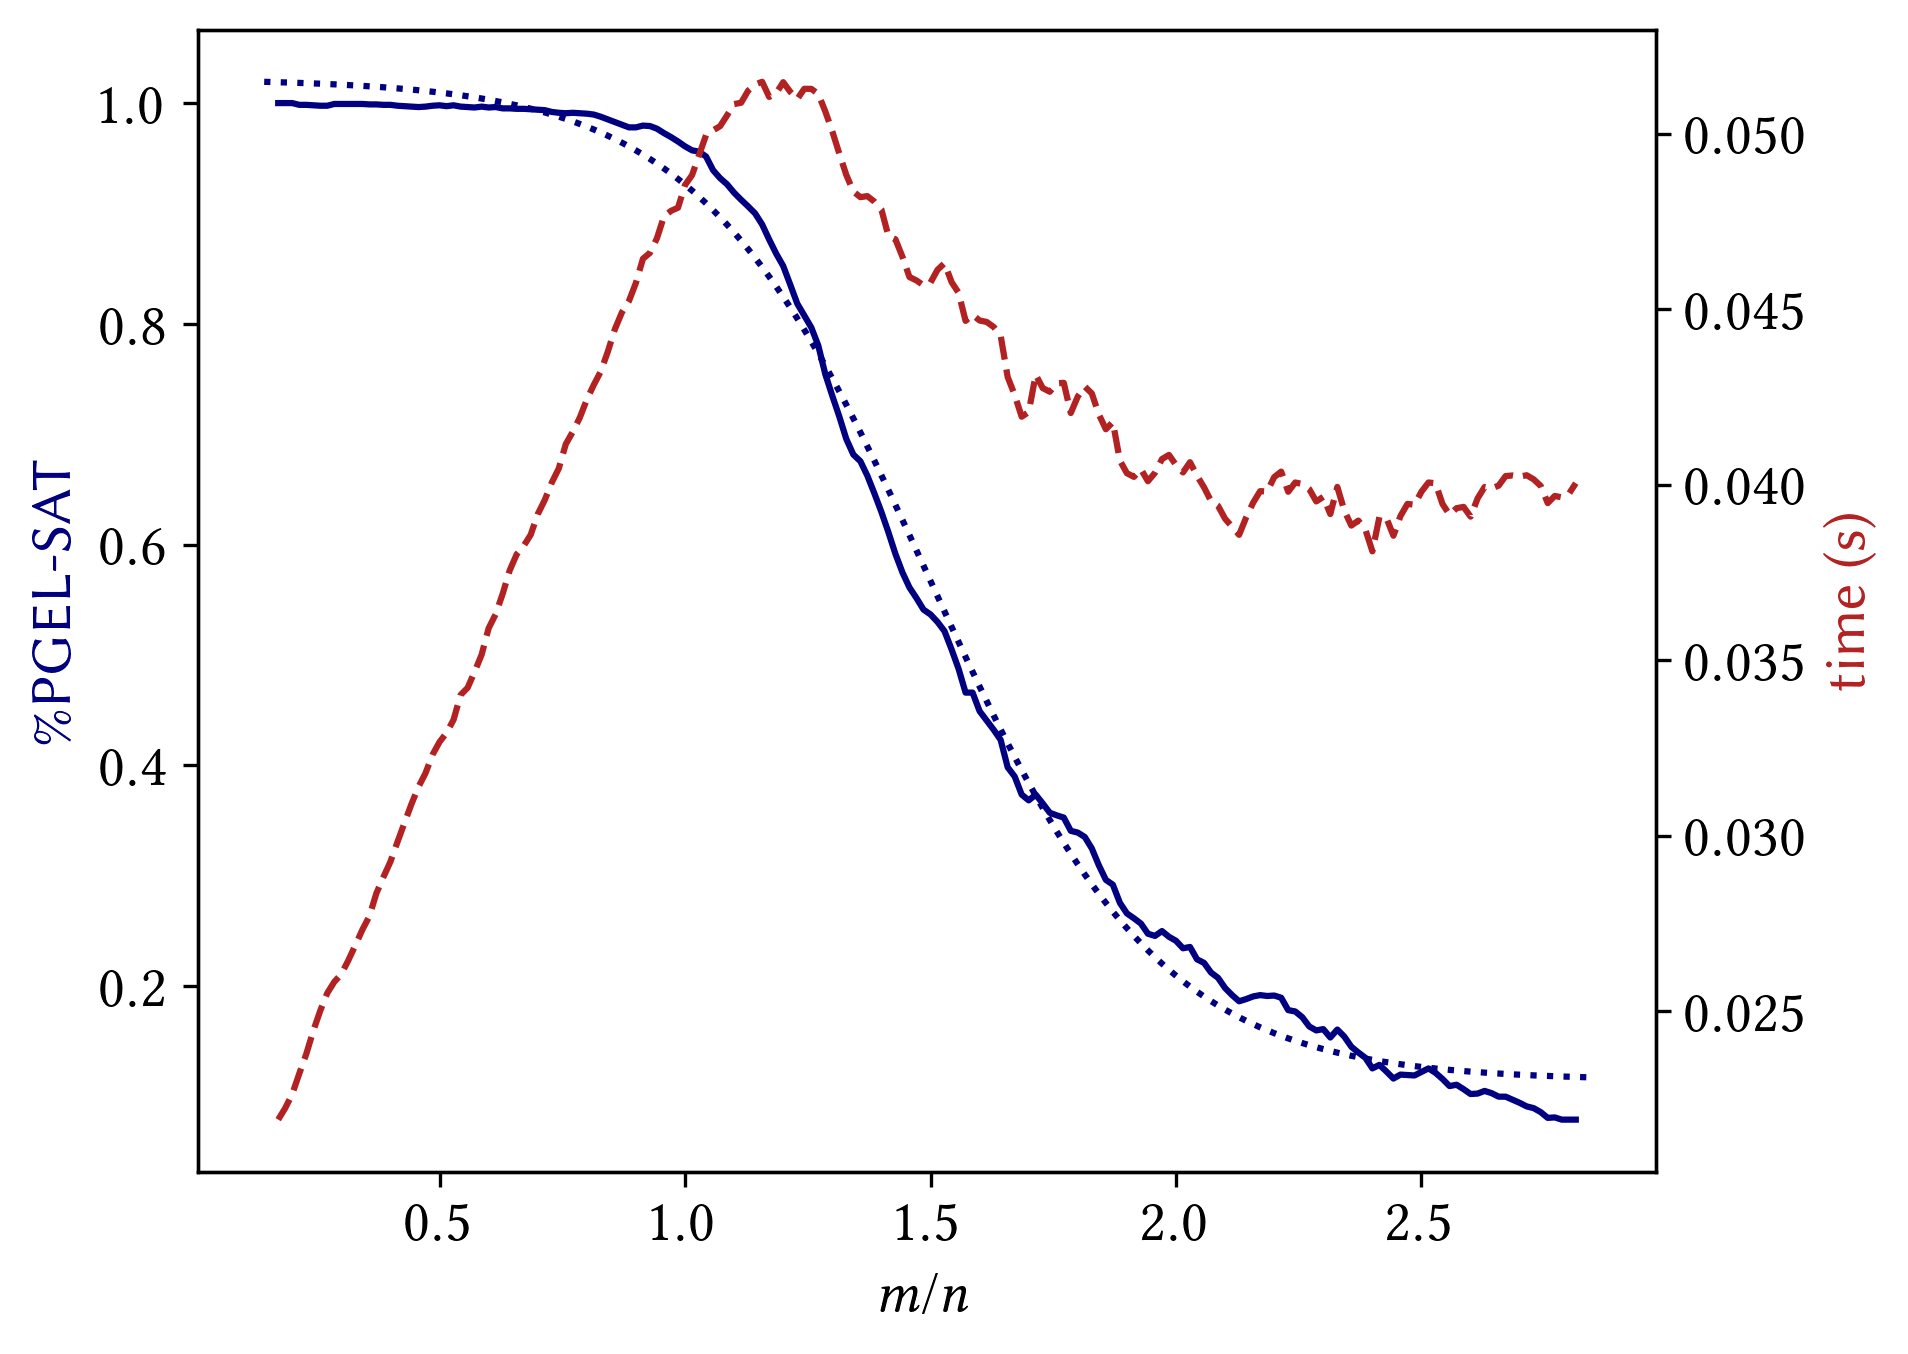
\includegraphics[width=.75\textwidth]{../img/plot-phase-trans}
  \caption{\%-satisfiable of $\pgelsat$ and average run time for instances of formulas in several cases}
  \label{fig:plot-phase}
\end{figure}
  

These experiments show that:
\begin{enumerate}[label=(\alph*)]
	\item There is an S-shaped first-order phase transition, from mostly satisfiable to mostly unsatisfiable, like its propositional problem;
	\item There is not a second-order phase transition. We can see that, when $m/n$ increases, the average time increses until the ratio of satisfiability starts to decrease. This can be explained because the algorithm tries to find an inconsistency. Consequently, when the axioms or restrictions are higher, it is easier to find such inconsistency. \todo{Modify this}
\end{enumerate}

\section{Run time analysis}

This experiment aims to estimate empirically the time complexity of the algorithm and verify its tractability.

Consider a probabilistic KB as defined in \autoref{sec:phase-trans}. Create three experiments for each parameter $n, m$ and $p$; varying one parameter and fixing others. For each value of the varying parameter, generate several instances of $\pgel$-KBs as described in \autoref{sec:phase-trans}.

For this experiment, the fixed parameters had the values $n = 10, n_R = 3, m = 10$ and $p = 10$. Each parameter $n, m$ and $m$ varied from $10$ to $400$ in steps of $20$. For each varying value, we generated $100$ instances of $\pgelsat$, computed the average run time, average run time of a single iteration and number of iterations. Also, it is applied a simple moving average with an window of 5 points to the curves.  Then, we obtained the graphics in \autoref{fig:plot-comp-1}, \autoref{fig:plot-comp-2} and \autoref{fig:plot-comp-3}. 

These experiments show that:
\begin{enumerate}[label=(\alph*)]
  \item The increase of axioms and concepts has low impact in the run time and the number of iterations;
  \item The increase of uncertain axioms has high impact in the run time;
  \item The number of iterations increases linearly with the number of uncertain axioms.
\end{enumerate}
Then, we have a result similar to the estimated complexity in \autoref{sec:time-compl}.

However, one could argue that the run time growth of varying uncertain axioms is exponential. Thus, we propose a new experiment to analyse this curve.

Using the same data from the previous experiment, we applied the Levenberg–Marquardt algorithm \citep{levenberg1944method,marquardt1963algorithm}, which is a method for solving non-linear least squares problems. This method was applied with the SciPy's implemention called \textsf{curve\_fit} \citep{2020SciPy-NMeth}. 

Define a polinomial $p(x)$ and an exponential function $e(x)$, such that
\begin{align*}
  p(x) &:= A_7 \cdot x^7 + A_6 \cdot x^6 + A_5 \cdot x^5 +A_4 \cdot x^4 + A_3 \cdot x^3 + A_2 \cdot x^2 + A_1 \cdot x + A_0\\
  e(x) &:= B_2 \cdot 2^{B_2 \cdot x} + B_0.
\end{align*}
We want to find parameters $A_0, \dots, A_7$ and $B_0, \dots, B_2$ in such a way that $p(x)$ and $e(x)$ best approximate the experimental measures. 

After applying the algorithm, we obtain $p(x)$ and $e(x)$ with the following approximated parameters, which are illustrated in the \autoref{fig:plot-comp-prob},
\begin{align*}
  p(x) :=& -1.5  \cdot  10^{-15} \cdot x^7 
        + 2 \cdot 10^{-12} \cdot x^6 
        - 1 \cdot 10^{-9} \cdot x^5 
        + 2.9 \cdot 10^{-7} \cdot x^4\\ 
        &- 4 \cdot 10^{-5} \cdot x^3 
        + 2.8  \cdot  10^{-3}\cdot x^2 
        - 0.08 \cdot x 
        + 0.64\\
  e(x) :=& \, 0.282 \cdot 2^{0.014 \cdot x} - 0.592.
\end{align*}
From this analysis, we have that:
\begin{enumerate}[label=(\alph*)]
  \item The terms that mostly contribute to the growth of $p(x)$ have a small degree ($x^4$ and $x^2$);
  \item The factor multipling $x$ in $e(x)$ is small ($\approx 0.014$); therefore, $e(x)$ corresponds to the function $f(x) = 0.282 \cdot (1.01)^{x} - 0.592$, which has a very small exponential growth rate.
\end{enumerate}
Thus, there is no experimental results to refute that the run time growth of \textsc{PGEL-SAT-Solver} is not polynomial. 

\begin{figure}[ht]
  \centering
  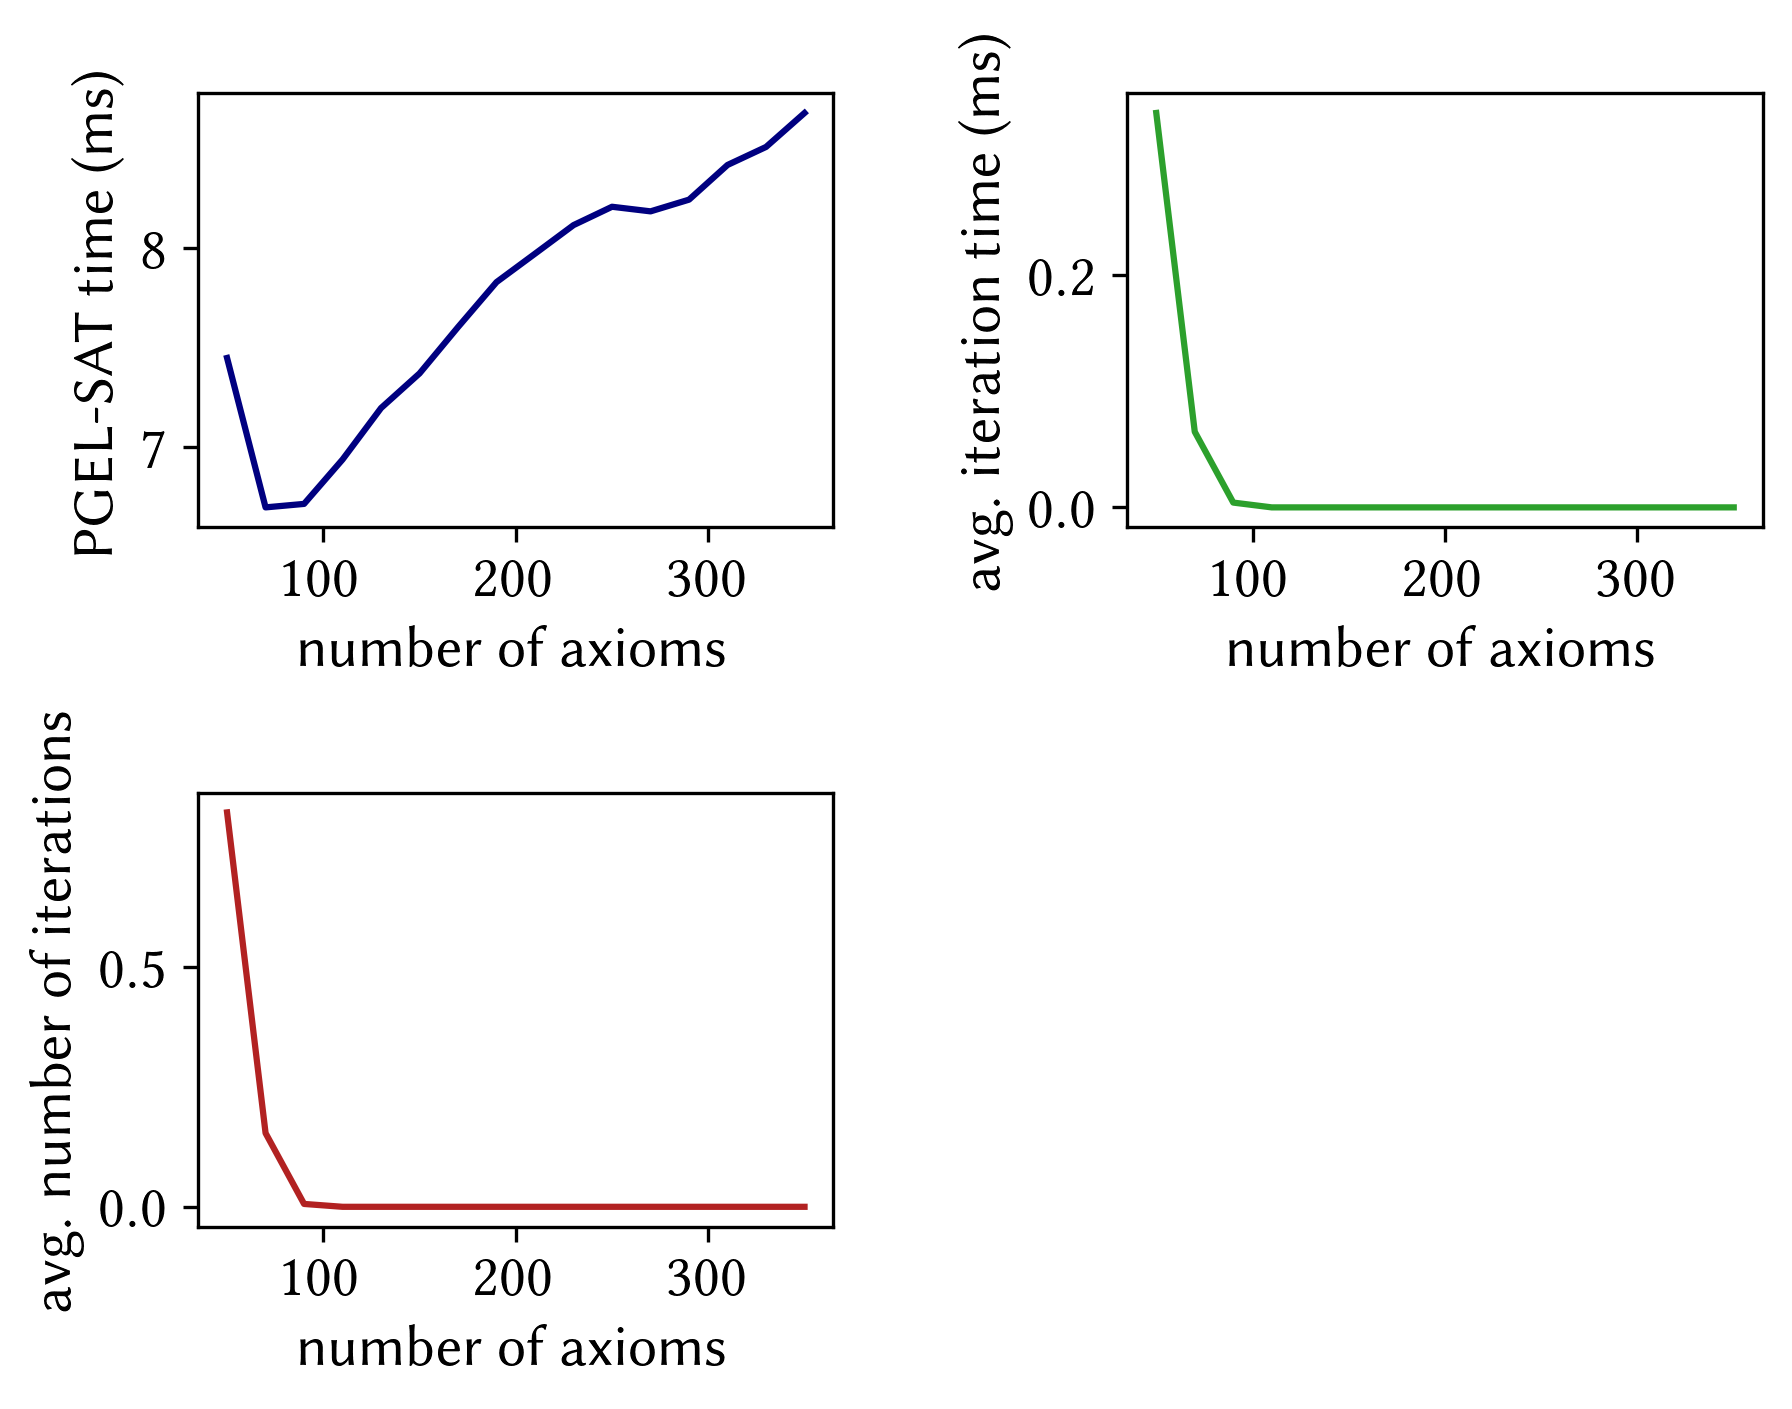
\includegraphics[width=.75\textwidth]{../img/plot-comp1-0}
  \caption{Impact of the increase of certain axioms in the run time and number of iterations}
  \label{fig:plot-comp-1}
\end{figure}

\begin{figure}[ht]
  \centering
  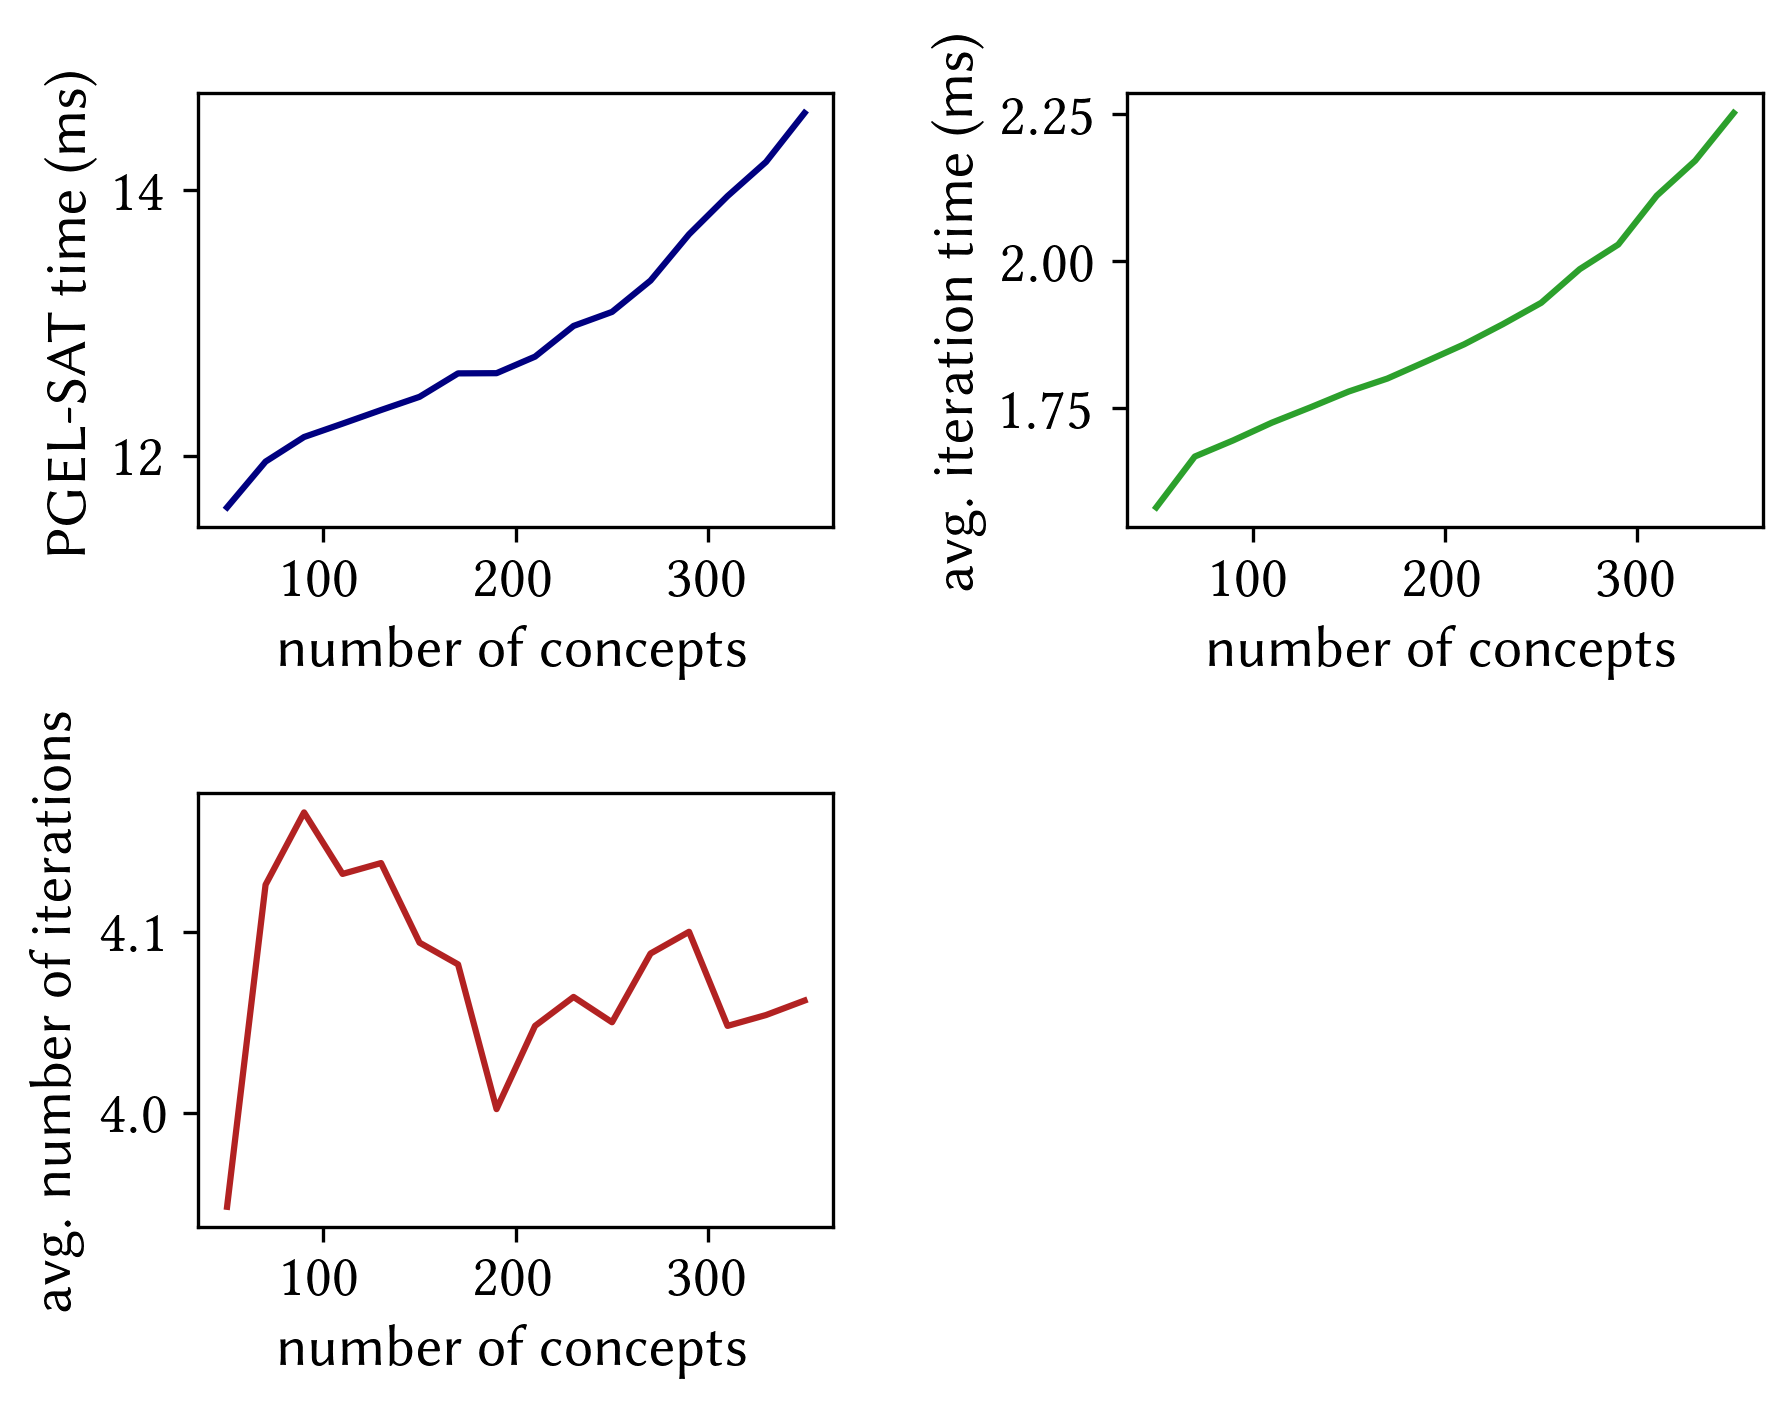
\includegraphics[width=.75\textwidth]{../img/plot-comp1-1}
  \caption{Impact of the increase of concepts in the run time and number of iterations}
  \label{fig:plot-comp-2}
\end{figure}

\begin{figure}[ht]
  \centering
  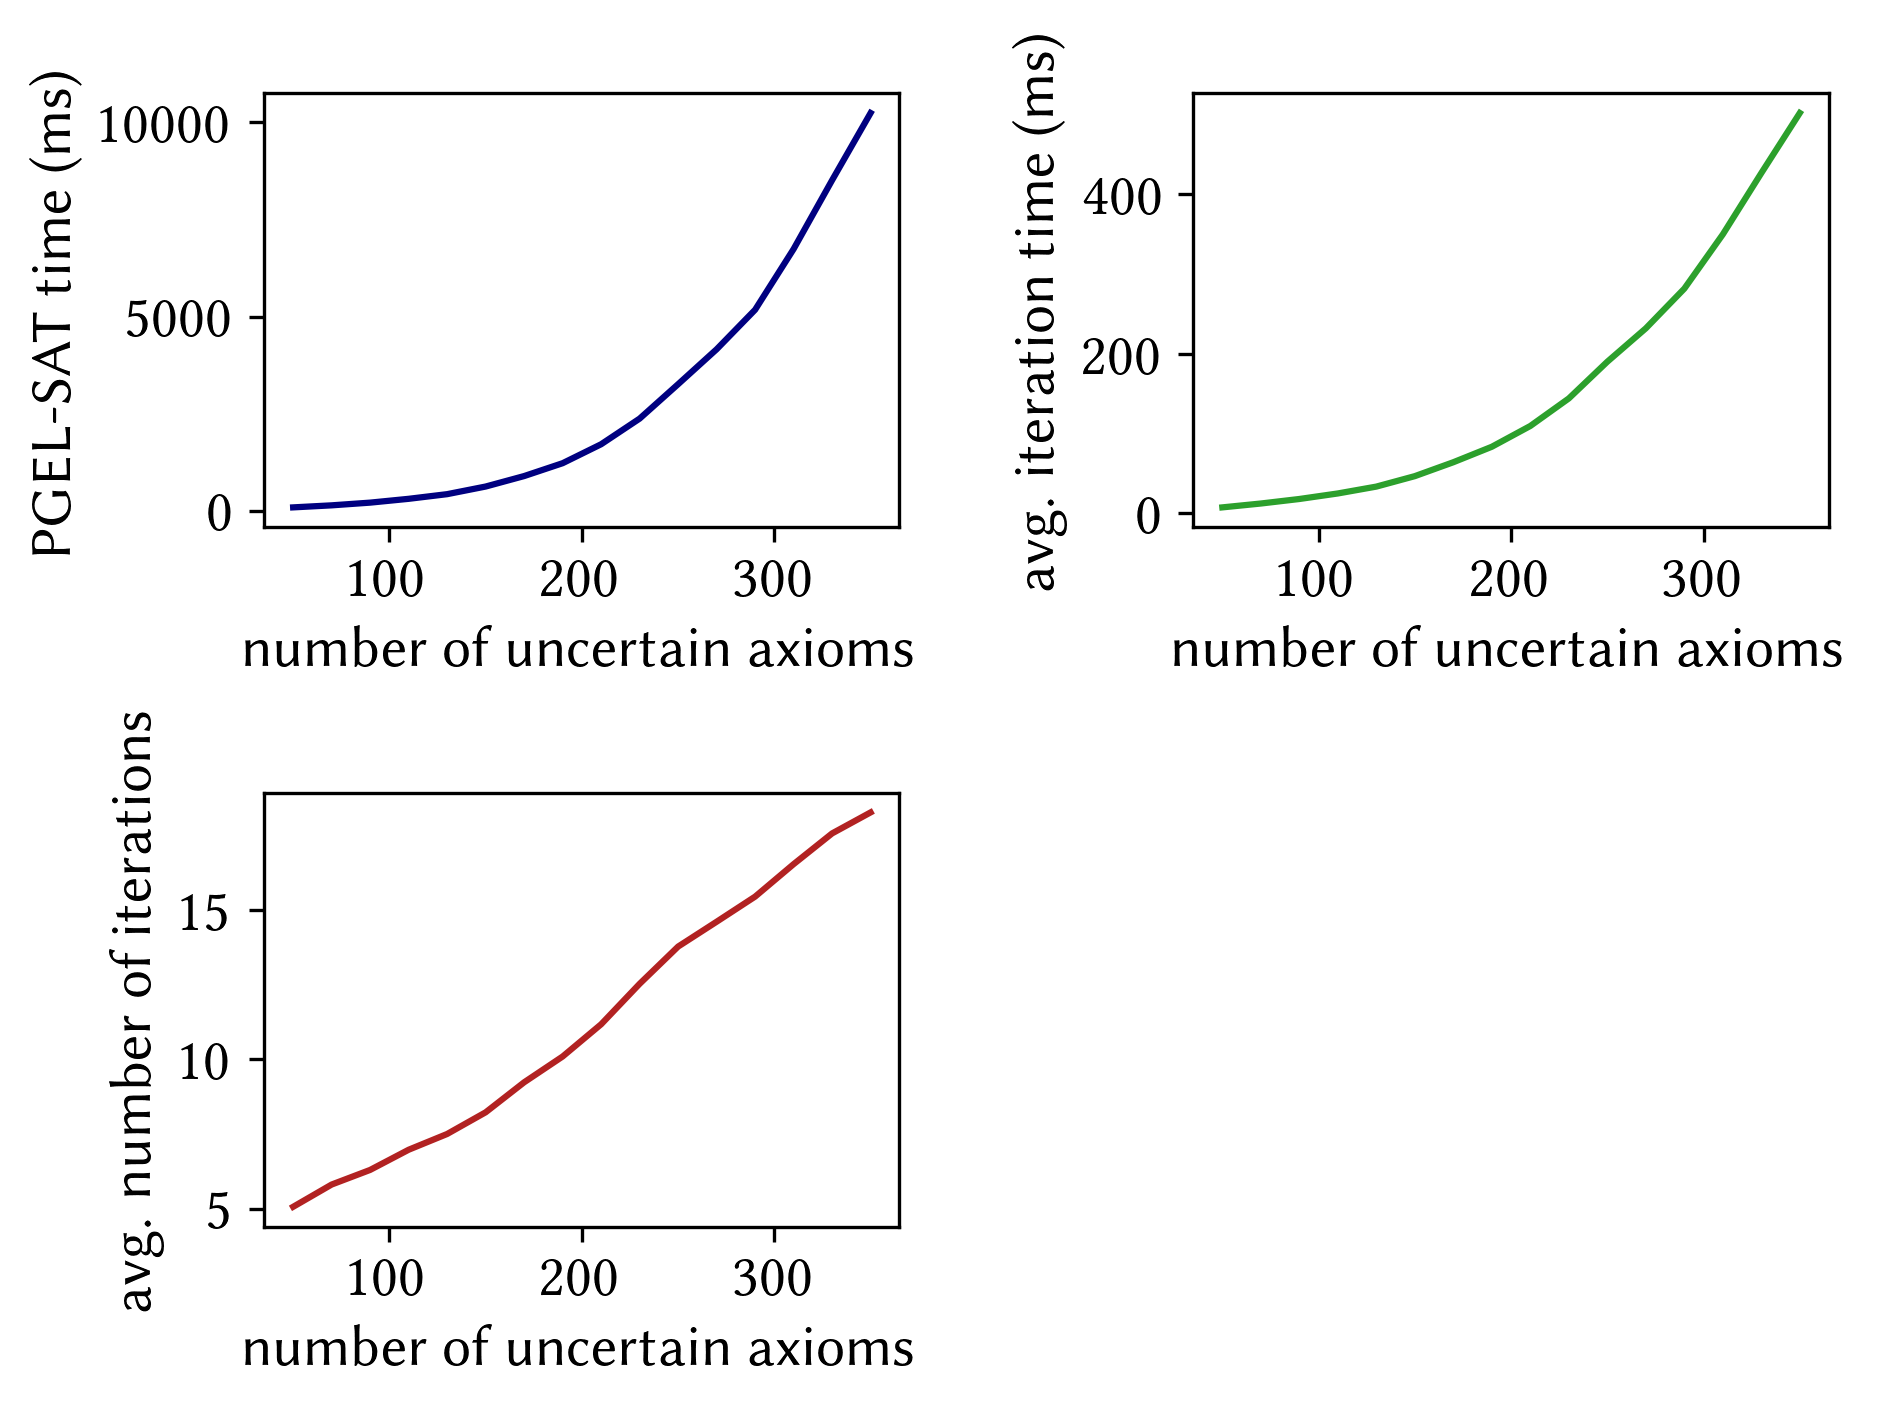
\includegraphics[width=.75\textwidth]{../img/plot-comp1-2}
  \caption{Impact of the increase of uncertain axioms in the run time and number of iterations}
  \label{fig:plot-comp-3}
\end{figure}

\begin{figure}[ht]
  \centering
  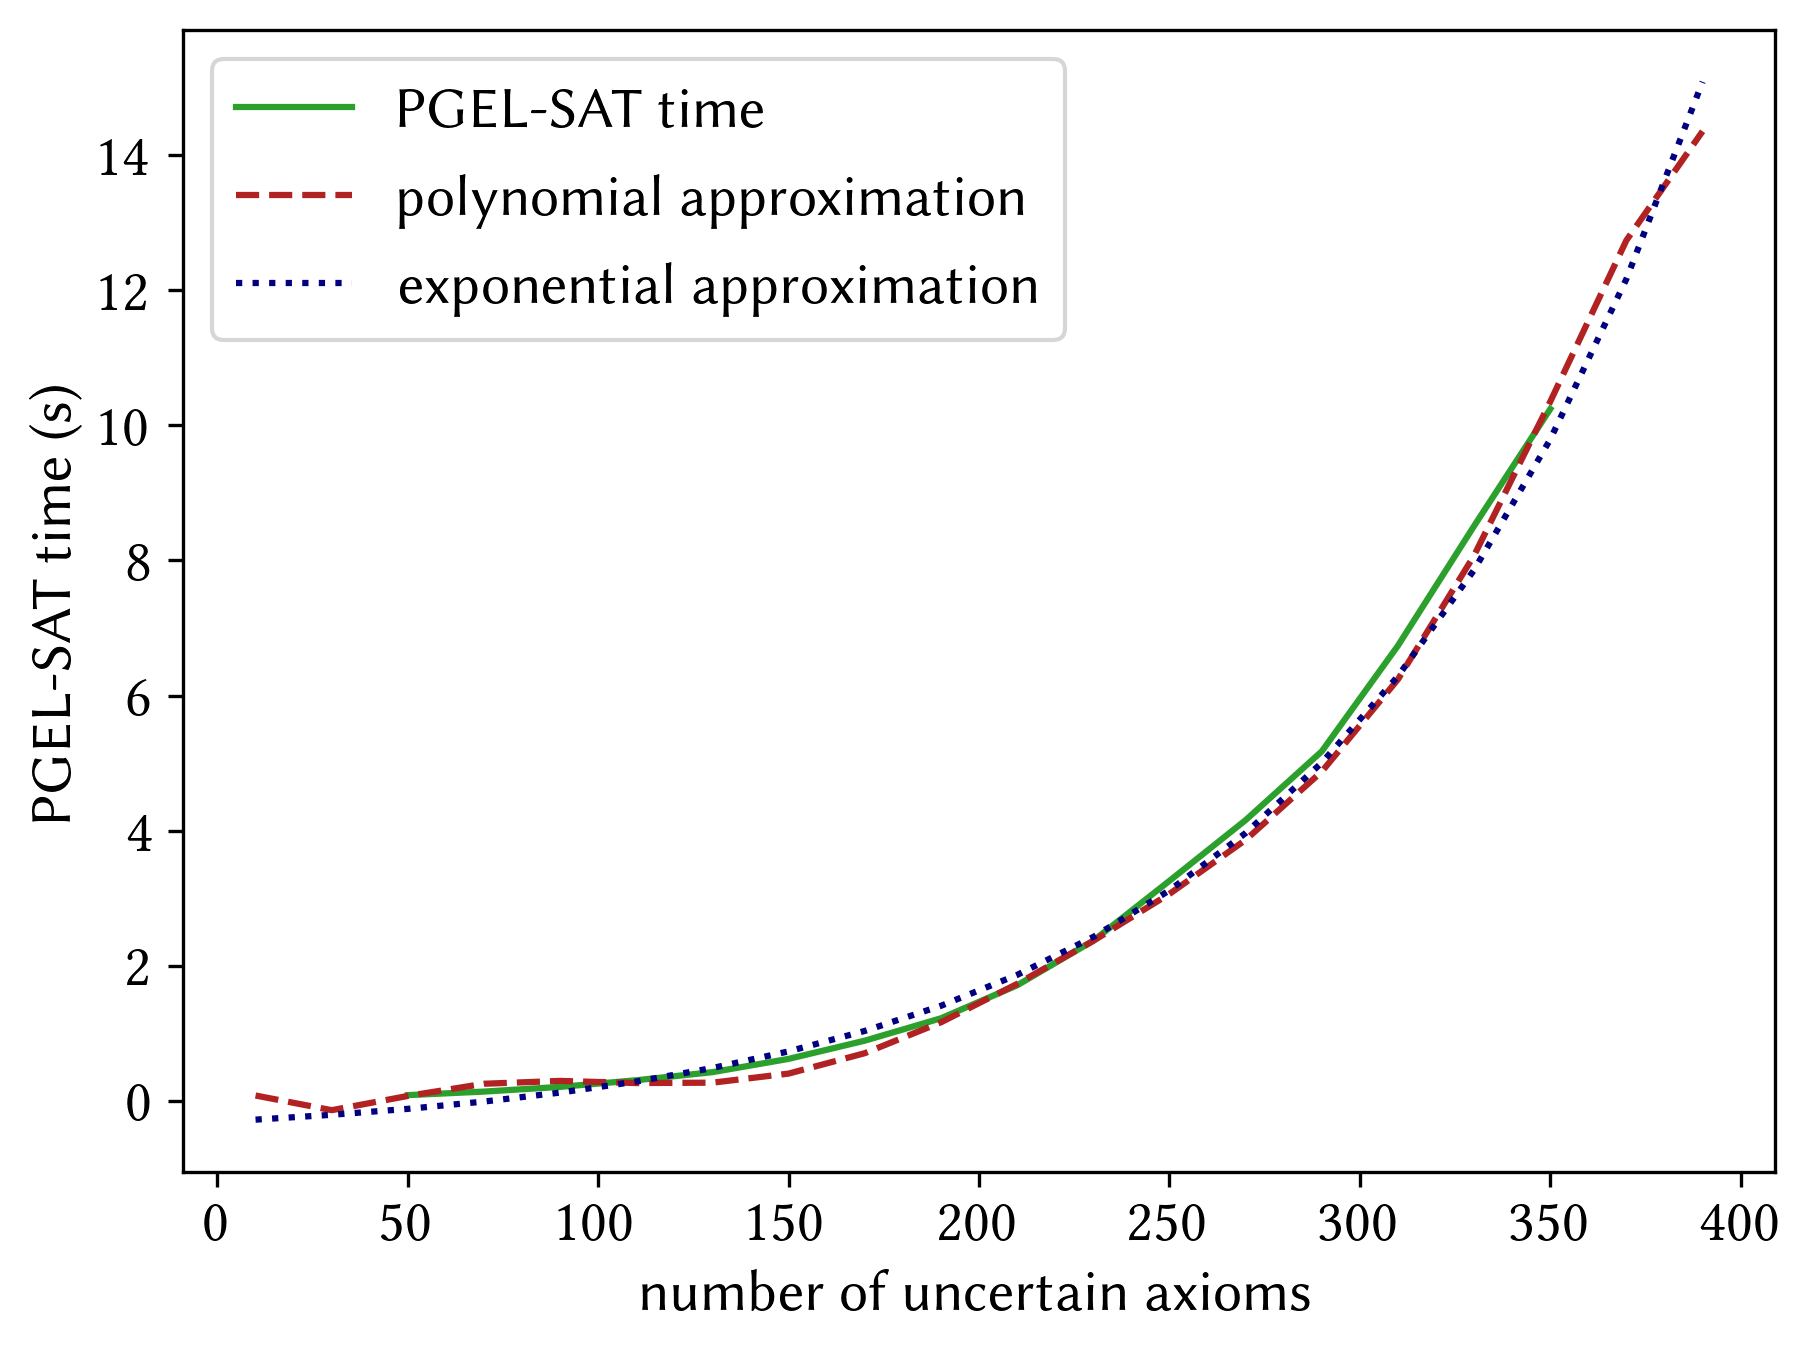
\includegraphics[width=.75\textwidth]{../img/plot-comp2}
  \caption{Polynomial and exponential approximations of the run time growth by varying the number of uncertain axioms}
  \label{fig:plot-comp-prob}
\end{figure}

As expected, these algorithms do not have the phase transition behavior of NP-Complete problems and do not show any exponential run time growth rate. Then, these initial experiments confirm that \textsc{PGEL-SAT-Solver} is a promising algorithm for tractable probabilistic reasoning over description logics.

  %!TeX root=../tese.tex

\chapter{Related work}
\label{cap:relatedwork}

The problem of probabilistic reasoning and extensions in logics to deal with uncertainty have been studied for several decades. The first known proposal of PSAT, for propositional formulas, is attributed to \citet{boole1854investigation} and it has already been shown to be NP-Complete \citep{georgakopoulos1988probabilistic}.

In the relational domain, the literature contain several logics with probabilistic reasoning capabilities although they have led to intractable decision problems.  Some of them extend the already intractable $\mathcal{ALC}$, with probabilistic constrains over concepts \citep{heinsohn1994probabilistic, lukasiewicz2008expressive, GutierrezBasultoEA11}. For the expressive and lightweight $\el$-family, some extensions such as \citet{gutierrez2017probabilistic,ceylan2017bayesian} have led to \textsc{ExpTime}-hard or PP-complete probabilistic reasoning; futhermore, NP-completeness can be achieved with probability capabilities over axioms \citep{Fin2019b}.

On the other hand, many results implies that the research on Max-SAT has a impact on the solutions of PSAT problems \citep{andersen2001easy}. Also, there was already proposed a MaxSAT-solver for a propositional fragment of horn logic by a max-flow/min-cut formulation \citep{jaumard1987complexity}. Thus, it is expected to ask if one could also take such results to a relational domain.

  %!TeX root=../tese.tex

\chapter{Conclusion and future work}
\label{cap:conclusion}

Different studies focused on description logics with probabilistic reasoning. In particular, finding a logic that is both tractable and expressive enough became a problem of special interest in the field.

- this work proposed a fragment of el++ with probabilistic capabilities.

- probabilistic description logics are important

- proposed solution is polynomial

- an upper bound of O() was estimated and experimental analysis confirm the polynomial complexity of the run time. 

- future work

- modeling of existential body axioms and conjunctive axioms using probabilistic restrictions

- modeling of conditional probabilities

\todo[inline]{add conclusion}

  \par

  %%%%%%%%%%%%%%%%%%%%%%%%%%%% APÊNDICES E ANEXOS %%%%%%%%%%%%%%%%%%%%%%%%%%%%%%%%

  % Um apêndice é algum conteúdo adicional de sua autoria que colabora com a
  % ideia geral do texto mas que, por alguma razão, não precisa fazer parte
  % da sequência do discurso; por exemplo, a demonstração de um teorema, as
  % perguntas usadas em uma pesquisa qualitativa etc.
  %
  % Um anexo é um documento que não é de sua autoria mas que é relevante para
  % a tese; por exemplo, a especificação do padrão que o trabalho discute.
  %
  % Os comandos appendix e annex reiniciam a numeração de capítulos e passam
  % a numerá-los com letras. "annex" não faz parte de nenhuma classe padrão,
  % ele foi criado para este modelo (em annex.sty e utils.tex). Se o
  % trabalho não tiver apêndices ou anexos, remova estas linhas.
  %
  % Diferentemente de \mainmatter, \backmatter etc., \appendix e \annex não
  % forçam o início de uma nova página. Em geral isso não é importante, pois
  % o comando seguinte costuma ser "\chapter", mas pode causar problemas com
  % a formatação dos cabeçalhos. Assim, vamos forçar uma nova página antes
  % de cada um deles.

  %%%% Apêndices %%%%
  % \makeatletter
  % \if@openright\cleardoublepage\else\clearpage\fi
  % \makeatother

  % Este formato está definido na package imeusp-headers.
  % \pagestyle{appendix}

  % \appendix

  %\input{conteudo-exemplo/apendices}
  % %!TeX root=../tese.tex

% \input{front-back-matter/appendix/owl-example.tex}
  % \par


  %%%%%%%%%%%%%%%%%%%%%%%%%%%%%% SEÇÕES FINAIS %%%%%%%%%%%%%%%%%%%%%%%%%%%%%%%%%%%

  % Aqui vão a bibliografia, índice remissivo e outras seções similares.

  % O comando backmatter desabilita a numeração de capítulos.
  \backmatter

  % Este formato está definido na package imeusp-headers
  \pagestyle{backmatter}

  % Espaço adicional no sumário antes das referências / índice remissivo
  \addtocontents{toc}{\vspace{2\baselineskip plus .5\baselineskip minus .5\baselineskip}}

  % A bibliografia é obrigatória
  %%%%%%%% Bibliografia com biblatex (preferido): %%%%%%%%

  \printbibliography[
    title=\refname\label{bibliography}, % "Referências", recomendado pela ABNT
    heading=bibintoc,
  ]

  % imprime o índice remissivo no documento (opcional)
  % \printindex

\end{document}
